\documentclass{beamer}
\usetheme{Madrid}
\usepackage{booktabs}
\usepackage{listings}
\usepackage{tikz}
\usepackage{amsmath}

%Information to be included in the title page:
\title{Prouver l'exécution d'un automate (STARK)}
\author{Mathéo Le Dévéhat}
\institute{23112}
\date{2025-2026}

\begin{document}
\frame{\titlepage}

\begin{frame}
\frametitle{Sommaire}
\tableofcontents
\end{frame}
\AtBeginSection[]
{
  \begin{frame}
    \frametitle{Sommaire}
    \tableofcontents[currentsection]
  \end{frame}
}
\section{Objectif et motivations}
\begin{frame}
\frametitle{Objectif}
Sachant un automate A, prouver qu'on connaît un mot w tel que l'automate reconnaisse ce mot sans le divulguer.

\begin{figure}[h!]
  \centering
  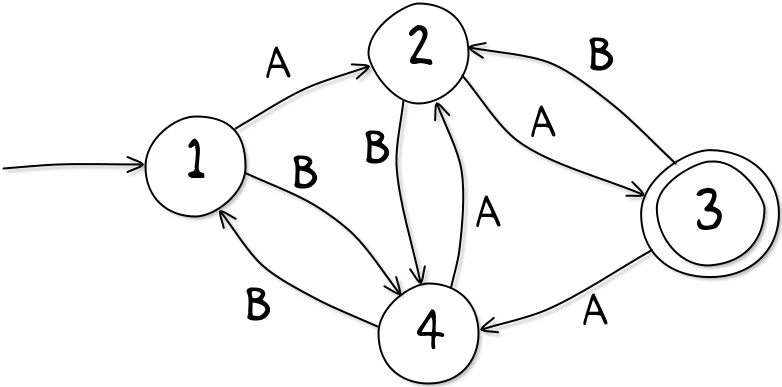
\includegraphics[width=0.8\textwidth]{automata.png}
  \caption{Un exemple d'automate (csfieldguide.org.nz)}
\end{figure}

\end{frame}

\begin{frame}
\frametitle{Motivations}
Permet de prouver son identité sans révéler des informations supplémentaires.
\end{frame}
\AtBeginSection[]
{
  \begin{frame}
    \frametitle{Sommaire}
    \tableofcontents[currentsection]
  \end{frame}
}
\section{Prérequis}

\begin{frame}
\frametitle{Prérequis: Fonction de hachage}

\begin{figure}[h!]
  \centering
  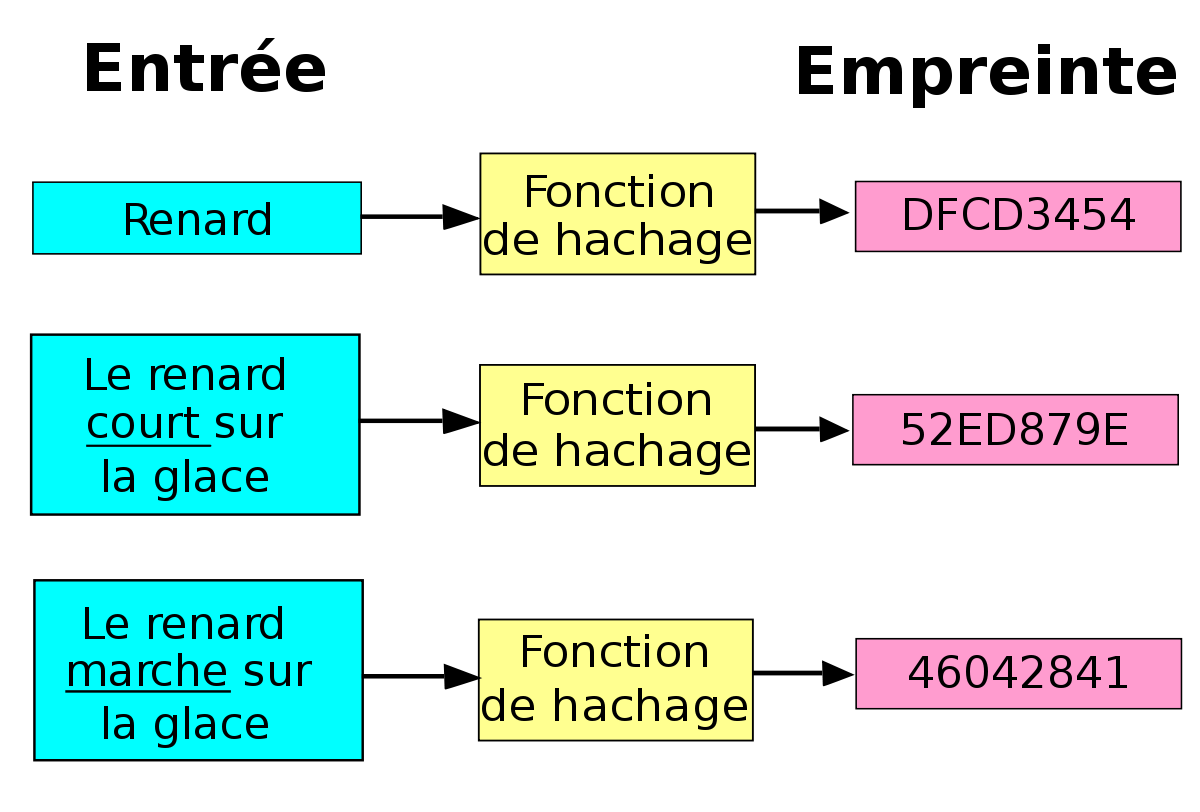
\includegraphics[width=0.5\textwidth]{hash.png}
  \caption{Illustration d'une fonction de hachage (techno-science.net)}
\end{figure}

Critères essentiels:
\begin{enumerate}
	\item Résistance aux collisions
	\item Résistance à la préimage
	\item  Résistance à la deuxième préimage
	\item Distribution uniforme
\end{enumerate}

\end{frame}

\begin{frame}
\frametitle{Prérequis: Arbres de Merkle}

\begin{figure}[h!]
  \centering
  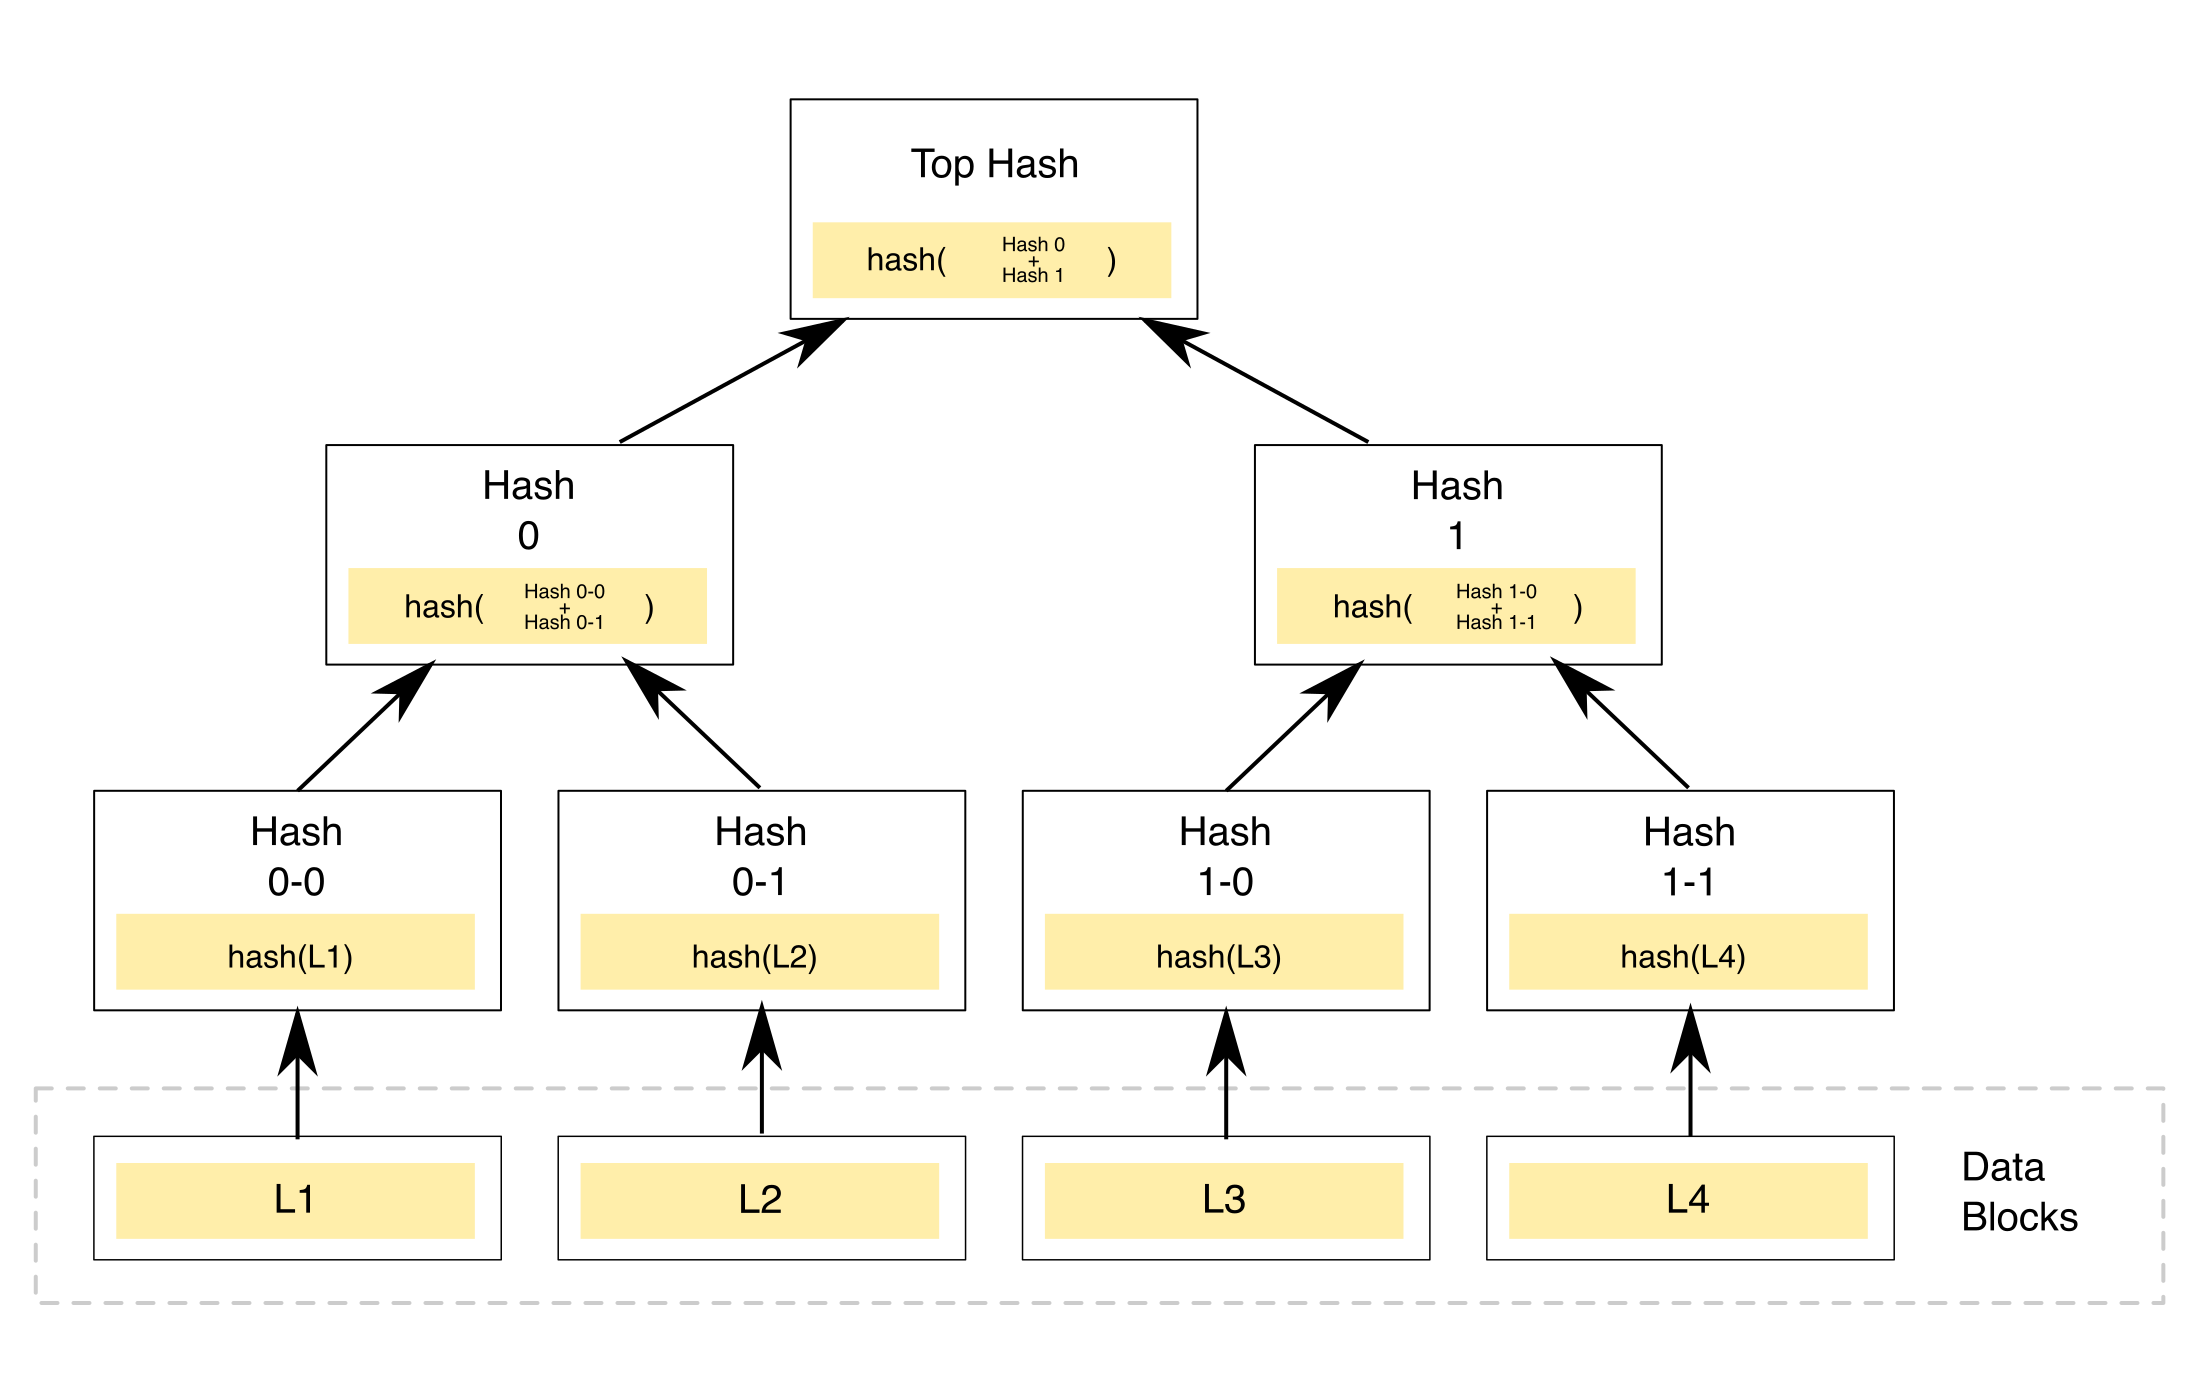
\includegraphics[width=0.8\textwidth]{merkle.png}
  \caption{Un exemple d'arbre de Merkle (wikipedia.org)}
\end{figure}

\end{frame}

\begin{frame}{Attestation d'une valeur spécifique}
    \begin{columns}[T]

        % Colonne de gauche : Explications et Formule
        \begin{column}{0.5\textwidth}
            % \vspace{0.3cm}
            \textbf{Le Chemin d'Authentification}
            % \vspace{0.2cm}
            \begin{itemize}
                \item Pour prouver qu'une feuille (\textcolor{green!60!black}{\textbf{Valeur $L_3$}}) appartient à l'arbre, on ne transmet pas tout l'arbre.
                \item On fournit uniquement les \textbf{nœuds frères} sur le chemin (\textcolor{orange}{\textbf{nœuds oranges}}).
                \item Le vérificateur recalcule les parents itérativement (\textcolor{blue}{\textbf{nœuds bleus}}) jusqu'à la racine.
            \end{itemize}

            % \vspace{0.5cm}

            % \vspace{0.3cm}
            \small{\textit{Efficacité :} La taille de la preuve n'est que de $\mathcal{O}(\log_2(N))$ éléments, rendant les STARKs très compacts pour de grandes traces d'exécution.}
        \end{column}

        % Colonne de droite : Arbre avec TikZ
        \begin{column}{0.5\textwidth}
            \begin{center}
                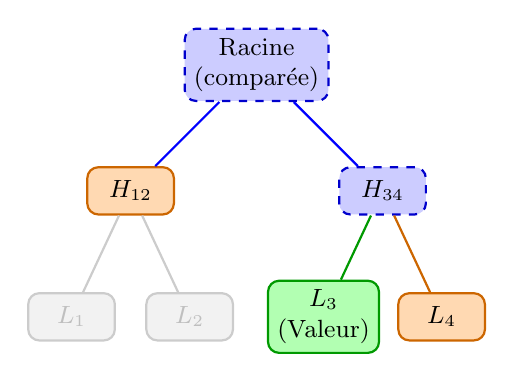
\begin{tikzpicture}[
                    level distance=1.6cm,
                    level 1/.style={sibling distance=3.2cm},
                    level 2/.style={sibling distance=1.5cm},
                    every node/.style={draw, rectangle, rounded corners, align=center, font=\small, minimum width=1.1cm, minimum height=0.6cm},
                    target/.style={fill=green!30, thick, draw=green!60!black},
                    proof/.style={fill=orange!30, thick, draw=orange!80!black},
                    recalc/.style={fill=blue!20, dashed, thick, draw=blue!80!black},
                    normal/.style={fill=gray!10, draw=gray!40, text=gray!50}
                ]

                % Construction de l'arbre
                \node[recalc] (root) {Racine\\(comparée)}
                    child {node[proof] {$H_{12}$}
                        child {node[normal] {$L_1$} edge from parent[draw=gray!40]}
                        child {node[normal] {$L_2$} edge from parent[draw=gray!40]}
                        edge from parent[draw=blue, thick]
                    }
                    child {node[recalc] {$H_{34}$}
                        child {node[target] {$L_3$\\(Valeur)} edge from parent[draw=green!60!black, thick]}
                        child {node[proof] {$L_4$} edge from parent[draw=orange!80!black, thick]}
                        edge from parent[draw=blue, thick]
                    };

                \end{tikzpicture}
            \end{center}
            \begin{block}{Formule de reconstruction}
                \centering
                \vspace{0.2cm}
                $H_{\text{parent}} = \text{Hash}\left(H_{\text{gauche}} \parallel H_{\text{droite}}\right)$
                \vspace{0.2cm}
            \end{block}
        \end{column}

    \end{columns}
\end{frame}

\begin{frame}
\frametitle{Prérequis: L'heuristique de Fiat-Shamir}

\begin{columns}[T]
\begin{column}{0.5\textwidth}
\begin{figure}[h!]
  \centering
  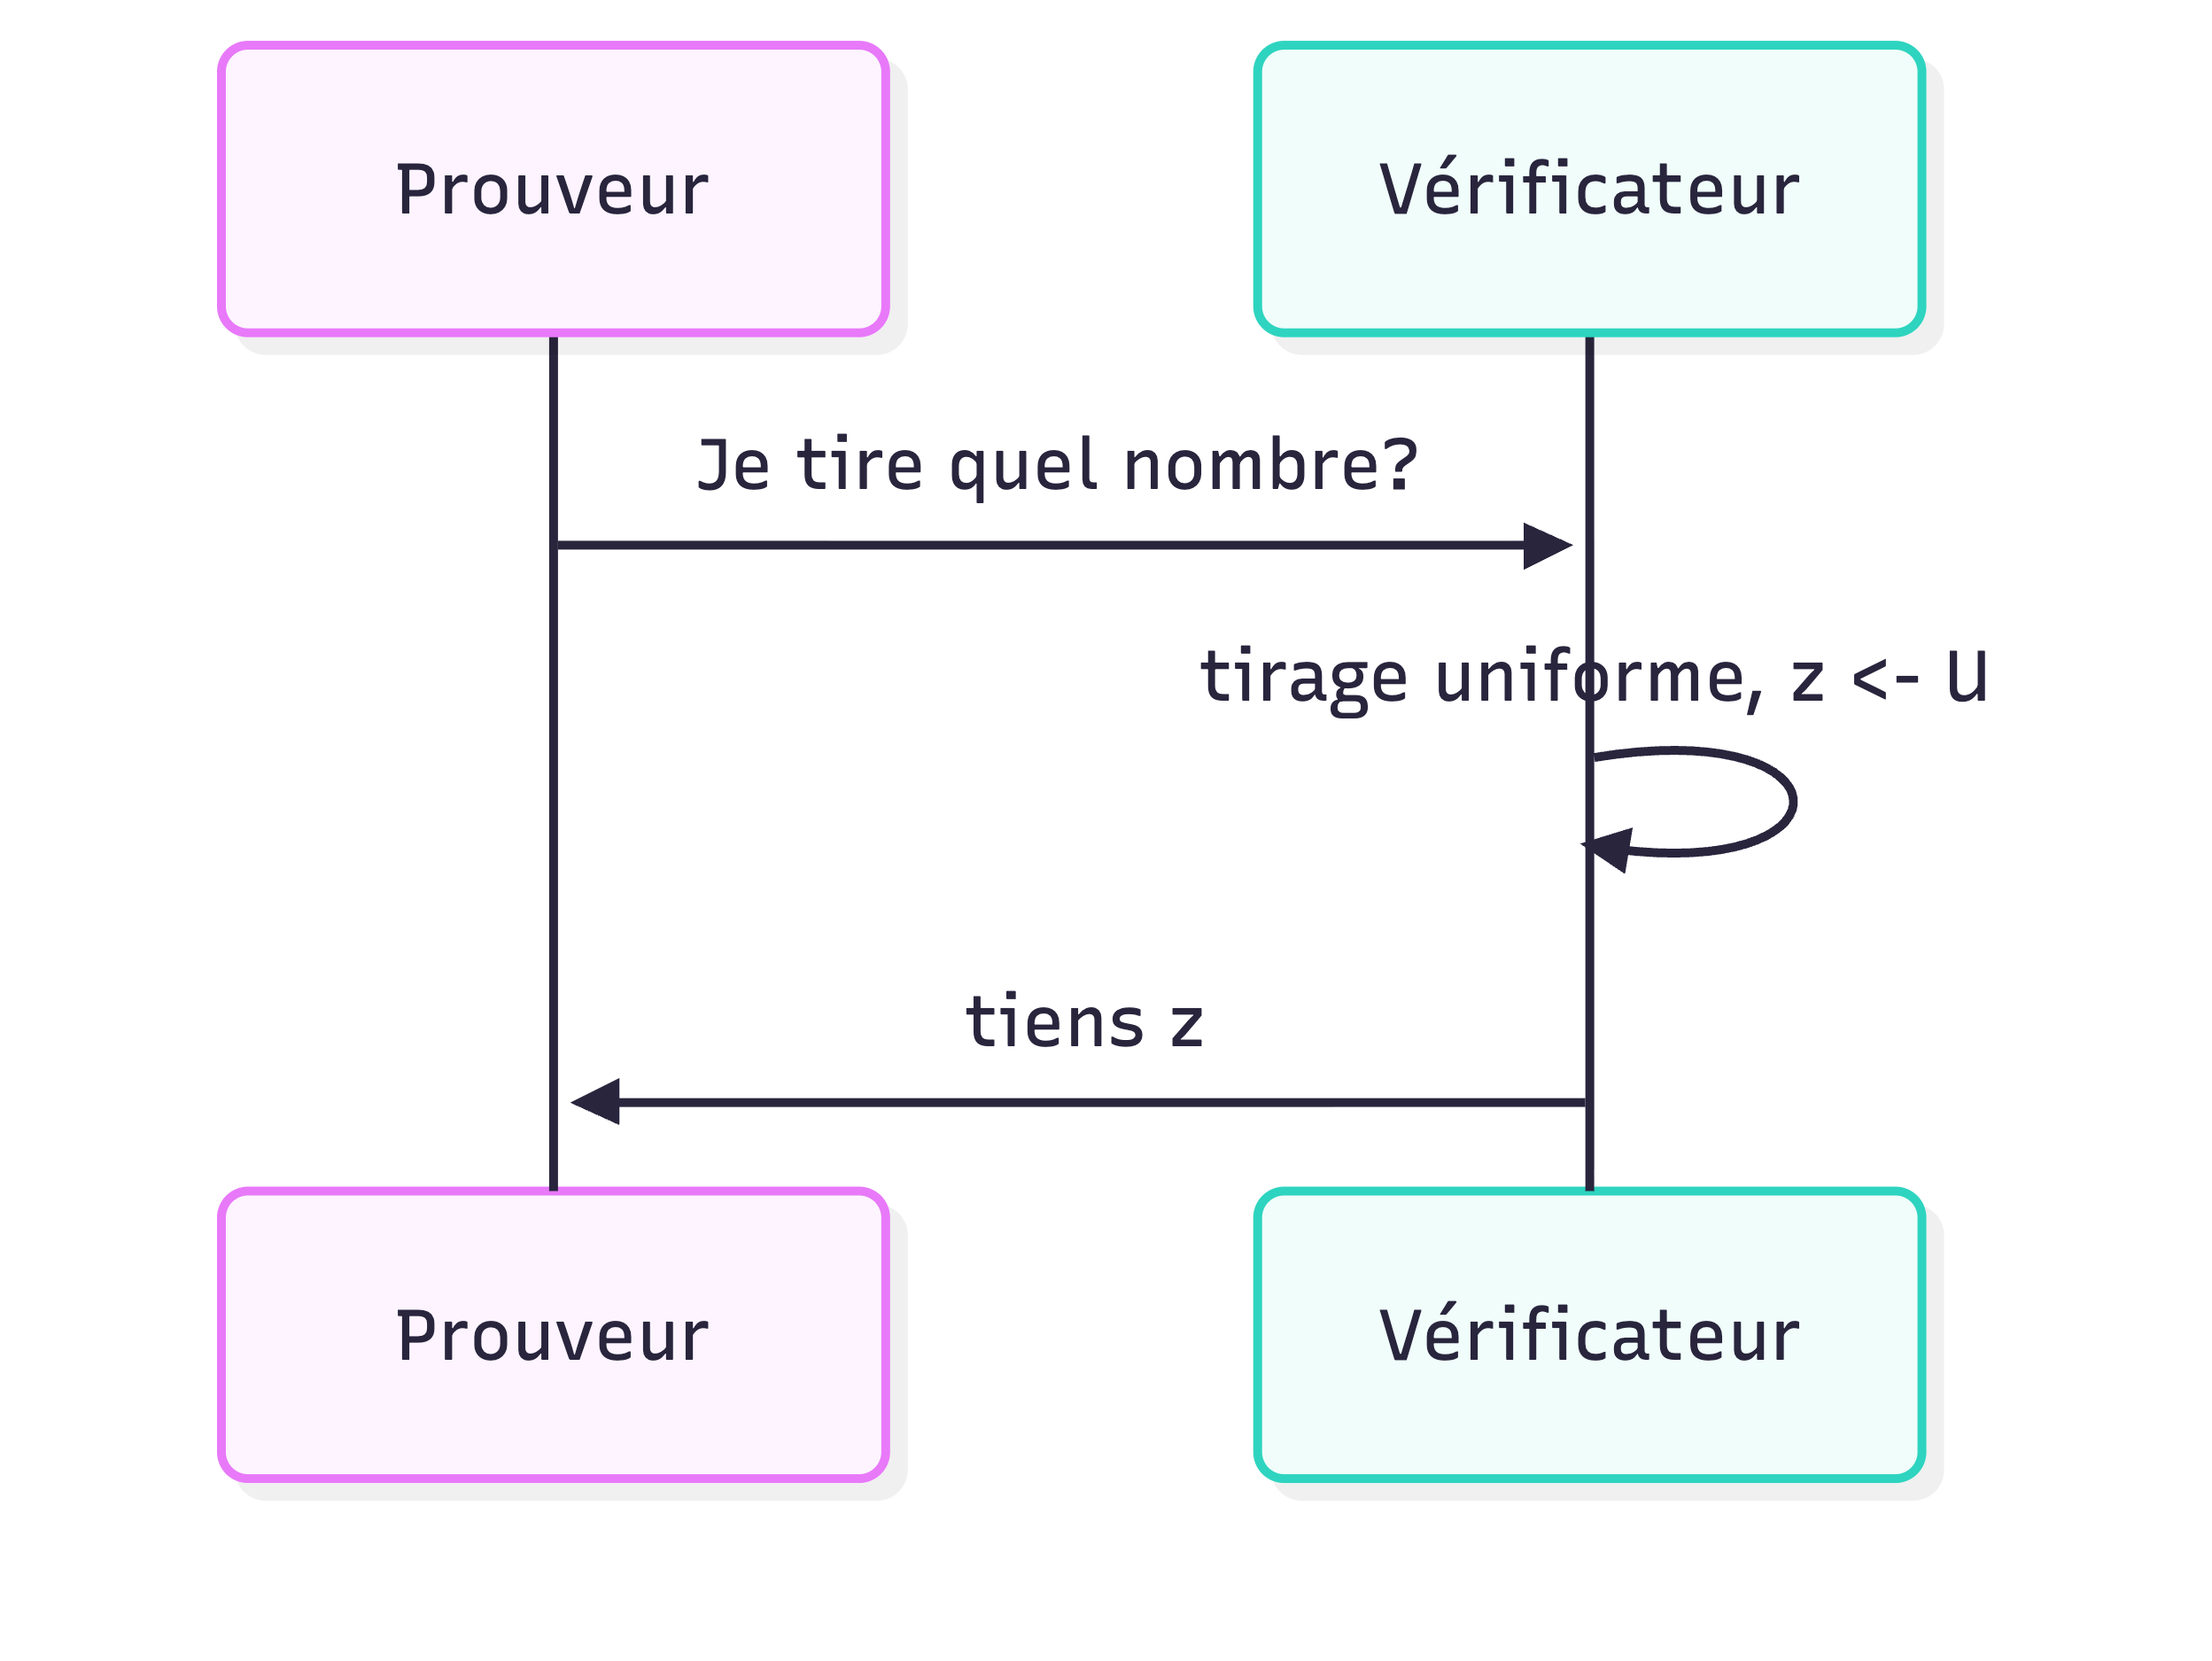
\includegraphics[width=0.8\textwidth]{random-sequence.png}
  \caption{Version intéractive}
\end{figure}
\end{column}
\begin{column}{0.5\textwidth}
\begin{figure}[h!]
  \centering
  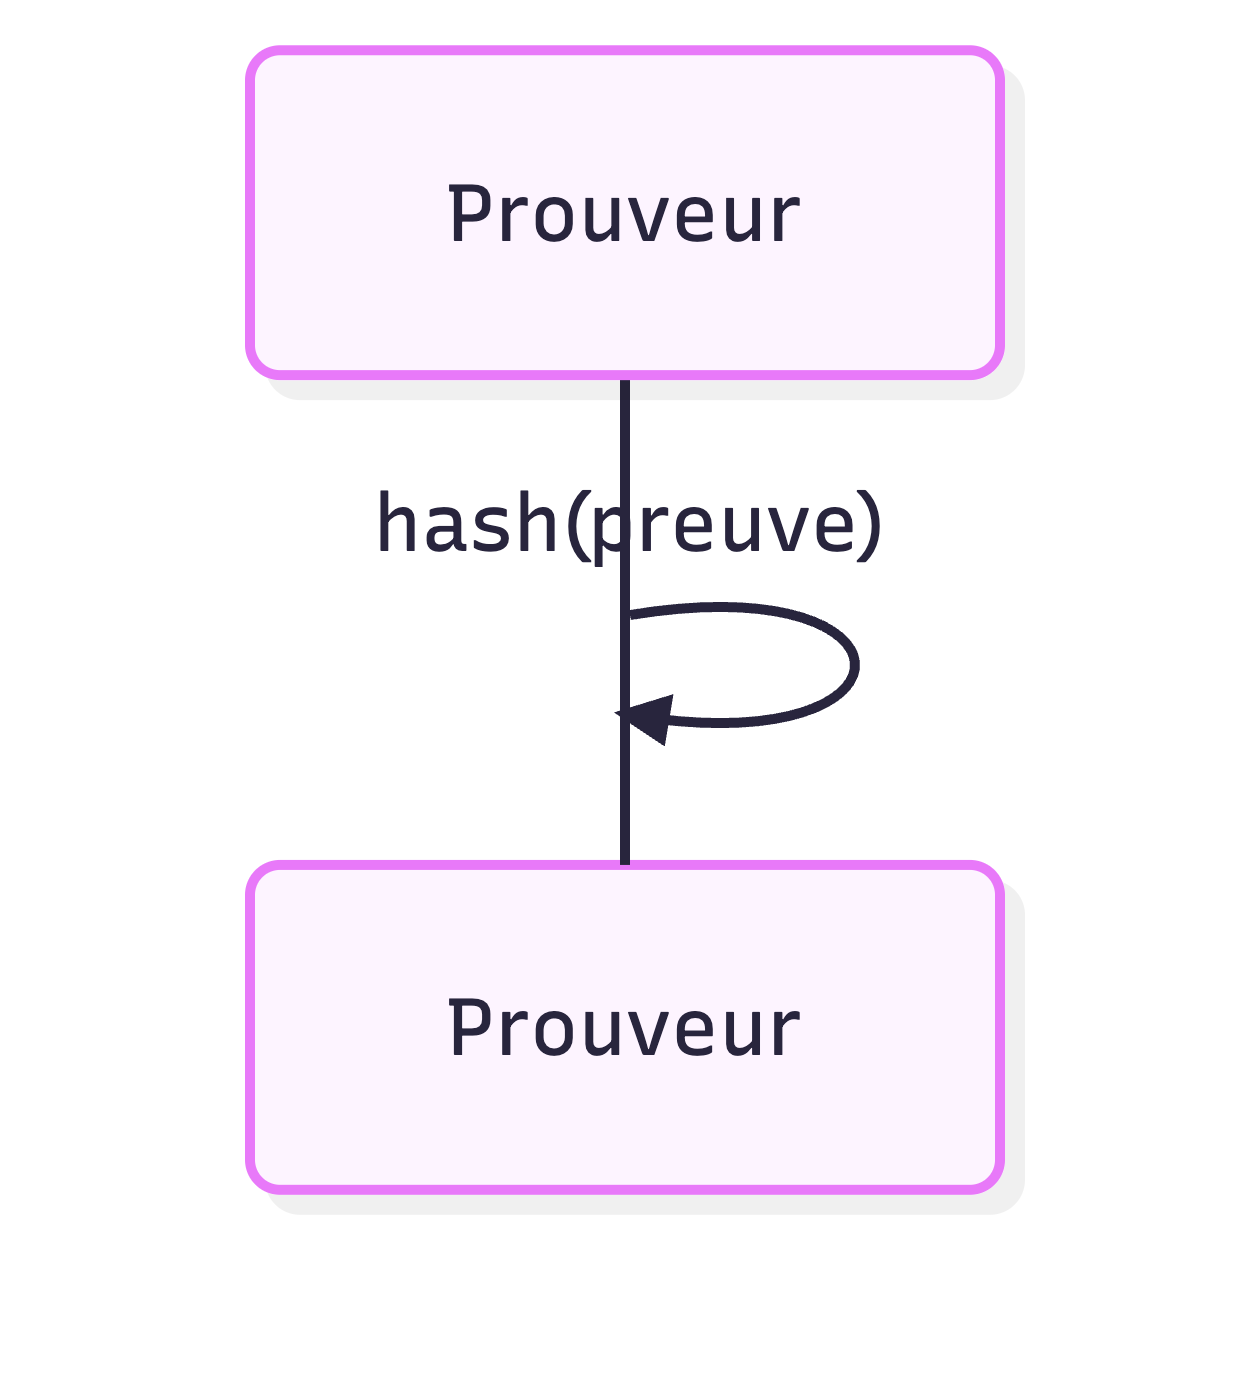
\includegraphics[width=0.8\textwidth]{fiat-shamir.png}
  \caption{Version non intéractive}
\end{figure}
\end{column}
\end{columns}

\end{frame}
\AtBeginSection[]
{
  \begin{frame}
    \frametitle{Sommaire}
    \tableofcontents[currentsection]
  \end{frame}
}
\section{Définitions}

\begin{frame}
\frametitle{Architecture ZK-STARK}

\begin{block}{Définition ZK-STARK}
Zero-Knowledge, Succint, Transparent, Argument of Knowledge. En français, argument succint et transparent de connaissance à divulgation nulle de connaissance, ie. prouver qu'on connaît un certain $w$ (témoin) satisfiant une propriété $P$ sans divulguer $w$.
\end{block}

\begin{flushleft}
Une Architecture de ZK-STARK se compose de deux entités, le prouveur et le vérificateur. Généralement le prouver est une entité centrale qui a une grosse puissance de calcul et des données qu'elle souhaite garder privées et le vérificateur est accessible publiquement et à une puissance de calcul moindre. Cas d'usage: vérification de programmes lourds sur une blockchain publique.
\end{flushleft}

\end{frame}

\begin{frame}
\frametitle{Prouver l'exécution d'un automate}

\begin{block}{Déclaration naïve}
Je connais un mot $W$ accepté par un automate $A$
\end{block}

Les variables en majuscule sont publiques et les variables en minuscules ne sont accessibles au prouveur.
Pour prouver cela, l'idée est de prouver que chaque transition de l'automate est correcte.

\end{frame}
\AtBeginSection[]
{
  \begin{frame}
    \frametitle{Sommaire}
    \tableofcontents[currentsection]
  \end{frame}
}
\section{AIR}
\begin{frame}
\frametitle{AIR - Algebraic Intermediate Representation}
Une AIR est un moyen de transformer un problème de calcul en problème algébrique. On veut donc prouver que les transitions entre chaque états de l'automate sont valides.

\begin{table}[h]
\centering
\begin{tabular}{ccc}
\toprule
étape & état & caractère \\
\midrule
0 & 1 & B \\
1 & 4 & B \\
2 & 1 & A \\
3 & 2 & B \\
4 & 4 & A \\
5 & 2 & $\varepsilon$ \\
\bottomrule
\end{tabular}
\caption{Table de transitions}
\label{tab:transitions}
\end{table}

\end{frame}

\begin{frame}
\frametitle{AIR - Algebraic Intermediate Representation}
On va utiliser des polynomes. Plus précisément un polynôme par colonne. Donc un polynôme étape $P_i$, état $P_e$ et caractère $P_c$. Pour cela on utilie l'interpolation de Lagrange. Par exemple:

$$P_e = \frac{11x^5}{120} - \frac{35x^4}{24} + \frac{65x^3}{8} - \frac{445x^2}{24} + \frac{887x}{60} + 1$$

On veut maintenant prouver que notre exécution, donc nos polynômes respectent les 3 contraintes suivantes:
\begin{enumerate}
  \item L'exécution démarre à l'état initial
  \item Chaque transition est valide (est dans la définition de l'automate donné en paramètre)
  \item L'exécution termine sur un état final
\end{enumerate}
\end{frame}
\begin{frame}
\frametitle{AIR - Algebraic Intermediate Representation}
On doit transformer ces contraintes en polynômes. Comme on a la propriété suivante:
$$P(x) = 0 \iff (X - x) | P \iff \frac{P}{X-x} \text{ est un polynôme}$$
Nos contraintes deviennent:
\begin{columns}[T]
\begin{column}{0.5\textwidth}
\begin{enumerate}
  \item $C_0 = \frac{P_e(0) - q_0}{X}$
  \item $C_1 = \frac{P_e(X+1) - P_t(P_e(X), P_c(X))}{\prod_{0\le i \le n-1}{(X-i)}}$
  \item $C_2 = \frac{\prod_{q\in F}{P_e(n-1) - q}}{X-(n-1)}$
\end{enumerate}
\end{column}
\begin{column}{0.5\textwidth}
Avec $P_t$ le polynôme à deux variables de transitions valides qui à un état de départ et un caractère associe un unique état de destination.
\end{column}
\end{columns}
\end{frame}

\begin{frame}
\frametitle{CP - Polynôme de composition}
On veut maintenant appliquer le protocole FRI. Pour des raisons de simplicité, on va se ramener à un seul polynôme pour cela, on va créer le polyôme de composition (CP) suivant:
$$CP = \alpha_0 C_0 + \alpha_1 C_1 + \alpha_2 C_2$$

Avec $\alpha_0, \alpha_1, \alpha_2$ des coefficients tirés aléatoirement de manière uniforme par le vérificateur. Ils servent à éviter que le prouveur ne triche, c'est-à-dire à garder l'équivalence $CP(x) = 0 \iff_{\text{en probabilités}} C_0(x) = 0 \text{ et } C_1(x) = 0 \text{ et } C_2(x) = 0$. On peut prouver que cela fonctionne même si le vérificateur "triche", c'est-à-dire qu'il choisit les coefficients.
\end{frame}
\AtBeginSection[]
{
  \begin{frame}
    \frametitle{Sommaire}
    \tableofcontents[currentsection]
  \end{frame}
}
\section{FRI}
\begin{frame}
\frametitle{Protocole FRI: Fast Reed-Solomon Interactive Oracle Proof of Proximity}

On veut maintenant montrer que notre polynôme de composition s'annule sur toutes les étapes de calcul. Pour cela, on pourrait de manière naïve, envoyer le polynôme au vérificateur et l'ensemble des points. Mais on perd tout l'intérêt: pas de compression, pas de données privées.

\end{frame}

\begin{frame}
\frametitle{Protocole FRI}

\begin{block}{Objectif}
Prouver que CP est un polynôme. Avec FRI on va se ramener à un polynôme de degré 1. L'opérateur FRI nous permet de se ramener à un polynôme de degré D/2. On le répète jusqu'à atteindre un polynôme constant.
\end{block}

$$\Delta(f,P) = \frac{|{x\in D | f(x) \ne P(x)}|}{|D|}$$

Plus théoriquement: On veut montrer qu'avec une certaine probabilité, notre fonction est $\delta$ proche d'un polynôme: $P(\Delta(f,P) < \delta) \approx 1$. Et l'opérateur FRI permet de diviser le degré d'un polynôme par 2, sans perdre sa propriété de $\delta$ proche. Ainsi le vérificateur a uniquement besoin de vérifier qu'une série de points est une fonction affine.

\end{frame}

\begin{frame}
\frametitle{Comment fonctionne FRI}

\begin{block}{Inspiration}
L'idée est la même que l'opérateur FFT pour les polynômes.
\end{block}

\begin{enumerate}
  \item On sépare le polynôme en un polynôme avec les puissances paires, et un autre avec les impaires $P(X) = p(X^2) + Xi(X^2)$
  \item On tire un $\beta$ aléatoirement (Fiat-Shamir)
  \item On considère maintenant $\tilde{P} = p(X) + \beta i(X)$
\end{enumerate}

\begin{block}{Commitment}
Il faut attester chacune des applications de l'opérateur FRI.
\end{block}

\end{frame}
\AtBeginSection[]
{
  \begin{frame}
    \frametitle{Sommaire}
    \tableofcontents[currentsection]
  \end{frame}
}
\section{Récapitulatif}
\begin{frame}
\frametitle{État des lieux}
Voici ce que connaît le vérificateur:
\begin{enumerate}
    \item l'engagement de CP
    \item l'engagement de chaque application de FRI
    \item tous les tirages aléatoires
\end{enumerate}
\end{frame}

\begin{frame}
\frametitle{Preuve au complet}
\begin{enumerate}
    \item Générer la trace de l'exécution de l'automate et de la fonction de hachage
    \item Créer tous les polynômes de représentation intermédiaires
    \item Évaluer ces polynômes et les engager
    \item Créer CP (donc vérifier les contraintes)
    \item Appliquer FRI sur CP itérativement
    \item Répeter la dernière étape autant de fois qu'on veut (nombre de points d'évaluation)
    \item Envoyer des métadonnées, les engagements, preuves d'engagements au vérificateur
\end{enumerate}
\end{frame}

\begin{frame}
\frametitle{Vérification}
\begin{block}{Idée}
L'idée est de refaire le processus inverse qu'à fait le prouver mais au lieu de calculer les polynômes on vérifie que les évaluations correspondent.
\end{block}
\begin{enumerate}
    \item Récupérer les métadonnées, engagement et preuves d'engagements
    \item Pour chaque point d'évaluation
    \begin{enumerate}
        \item Vérifier l'engagement pour l'état, le caractère, et la transition
        \item Vérifier les engagements du hash
        \item Reconstruire \textbf{l'évaluation} de CP
        \item Pour chaque application de FRI
        \begin{enumerate}
            \item Vérifier les engagements
            \item Appliquer FRI au point
            \item Vérifier que le résultat est correct
        \end{enumerate}
    \end{enumerate}
\end{enumerate}
\end{frame}

\begin{frame}
\frametitle{Prouver l'exécution d'un automate}

\begin{block}{Déclaration correcte}
Je connais un mot $w$ accepté par un automate $A$ tel que $h(w) = H$
\end{block}

Les variables en majuscule sont publiques et les variables en minuscules ne sont accessibles au prouveur.

\end{frame}

\begin{frame}
\frametitle{Poséidon: une fonction de hachage "ZK-friendly"}

\begin{columns}[T]

    \begin{column}{0.5\textwidth}
        \begin{figure}[h!]
            \centering
            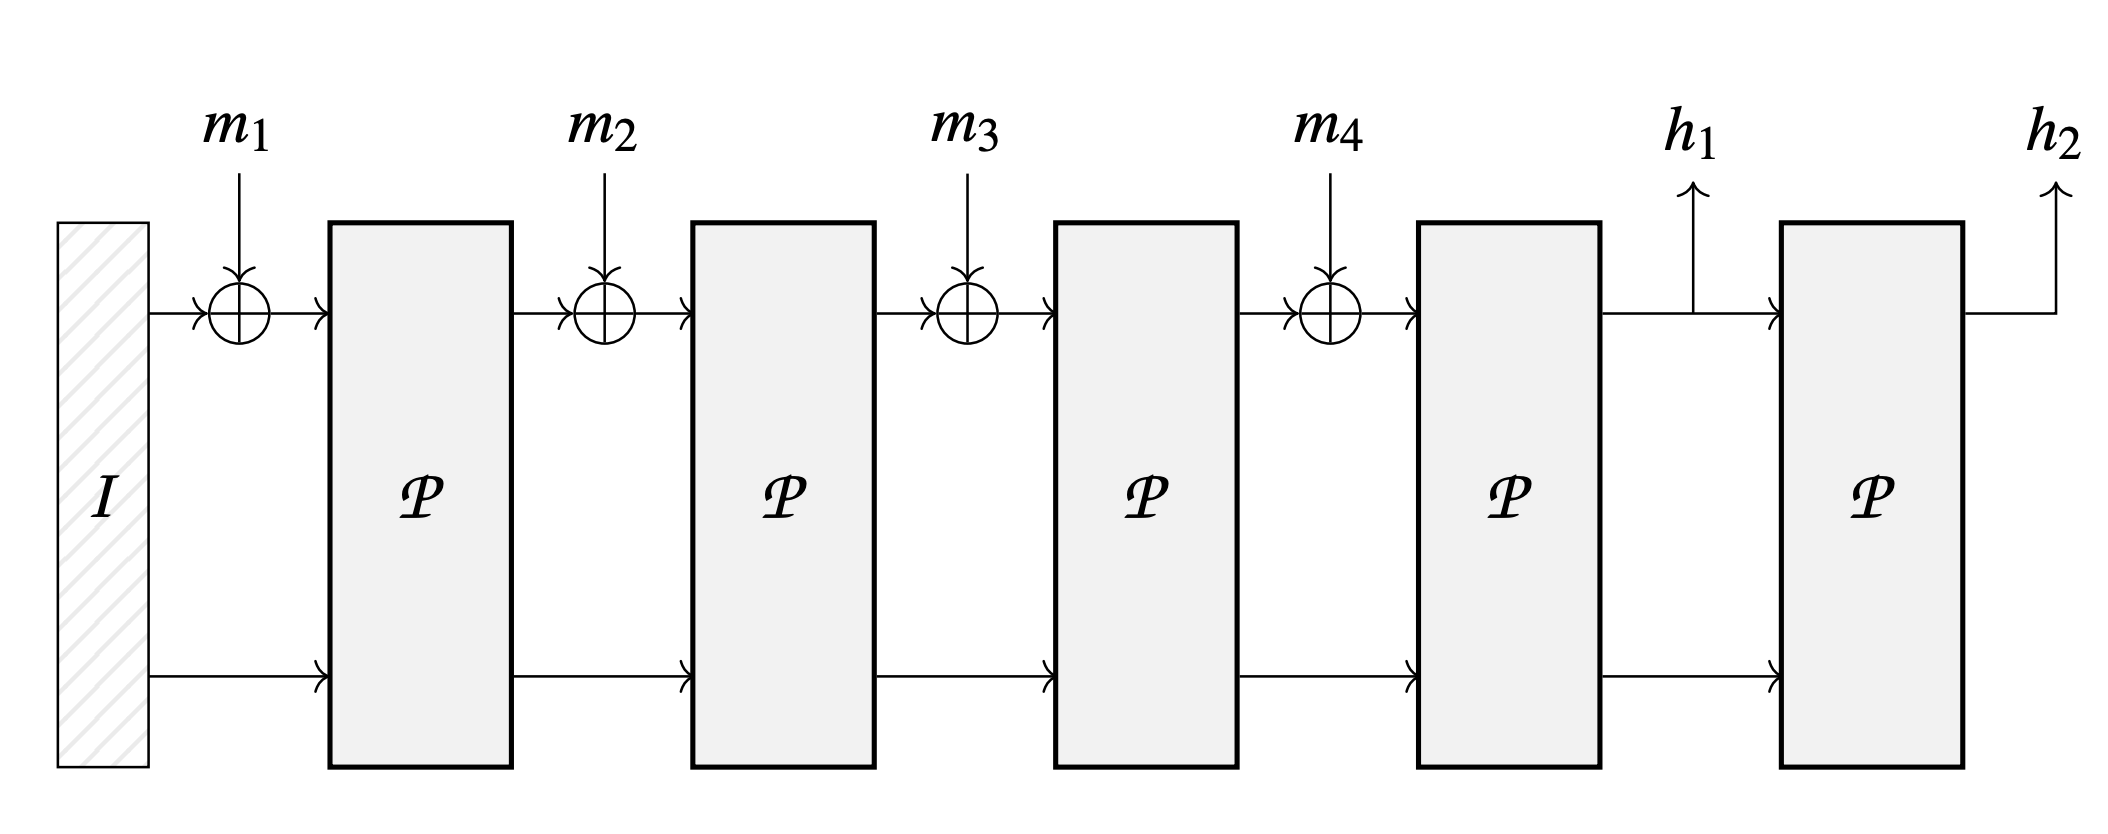
\includegraphics[width=1\textwidth]{sponge.png}
            \caption{Une fonction de hachage en éponge}
        \end{figure}
    \end{column}

    \begin{column}{0.5\textwidth}
        \begin{figure}[h!]
            \centering
            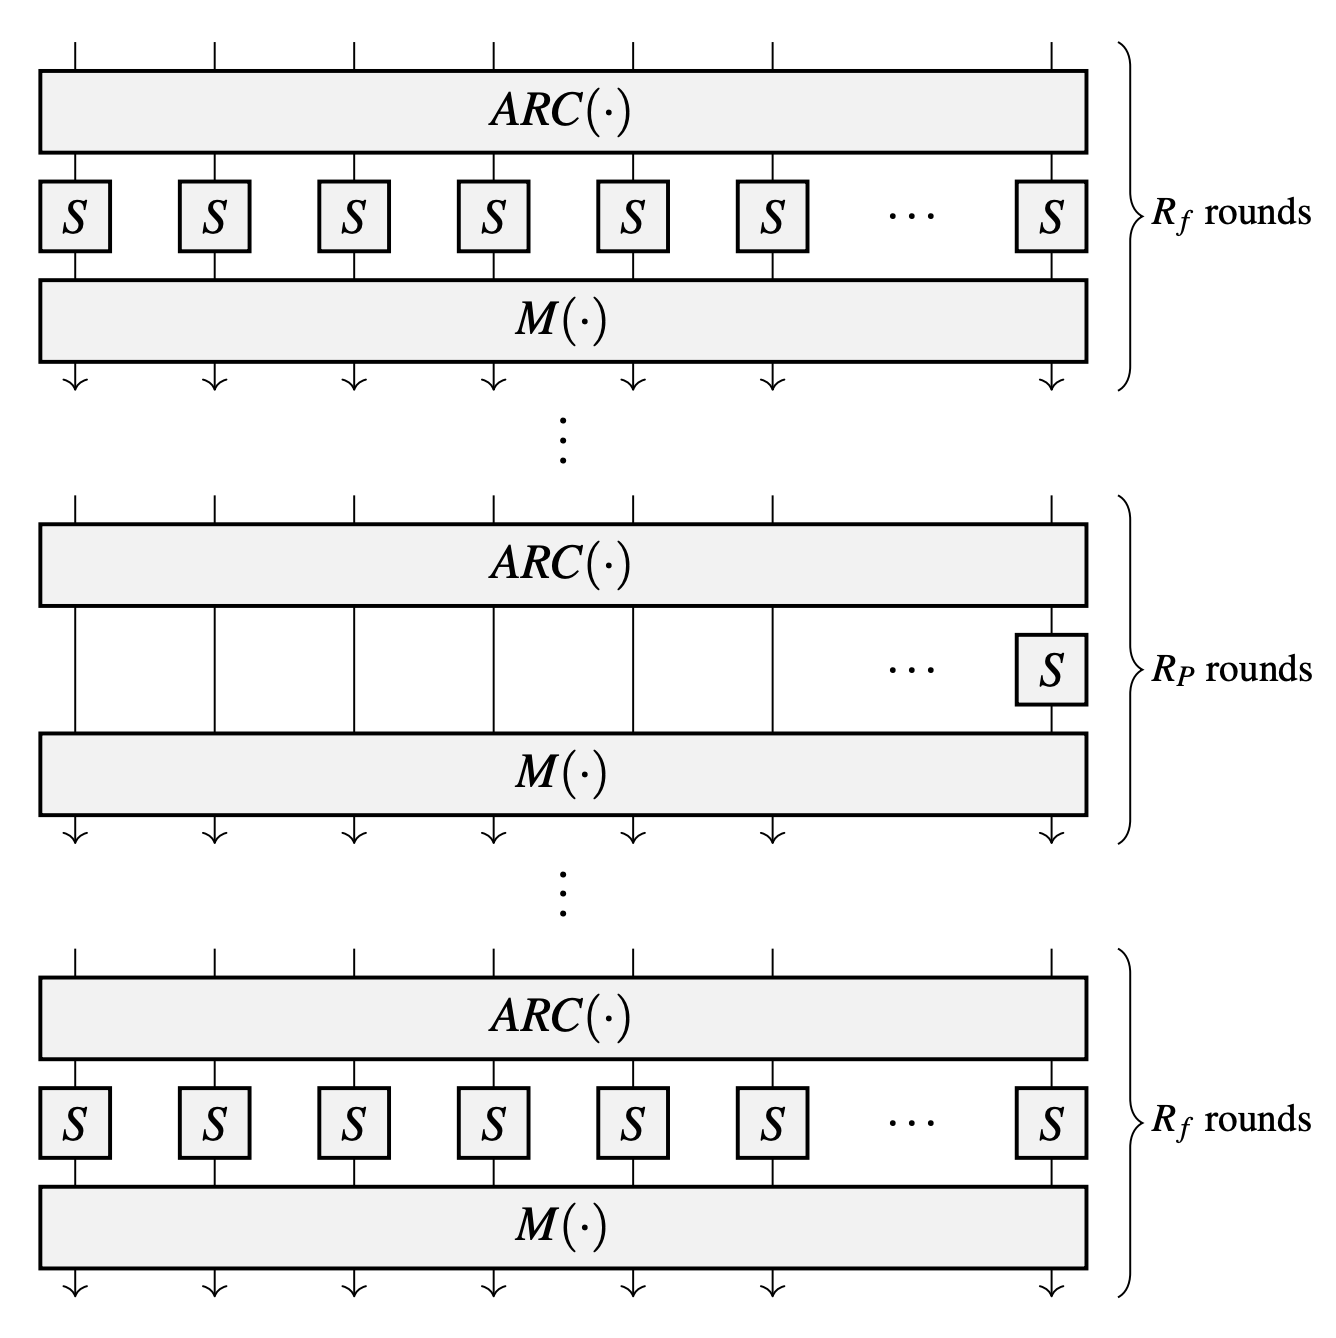
\includegraphics[width=0.5\textwidth]{perm.png}
            \caption{La permutation poséidon}
        \end{figure}
    \end{column}
\end{columns}

\end{frame}

\AtBeginSection[]
{
  \begin{frame}
    \frametitle{Sommaire}
    \tableofcontents[currentsection]
  \end{frame}
}
\section{Conclusion}

\begin{frame}
\frametitle{Annexe: Avancement}
\begin{enumerate}
    \item 01-02/25: Lecture des papiers sur Cairo, STARK et FRI
    \item 03/25: STARK 101
    \item 04-06/25: Polynômes et utilitaires en Ocaml
    \item 09/25: Idée AFD et premier prototype d'AIR
    \item 11/25: Prototype fini sans ZK
    \item 01/26: Fini la rédaction d'articles sur ce premier prototype
    \item 02/26: Fini prototype avec le hash
    \item 02/26: Gros problème
\end{enumerate}
\end{frame}
\begin{frame}
\frametitle{Annexe: Code}
\begin{figure}[h!]
  \centering
  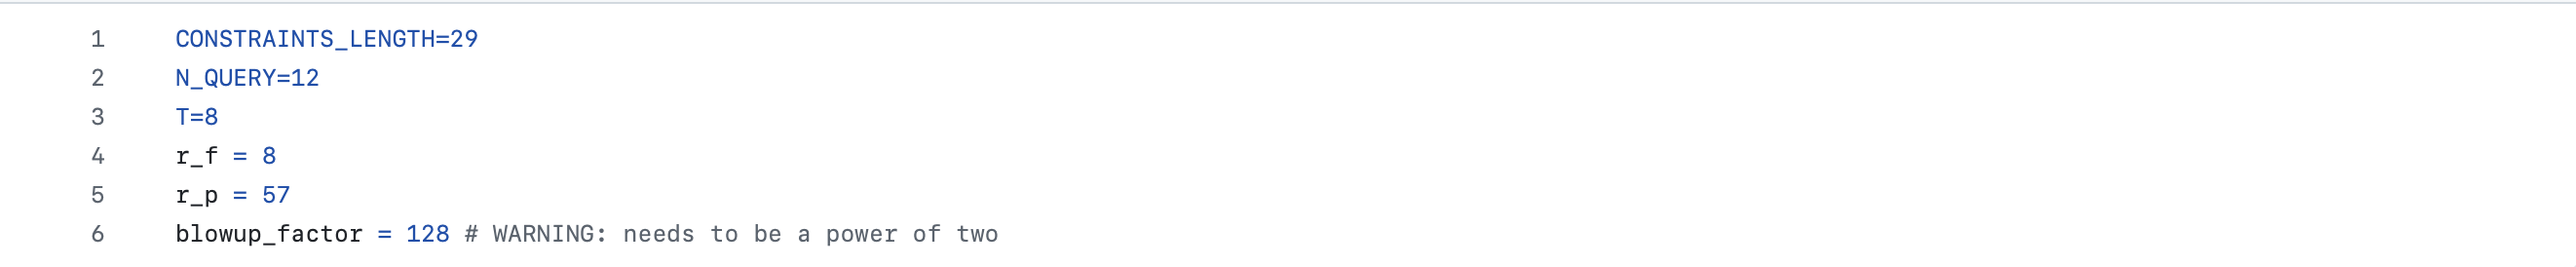
\includegraphics[width=0.8\textwidth]{1.png}
\end{figure}
\end{frame}
\begin{frame}
\frametitle{Annexe: Code}
\begin{figure}[h!]
  \centering
  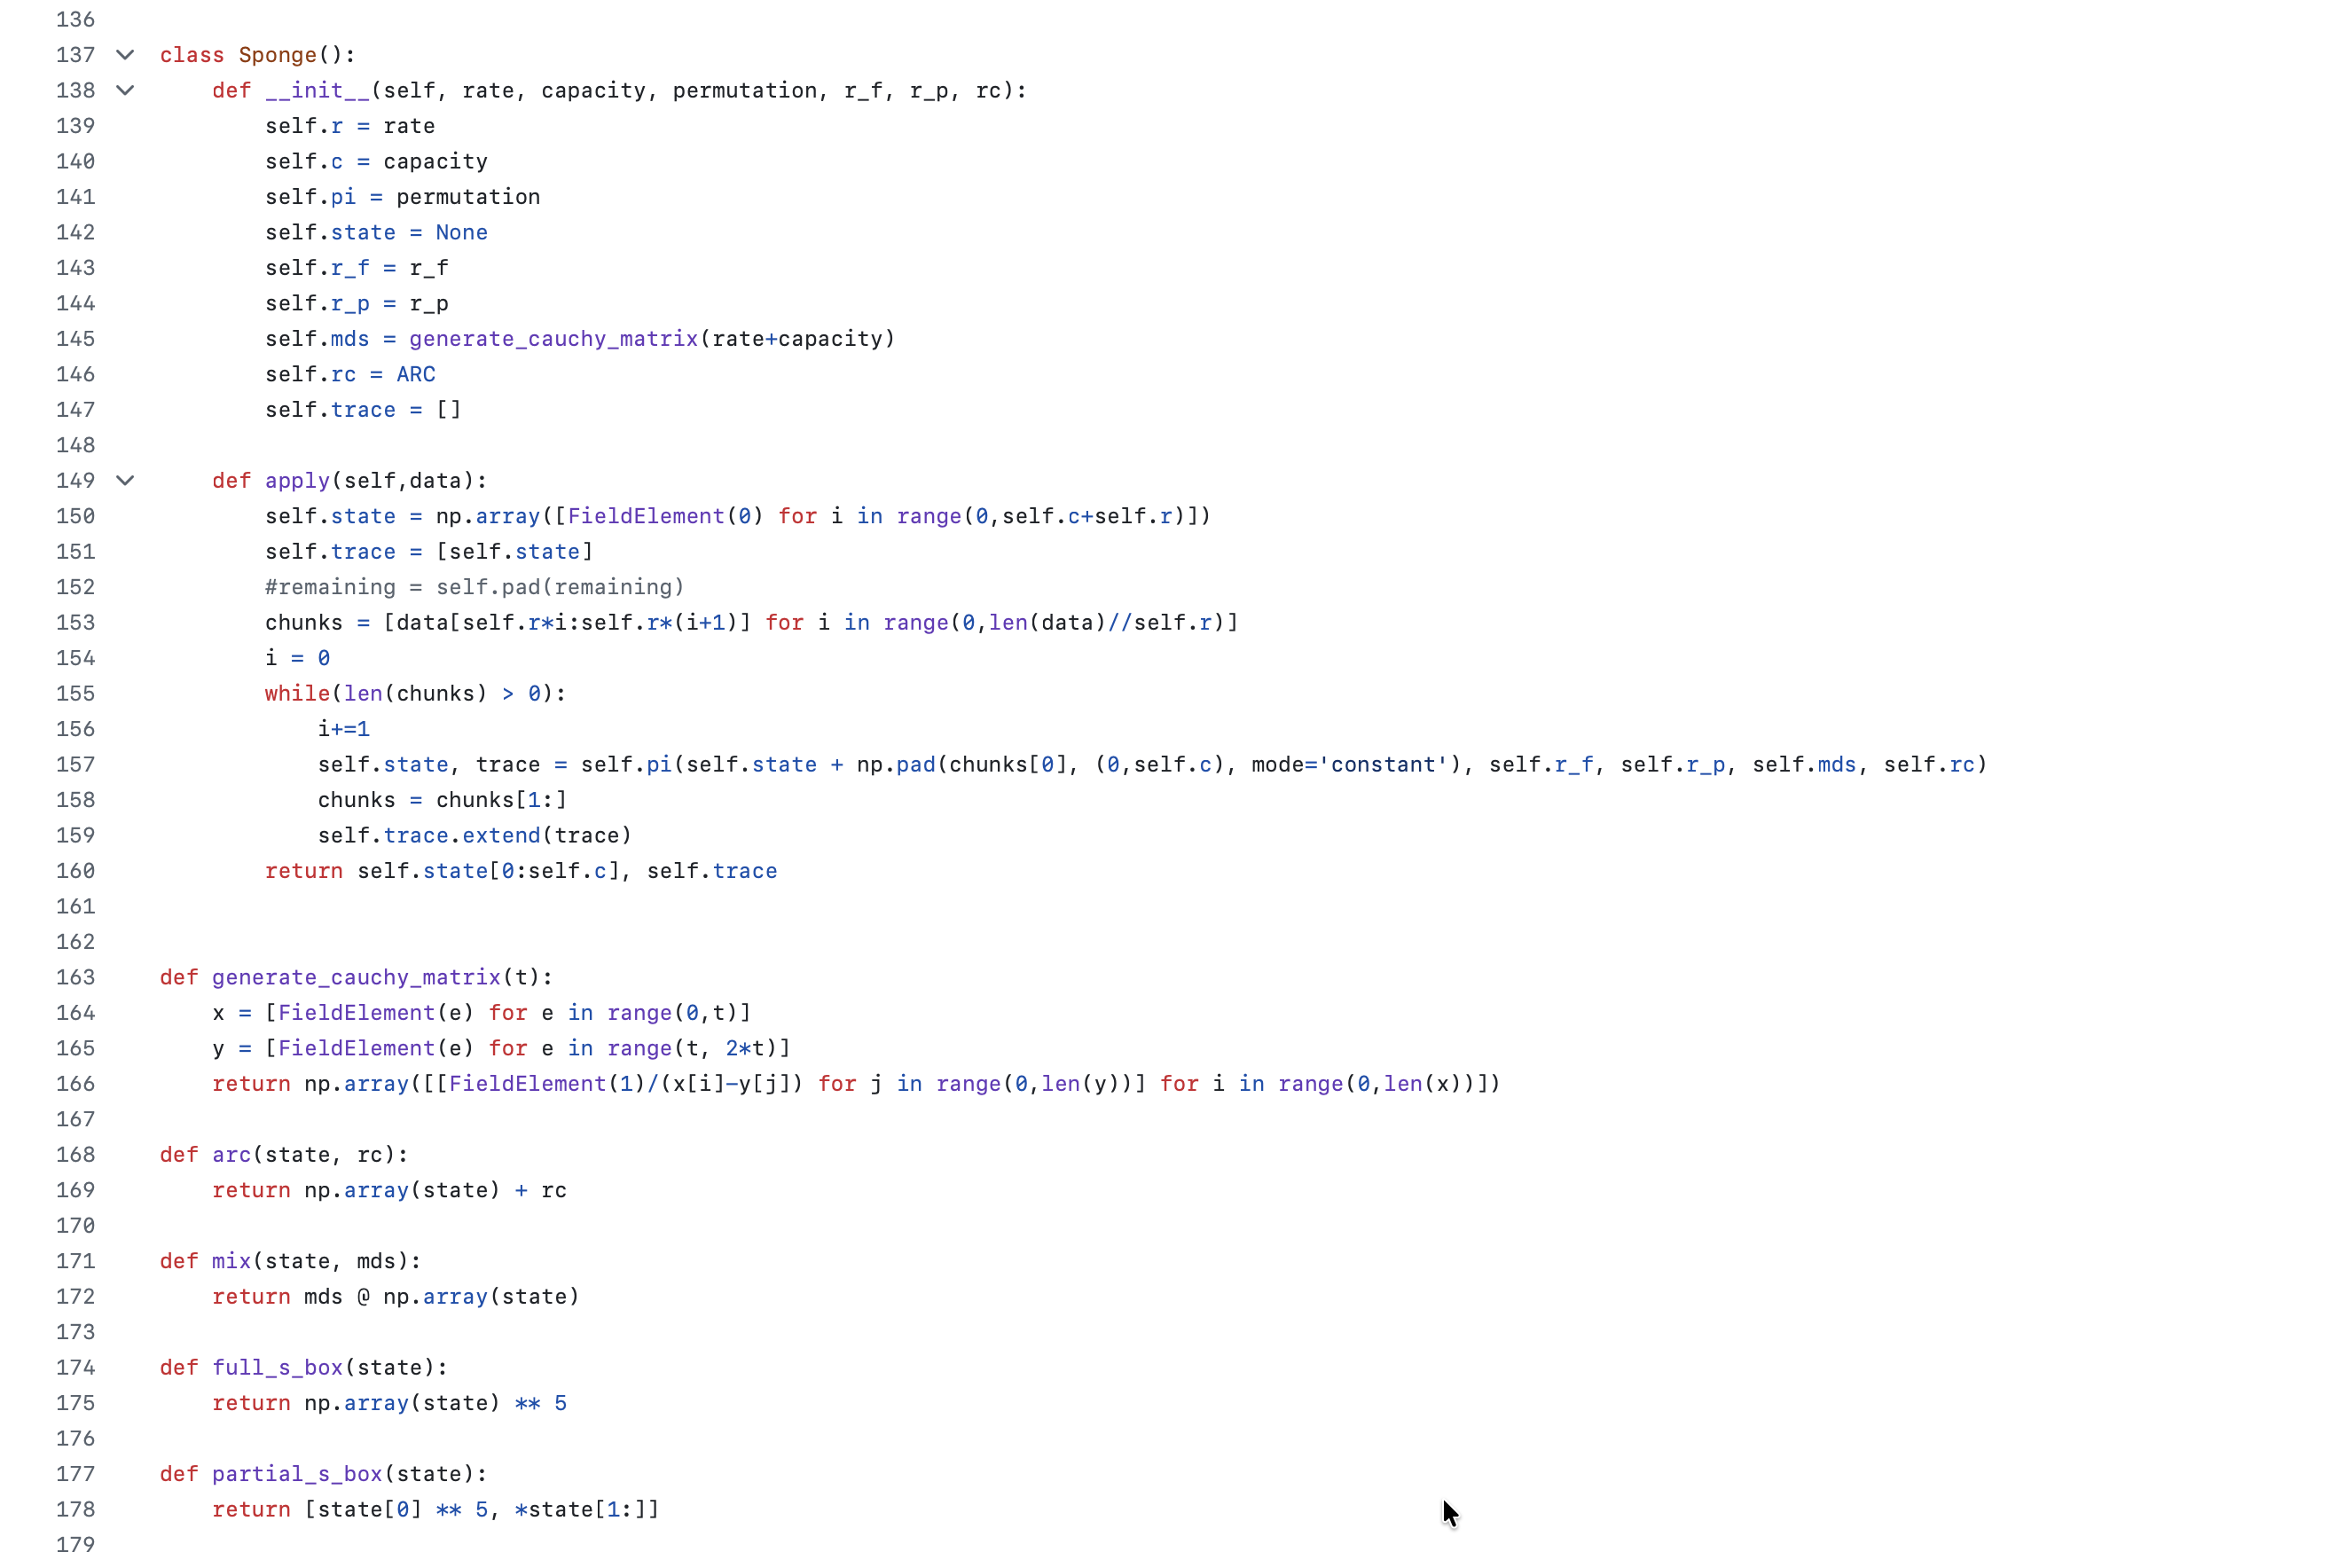
\includegraphics[width=0.8\textwidth]{2.png}
\end{figure}
\end{frame}
\begin{frame}
\frametitle{Annexe: Code}
\begin{figure}[h!]
  \centering
  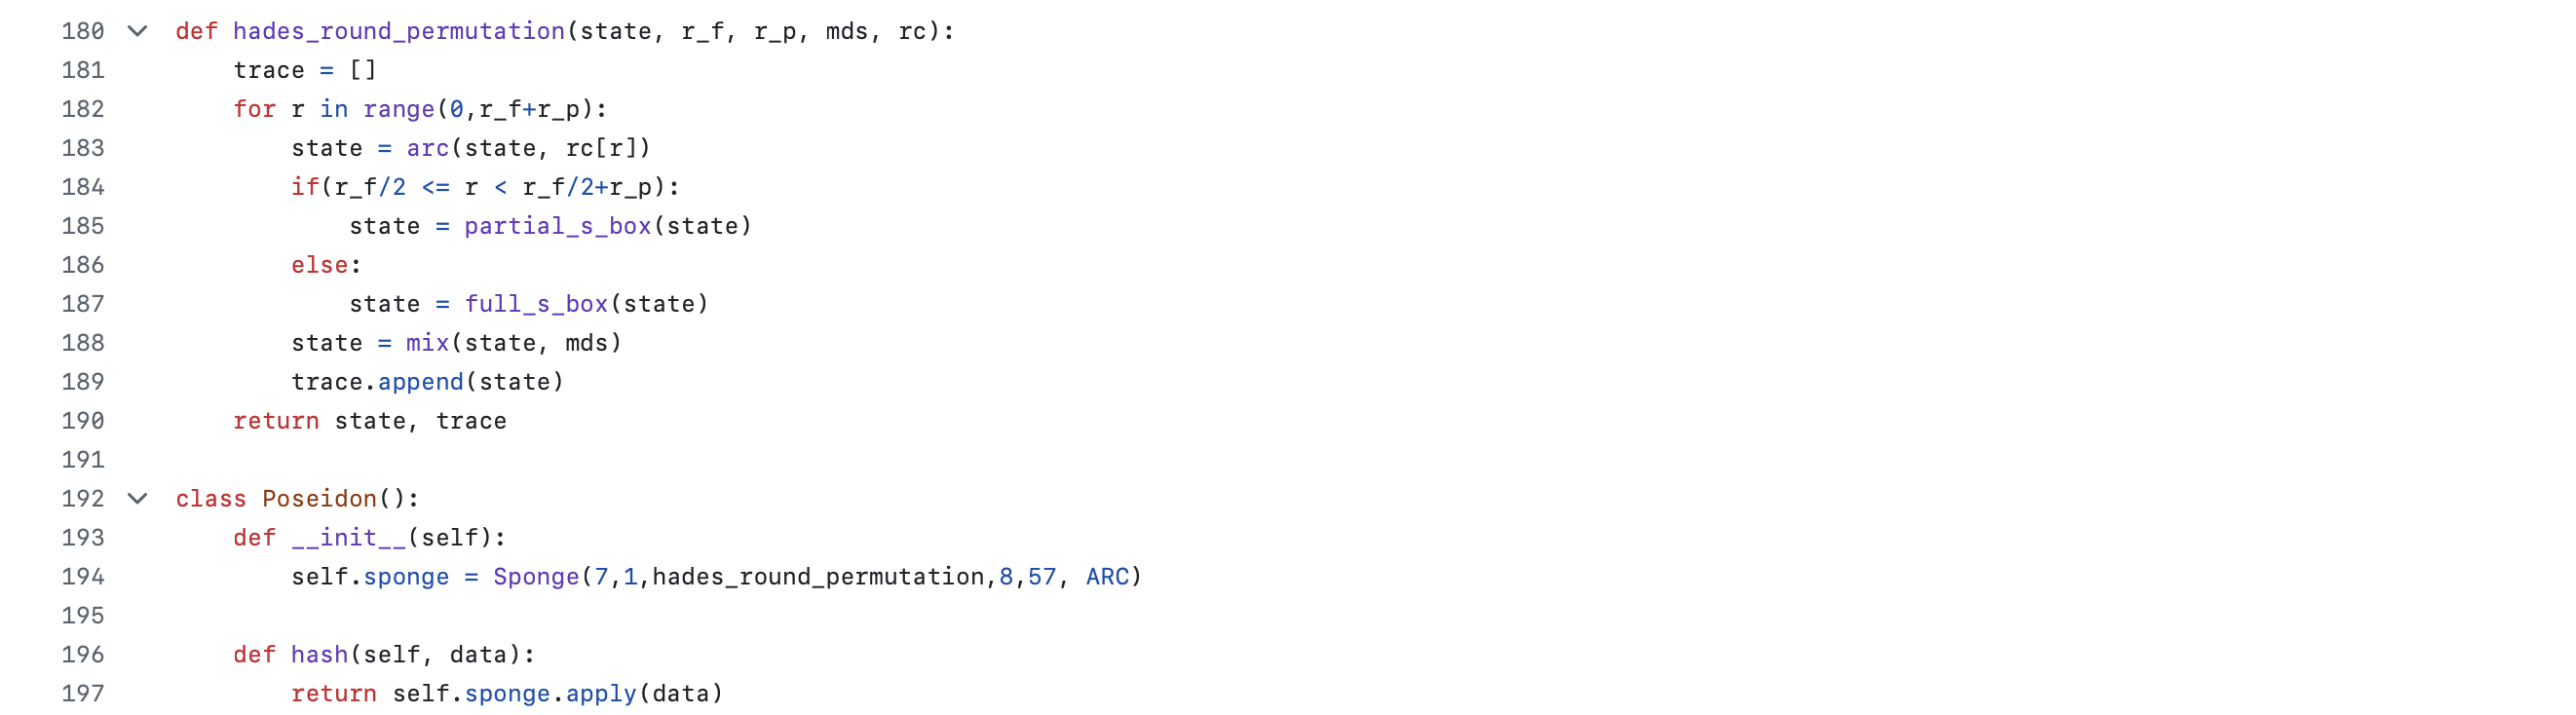
\includegraphics[width=0.8\textwidth]{3.png}
\end{figure}
\end{frame}
\begin{frame}
\frametitle{Annexe: Code}
\begin{figure}[h!]
  \centering
  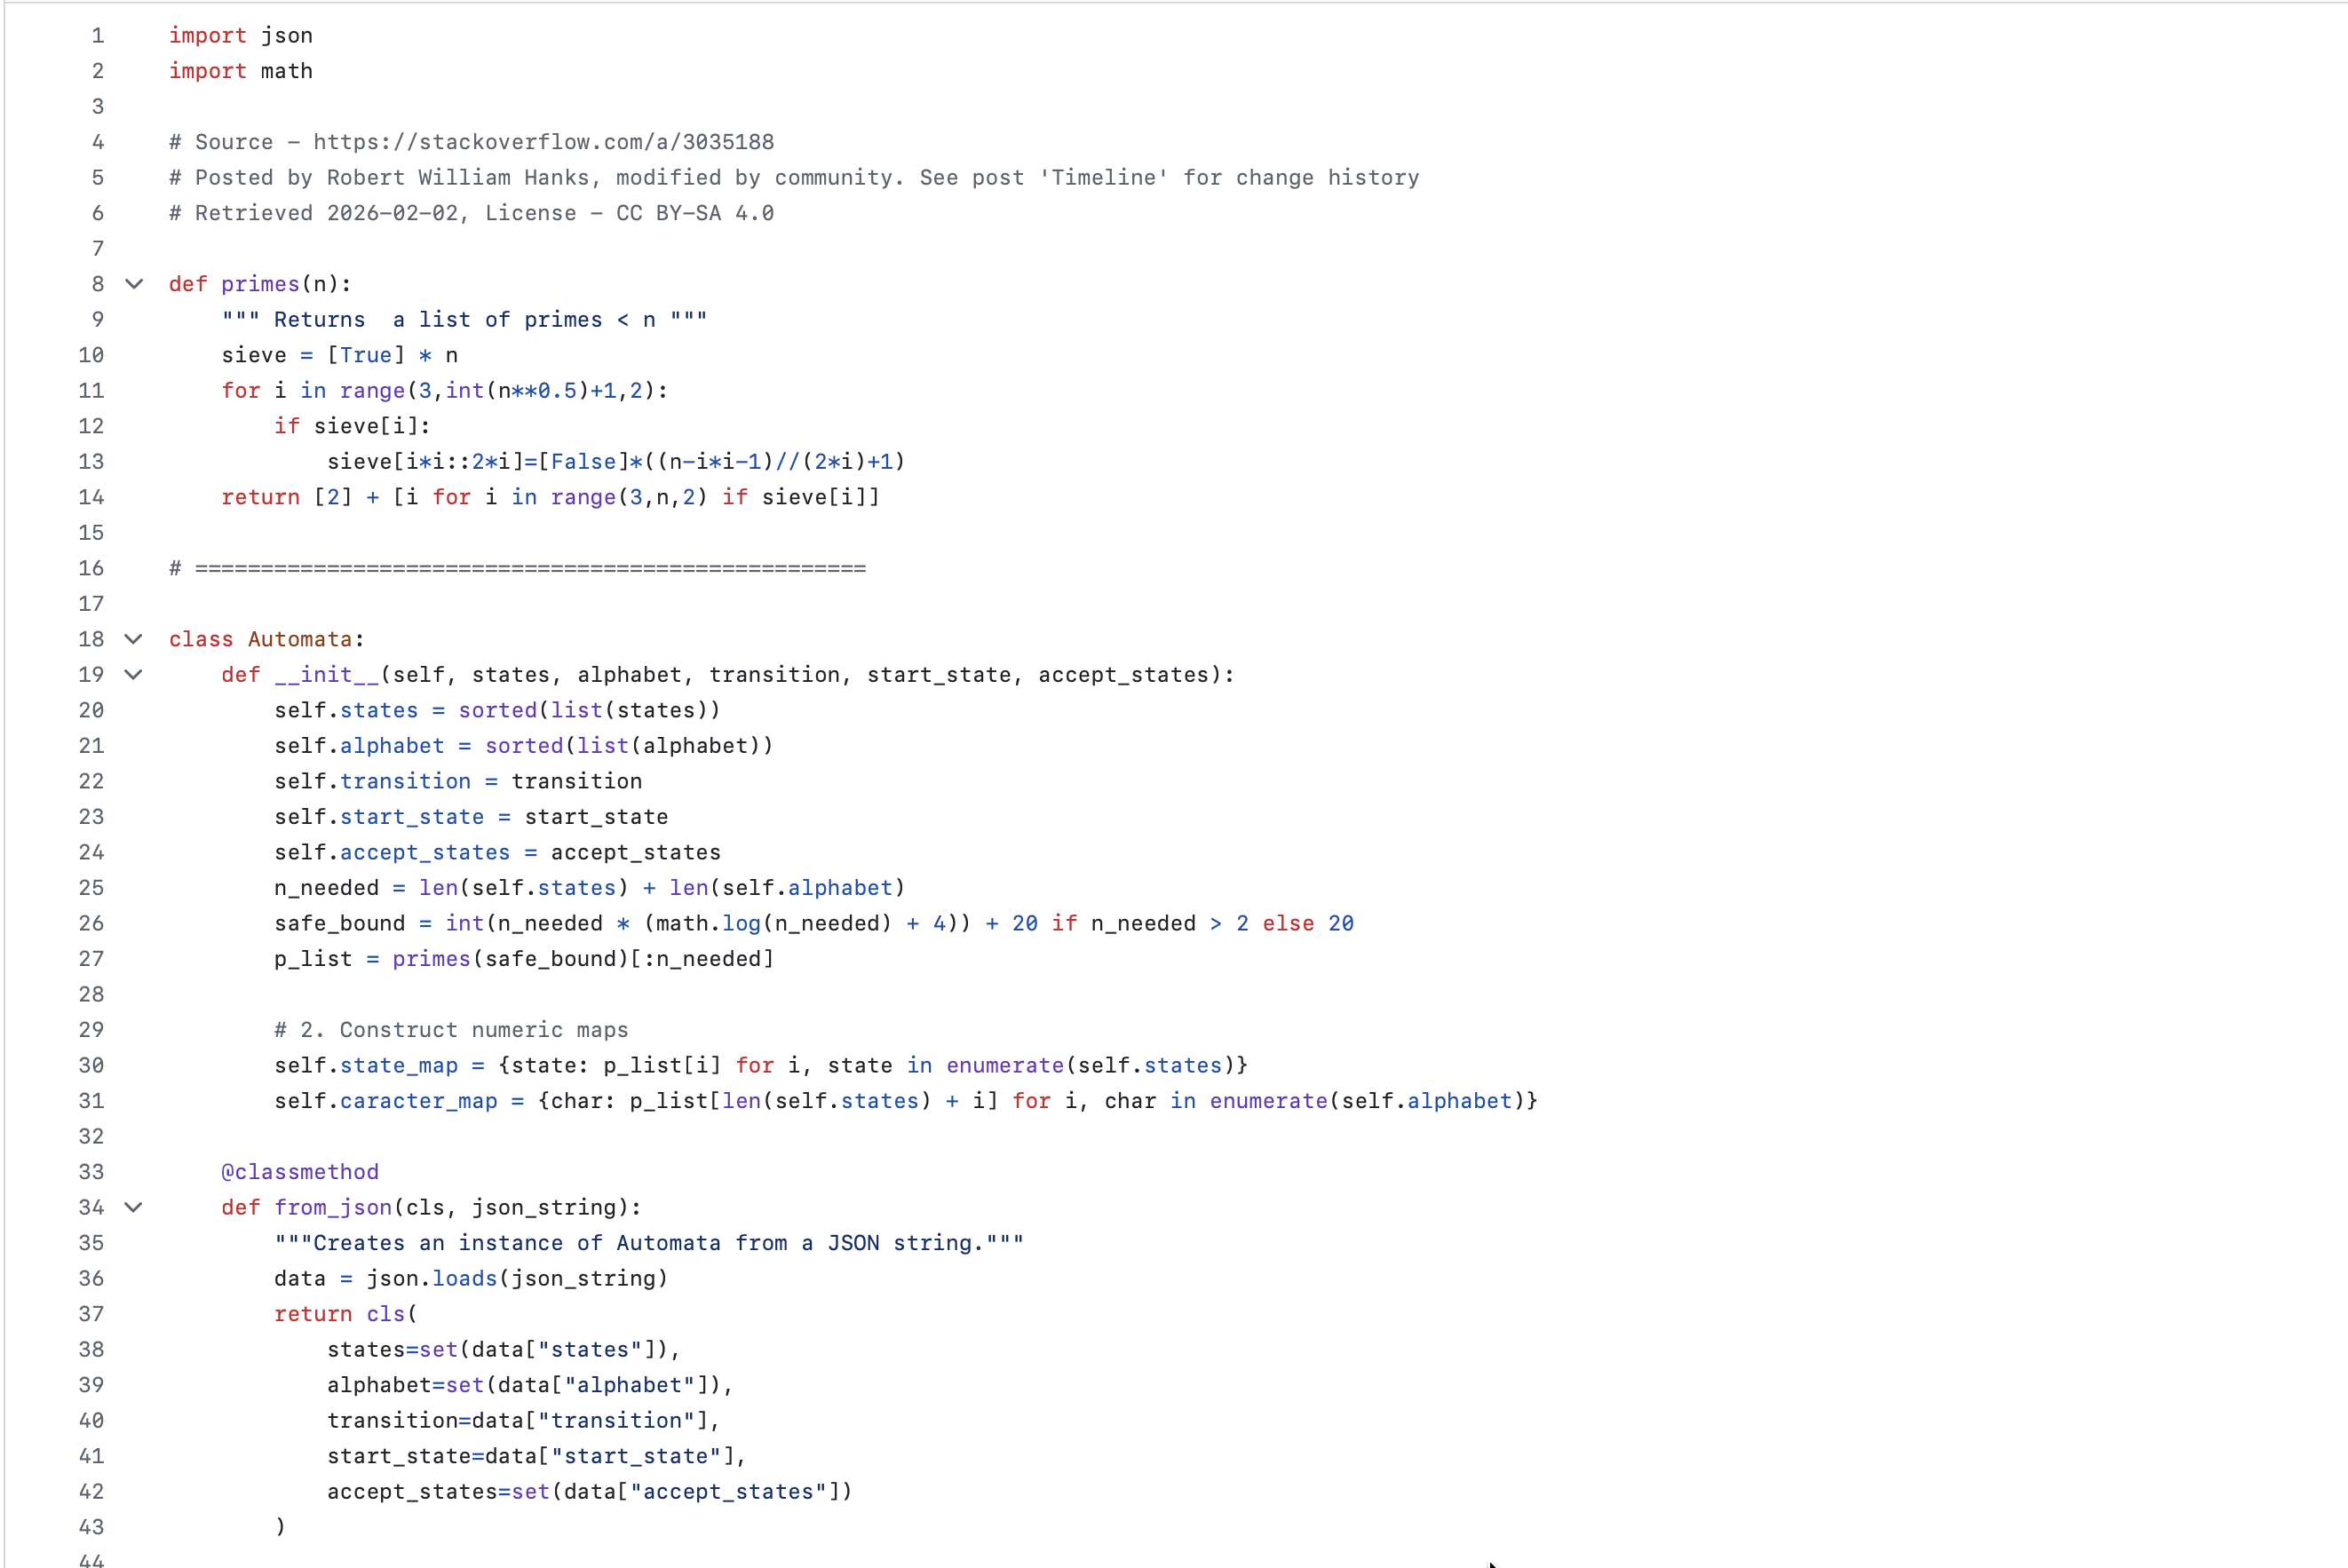
\includegraphics[width=0.8\textwidth]{4.png}
\end{figure}
\end{frame}
\begin{frame}
\frametitle{Annexe: Code}
\begin{figure}[h!]
  \centering
  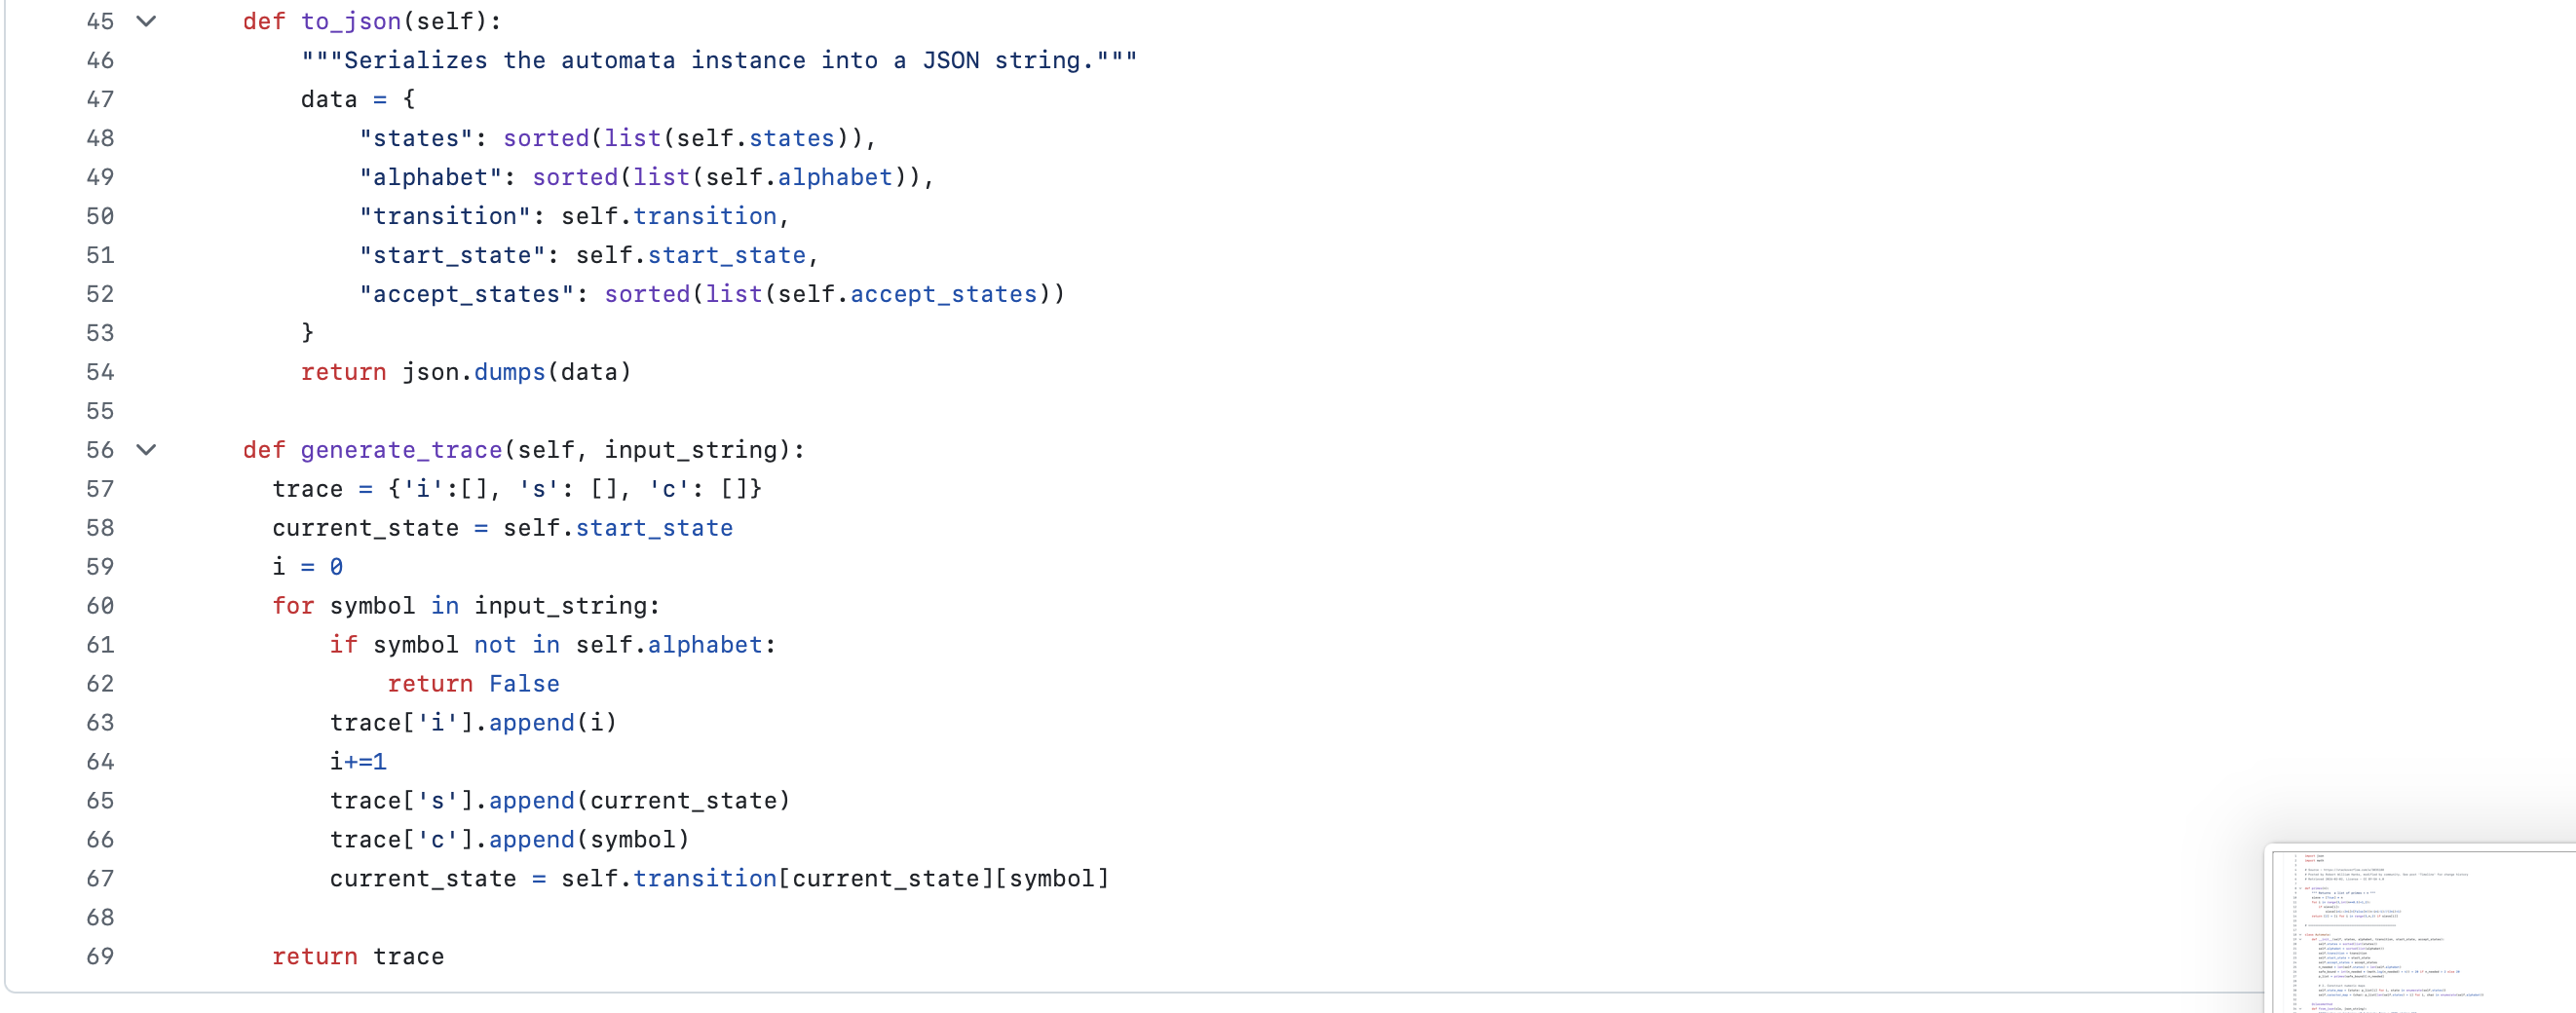
\includegraphics[width=0.8\textwidth]{5.png}
\end{figure}
\end{frame}
\begin{frame}
\frametitle{Annexe: Code}
\begin{figure}[h!]
  \centering
  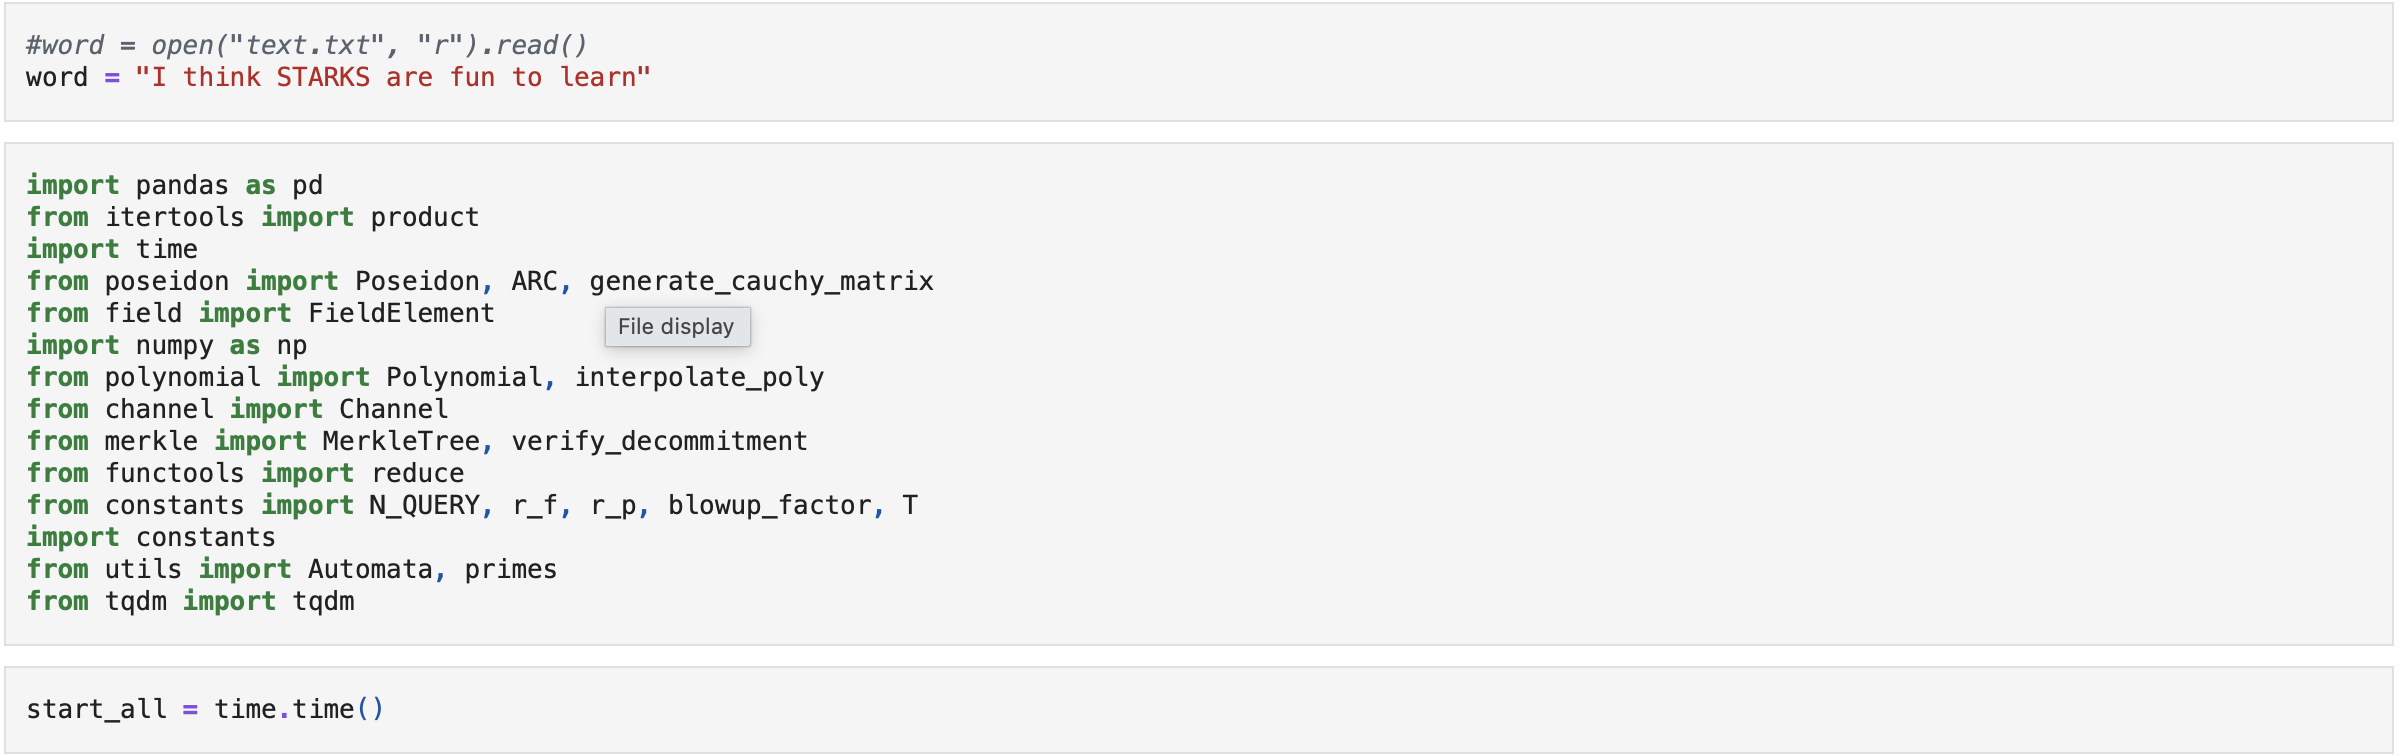
\includegraphics[width=0.8\textwidth]{6.png}
\end{figure}
\end{frame}
\begin{frame}
\frametitle{Annexe: Code}
\begin{figure}[h!]
  \centering
  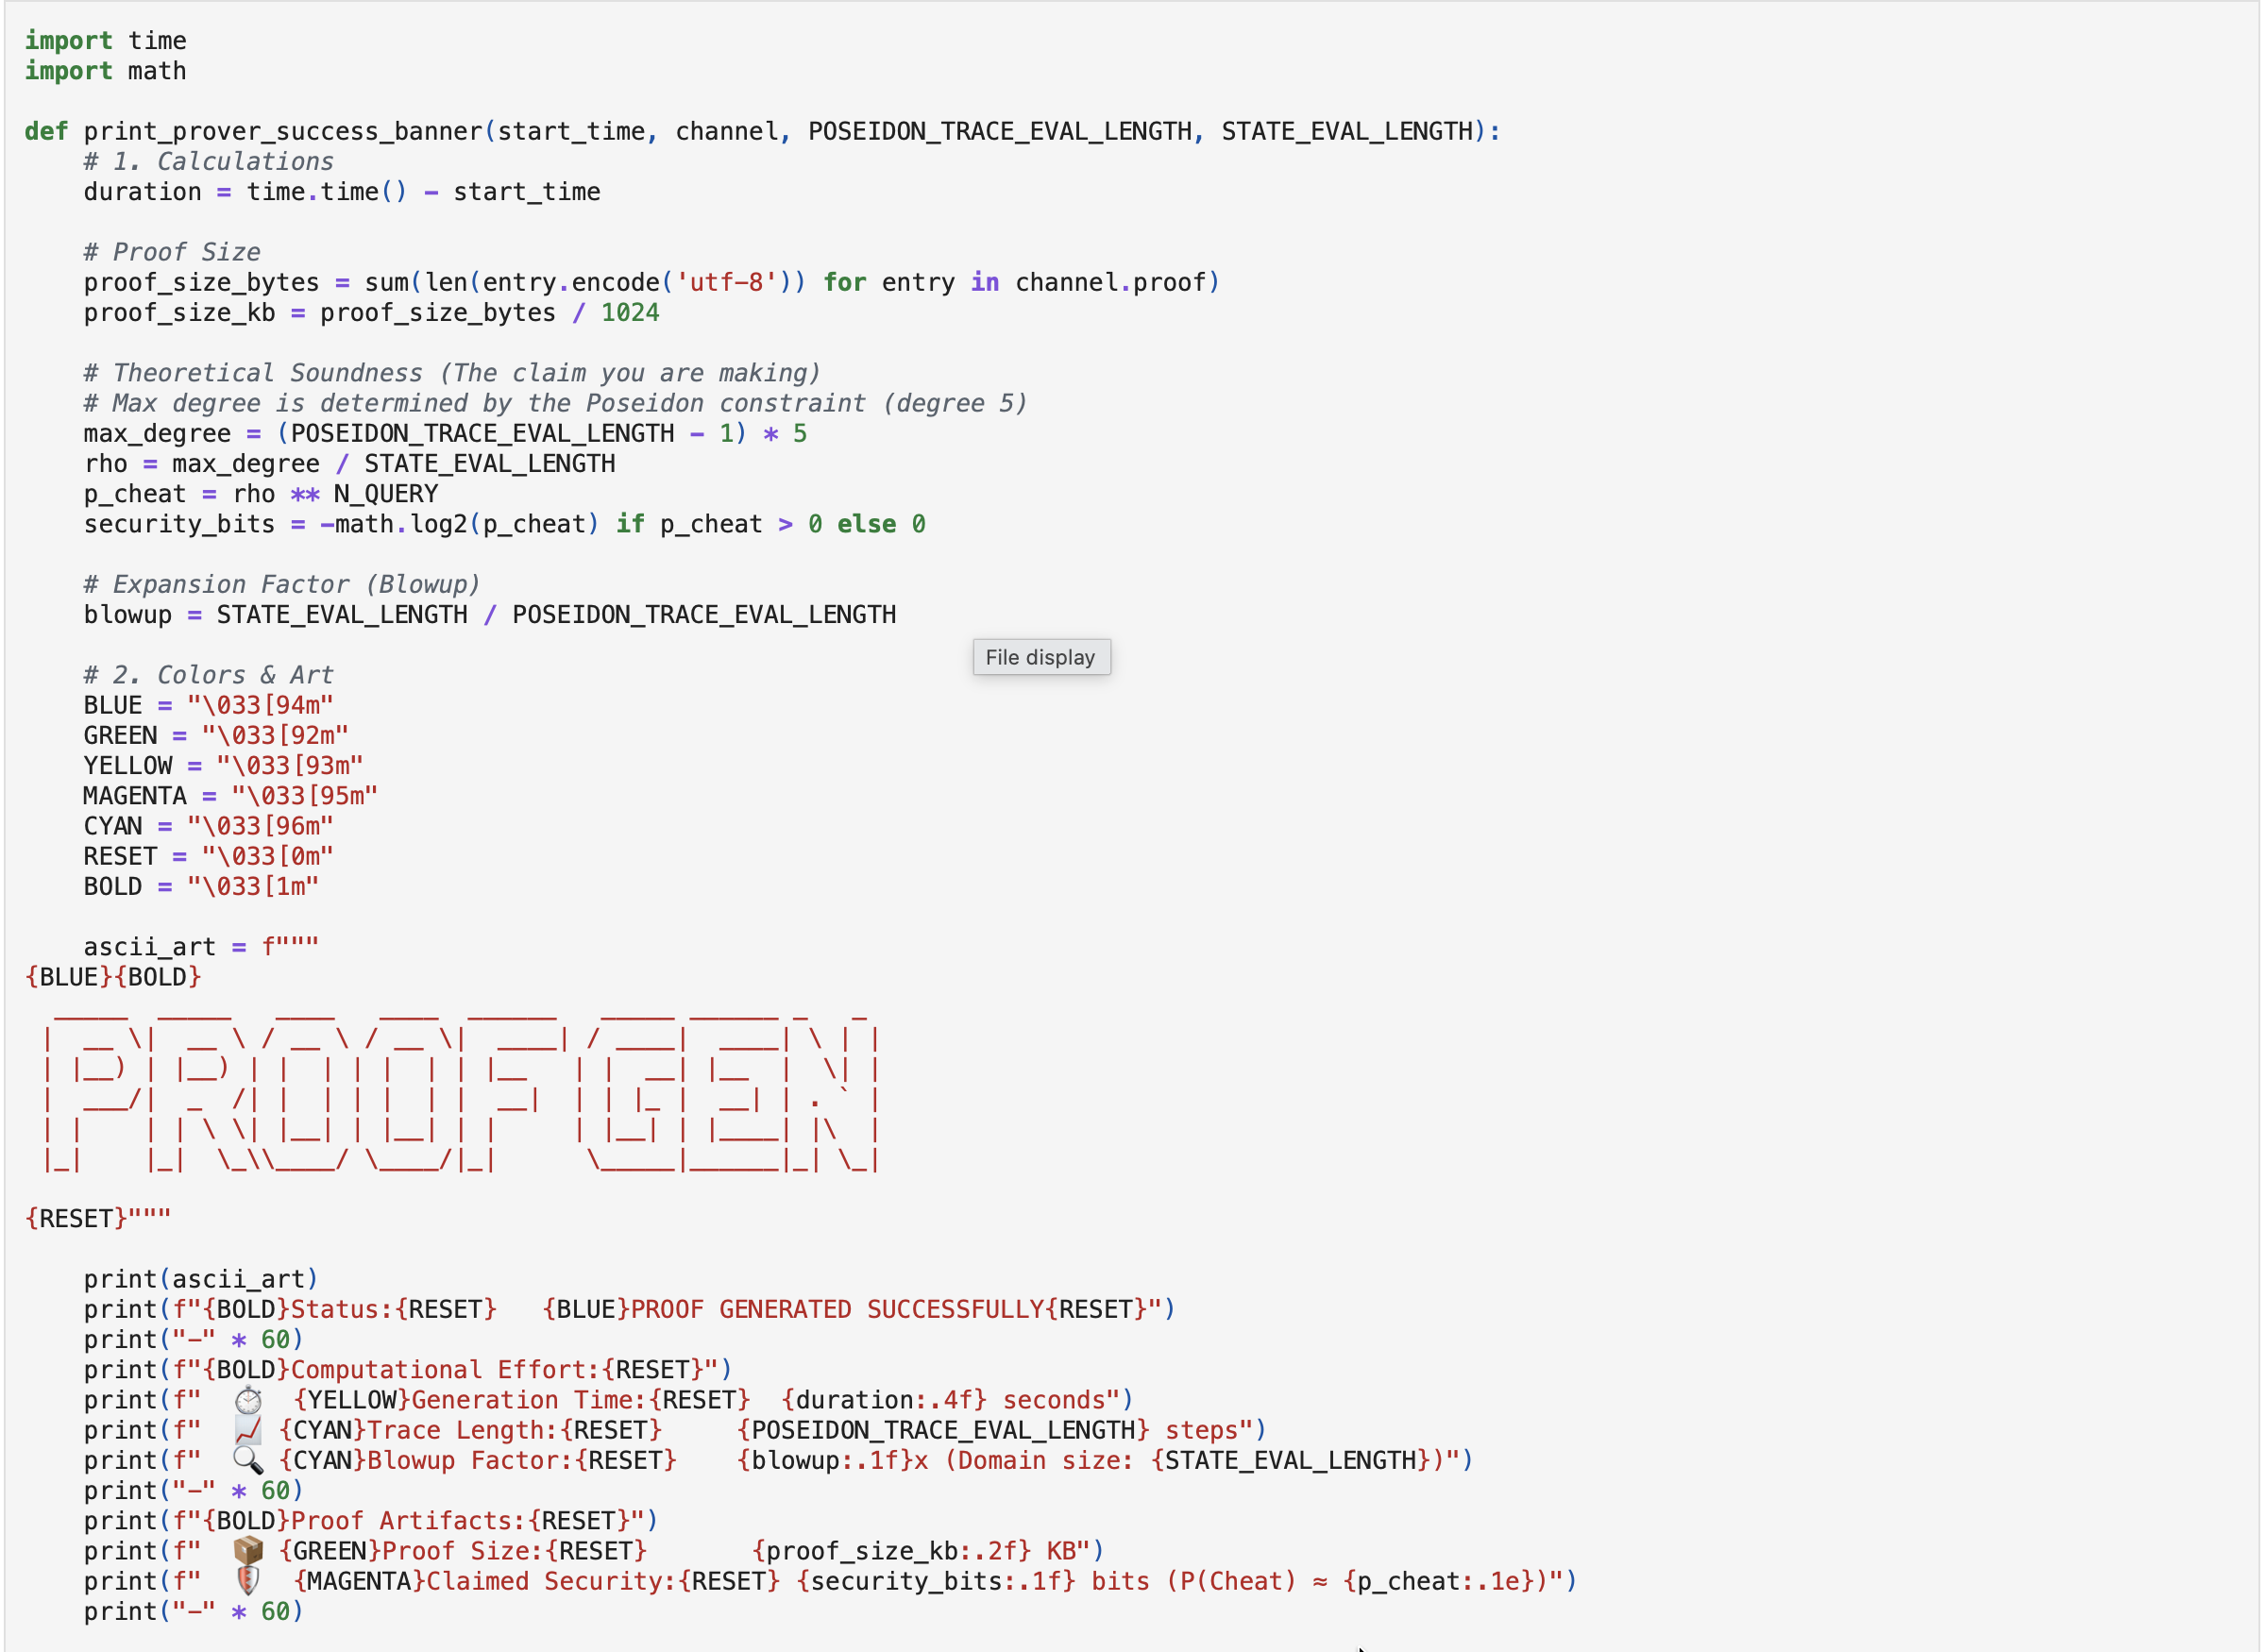
\includegraphics[width=0.8\textwidth]{7.png}
\end{figure}
\end{frame}
\begin{frame}
\frametitle{Annexe: Code}
\begin{figure}[h!]
  \centering
  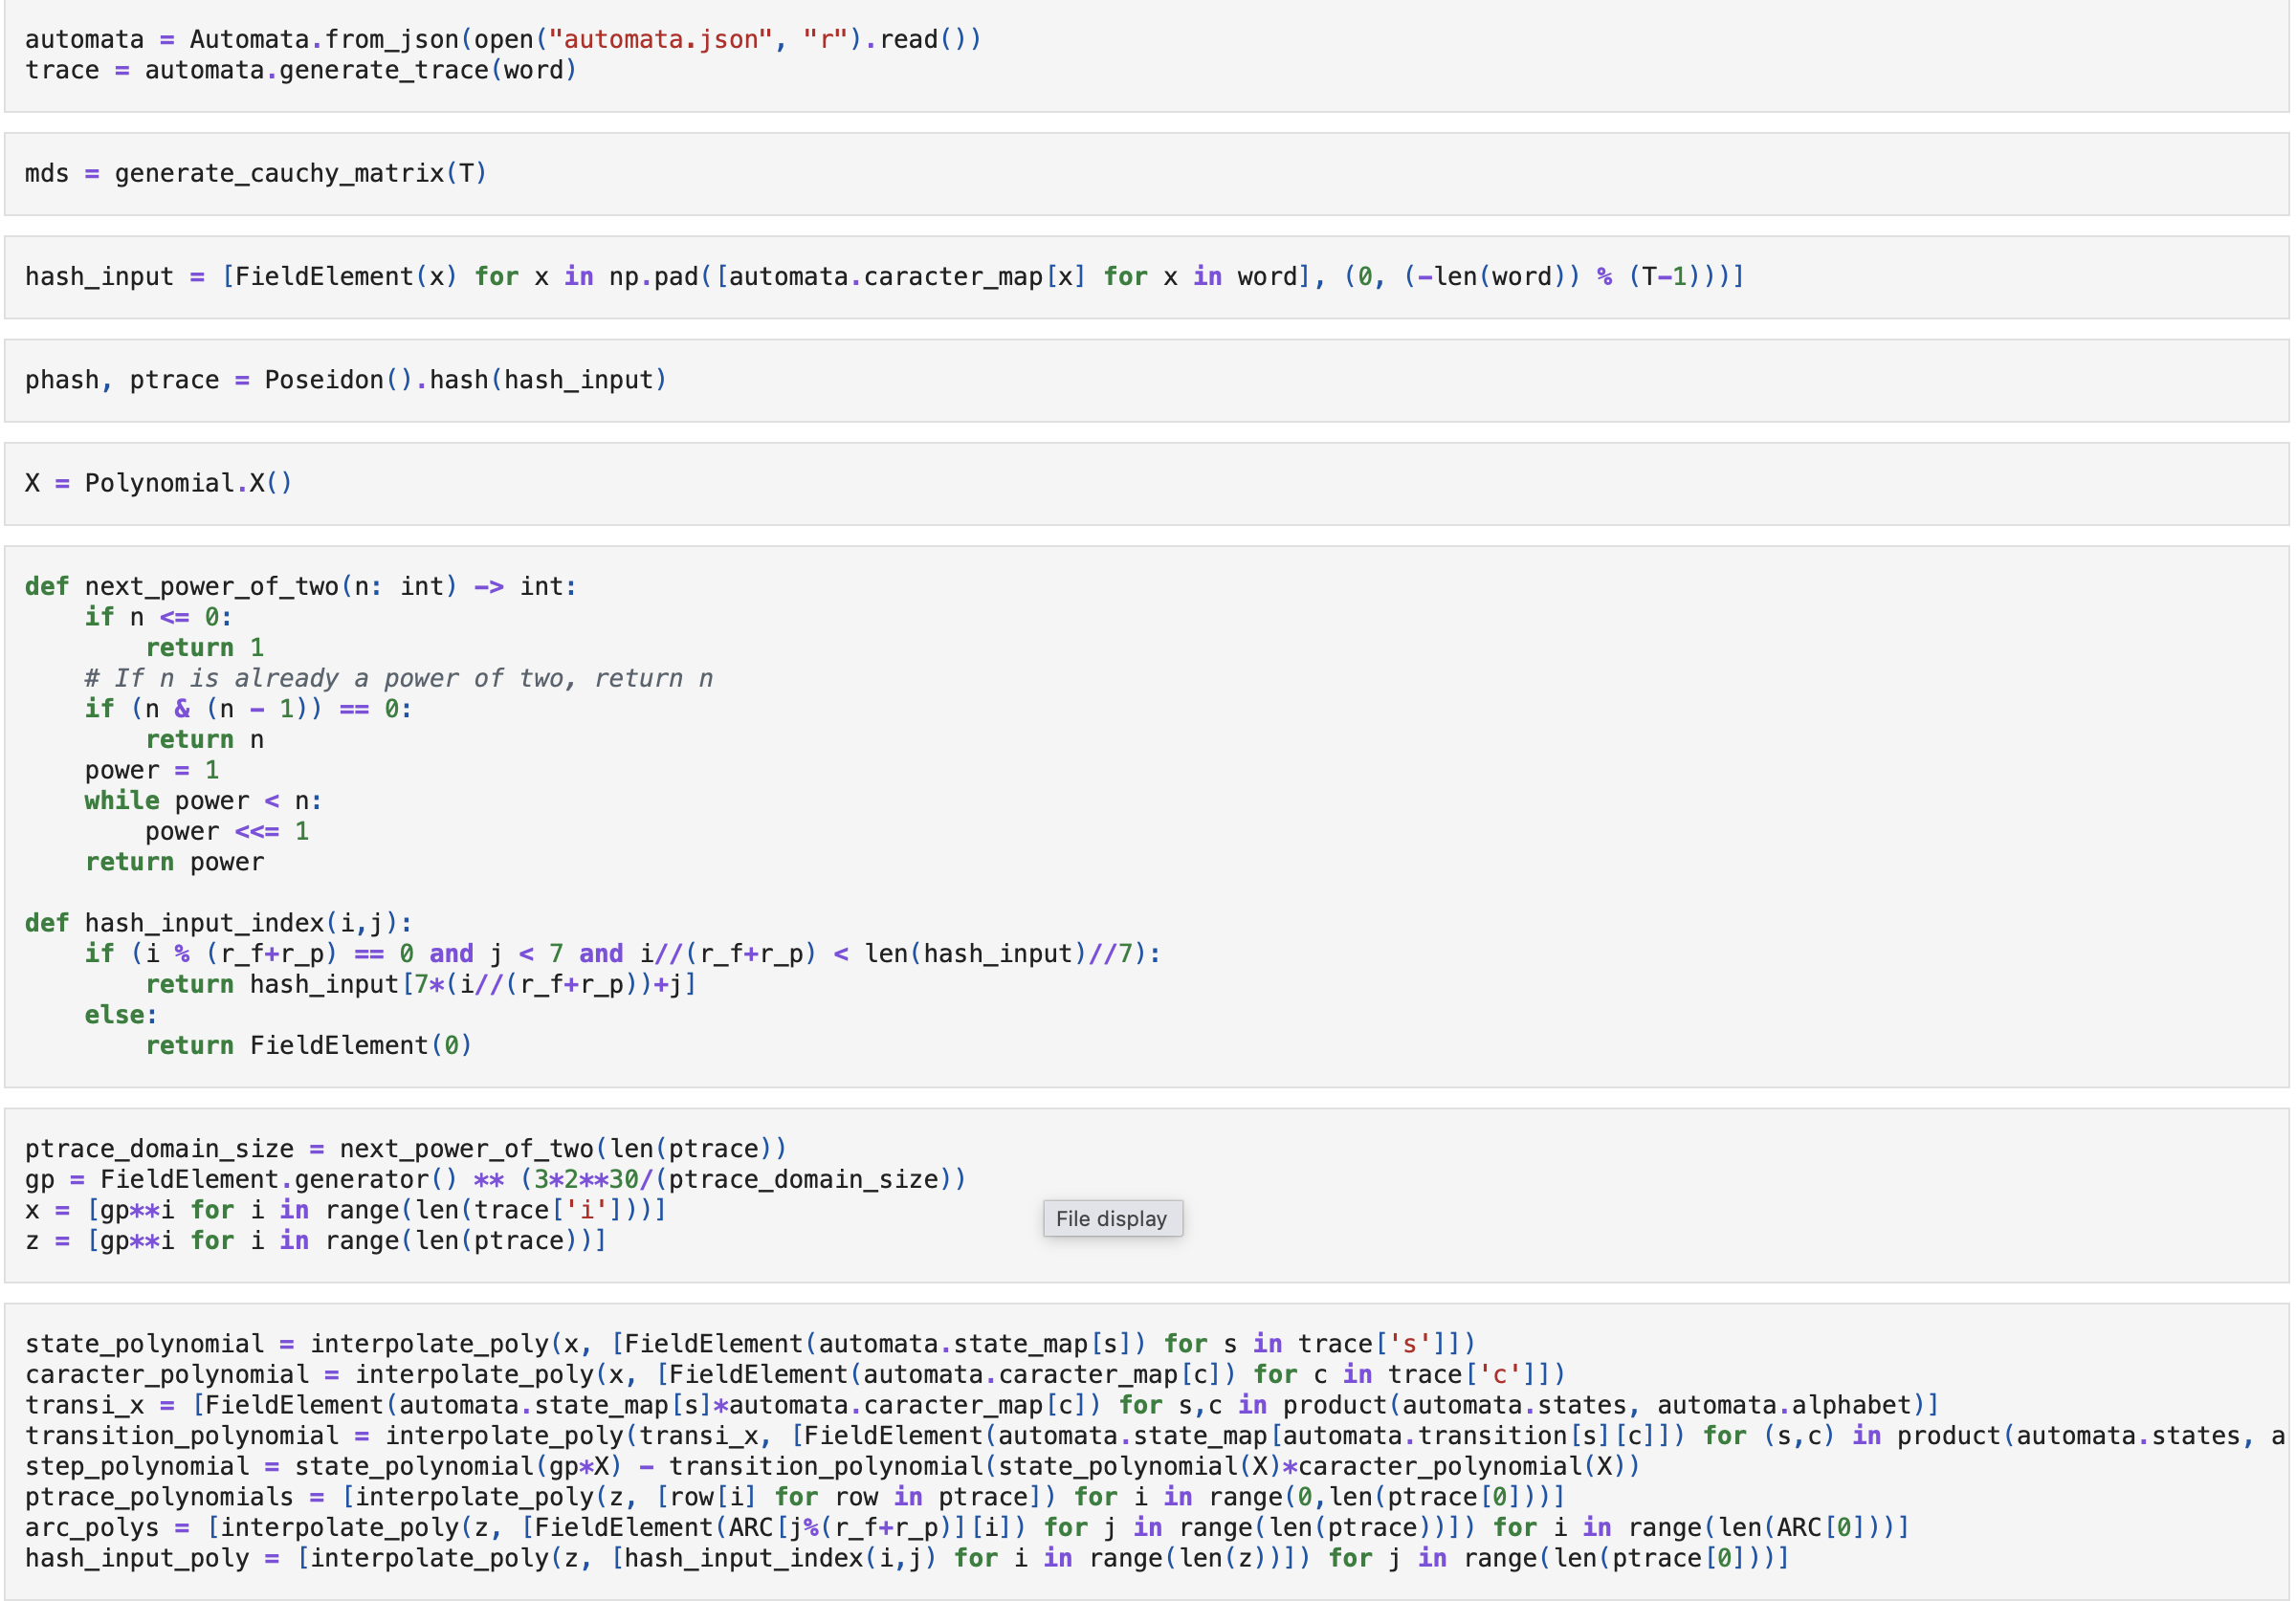
\includegraphics[width=0.8\textwidth]{8.png}
\end{figure}
\end{frame}
\begin{frame}
\frametitle{Annexe: Code}
\begin{figure}[h!]
  \centering
  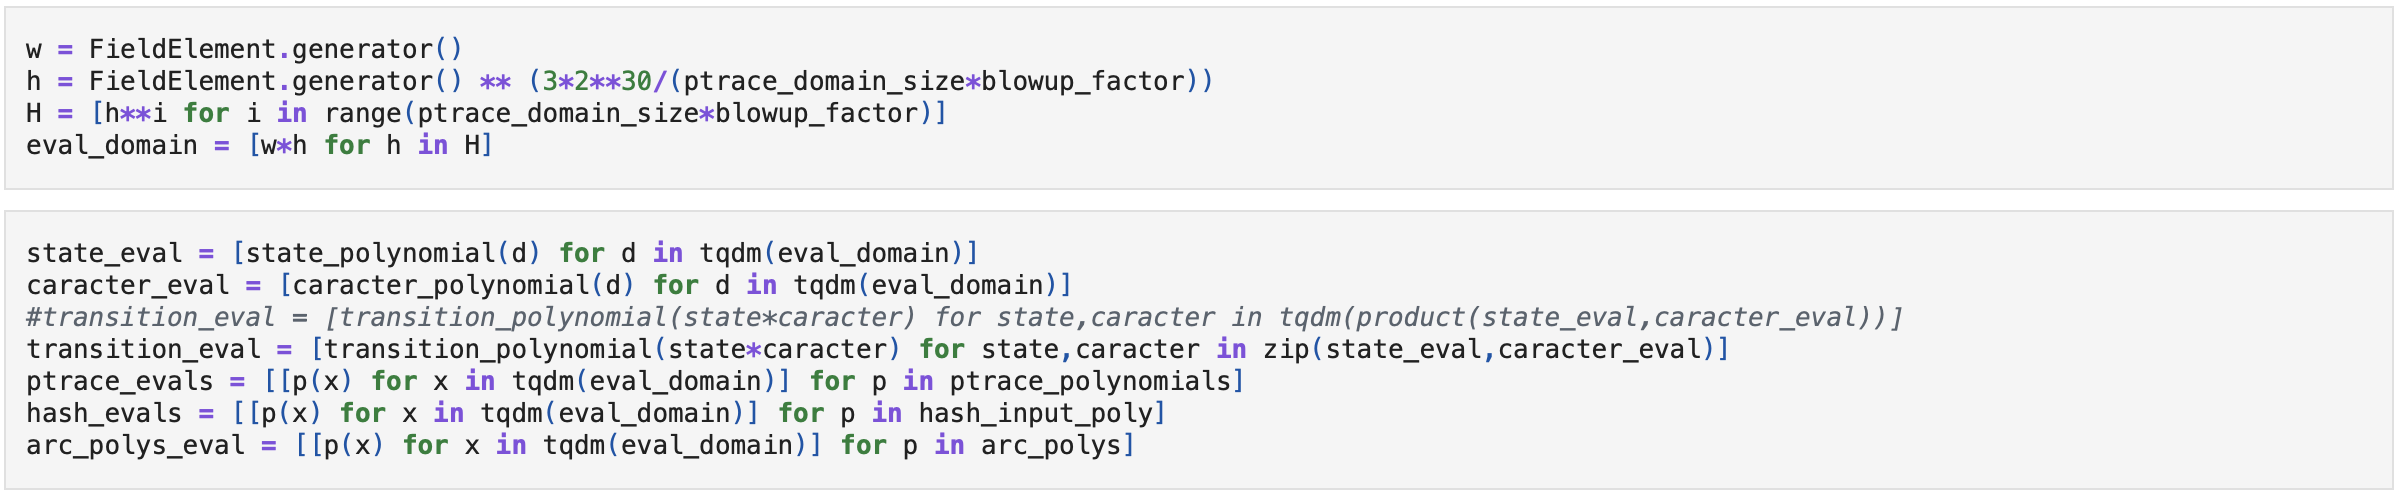
\includegraphics[width=0.8\textwidth]{9.png}
\end{figure}
\end{frame}
\begin{frame}
\frametitle{Annexe: Code}
\begin{figure}[h!]
  \centering
  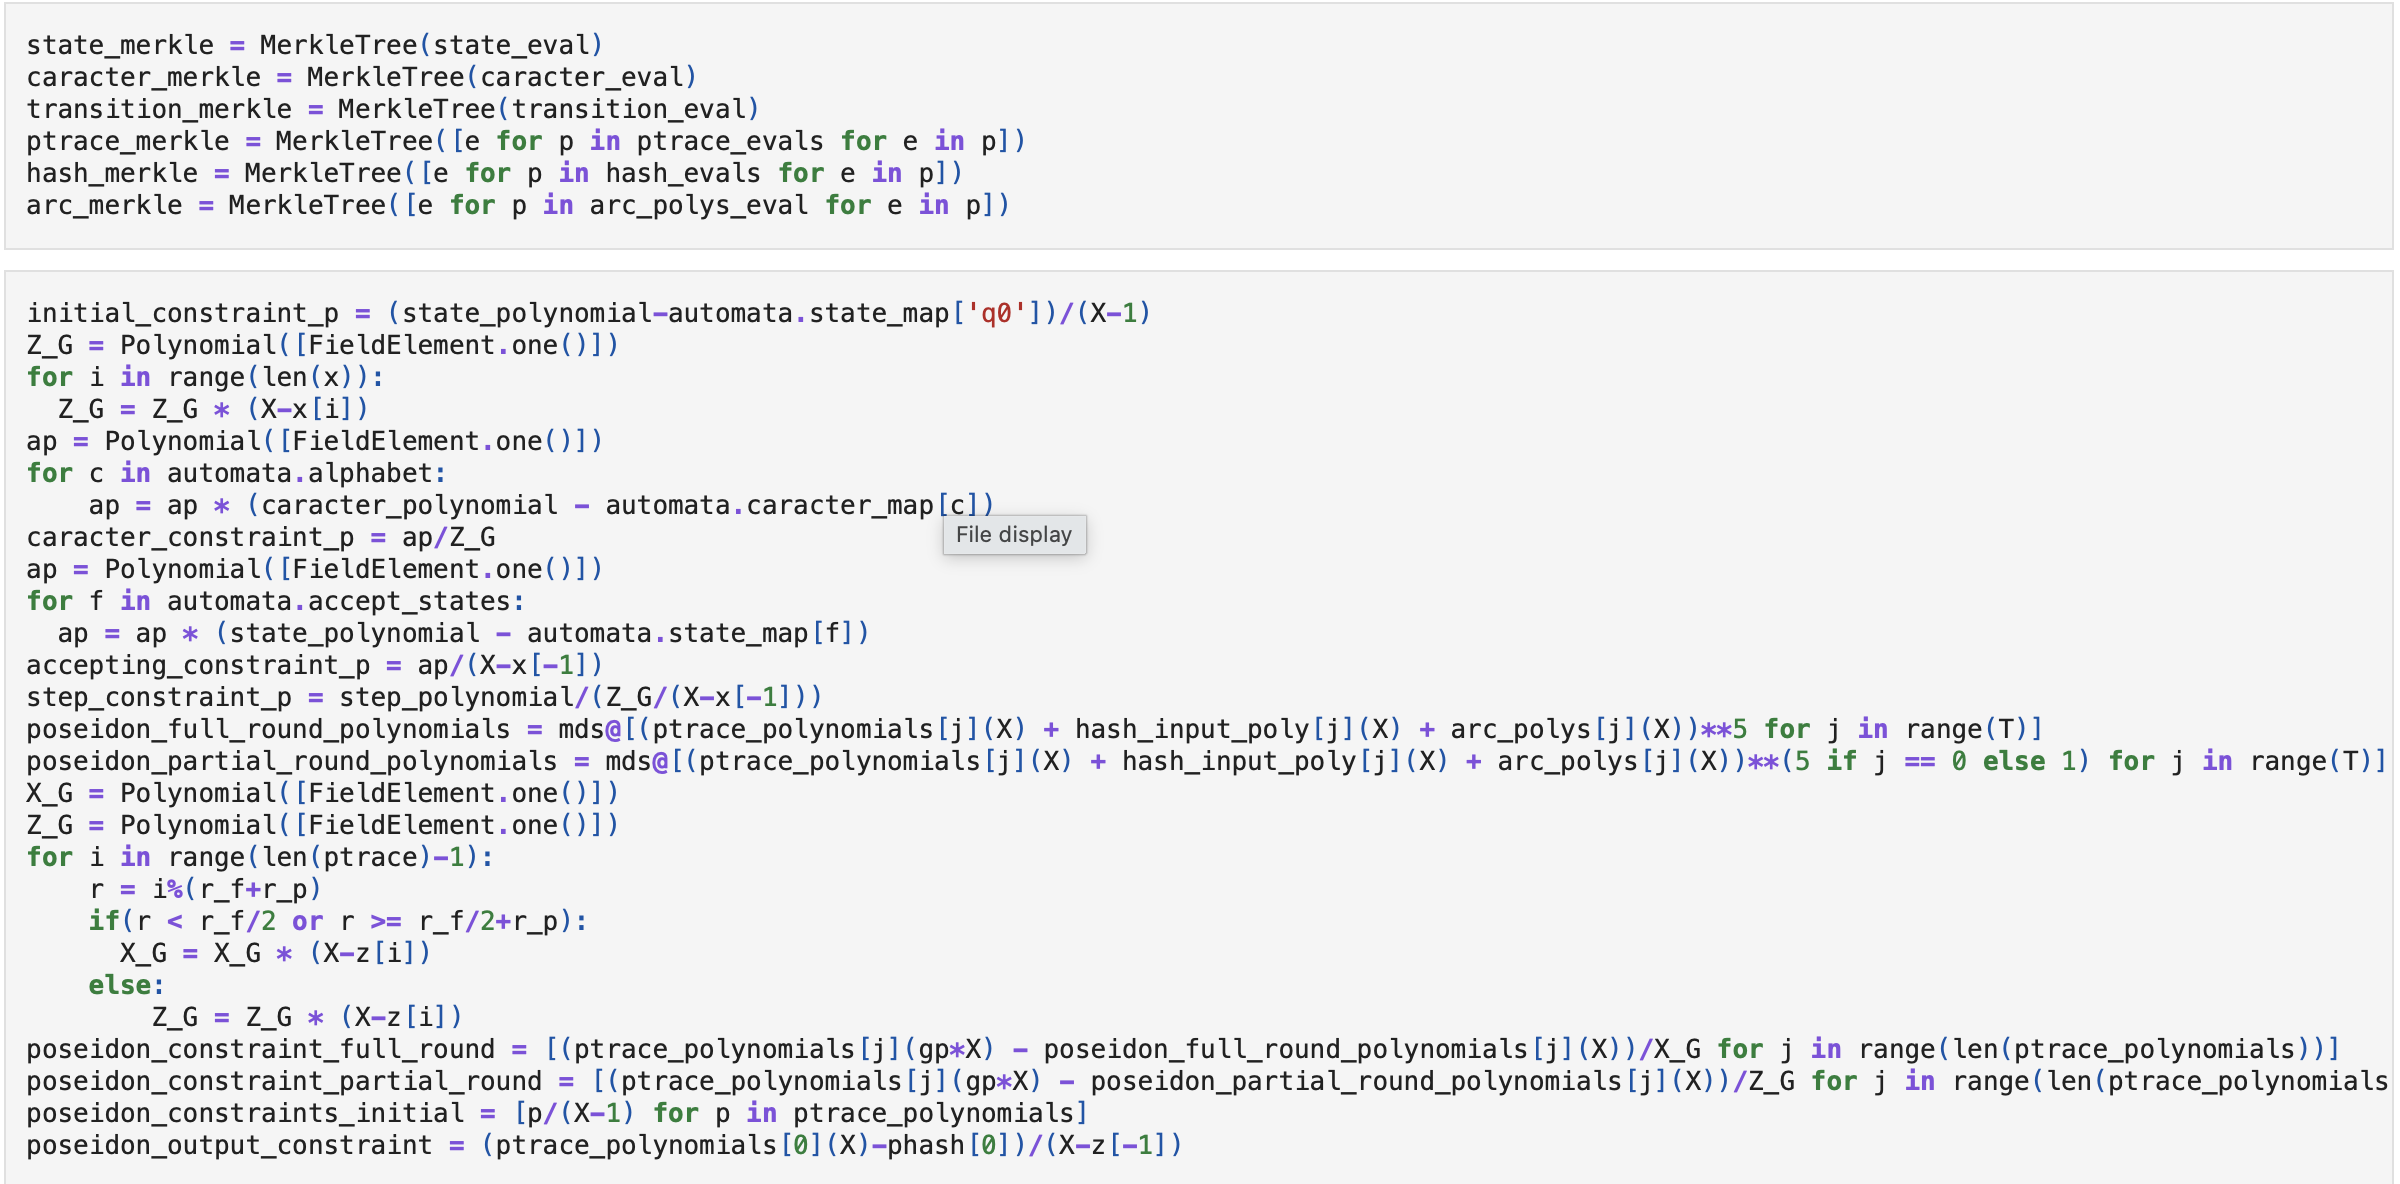
\includegraphics[width=0.8\textwidth]{10.png}
\end{figure}
\end{frame}
\begin{frame}
\frametitle{Annexe: Code}
\begin{figure}[h!]
  \centering
  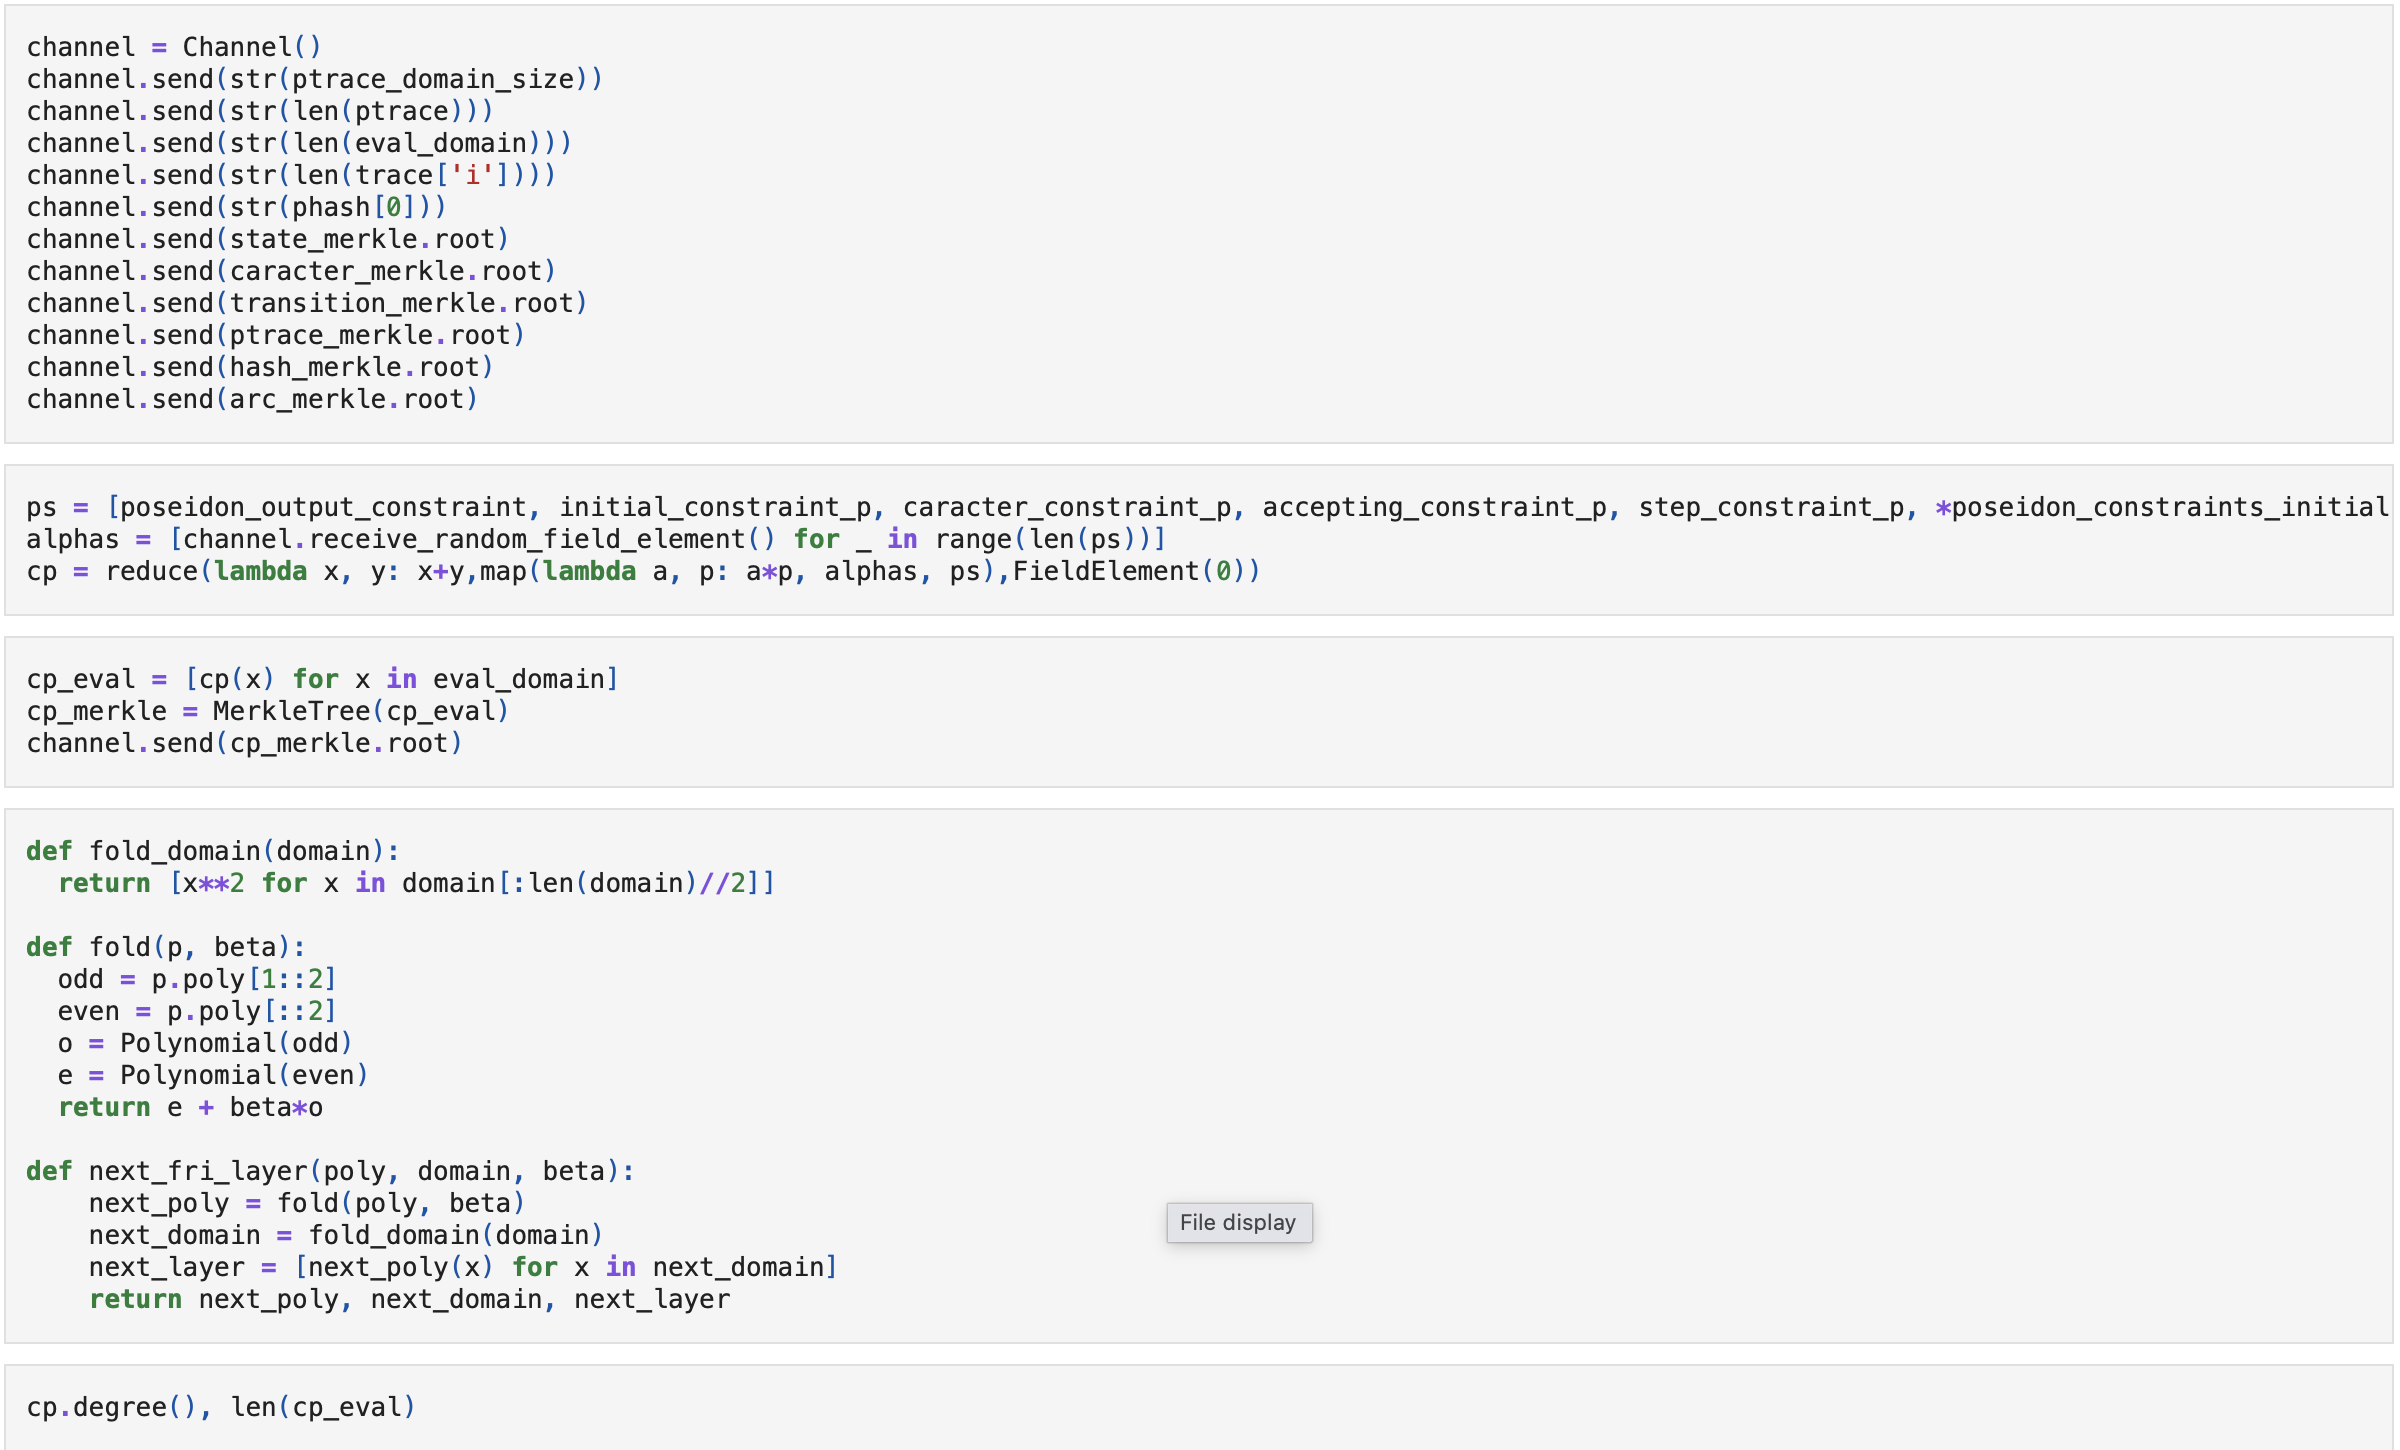
\includegraphics[width=0.8\textwidth]{11.png}
\end{figure}
\end{frame}
\begin{frame}
\frametitle{Annexe: Code}
\begin{figure}[h!]
  \centering
  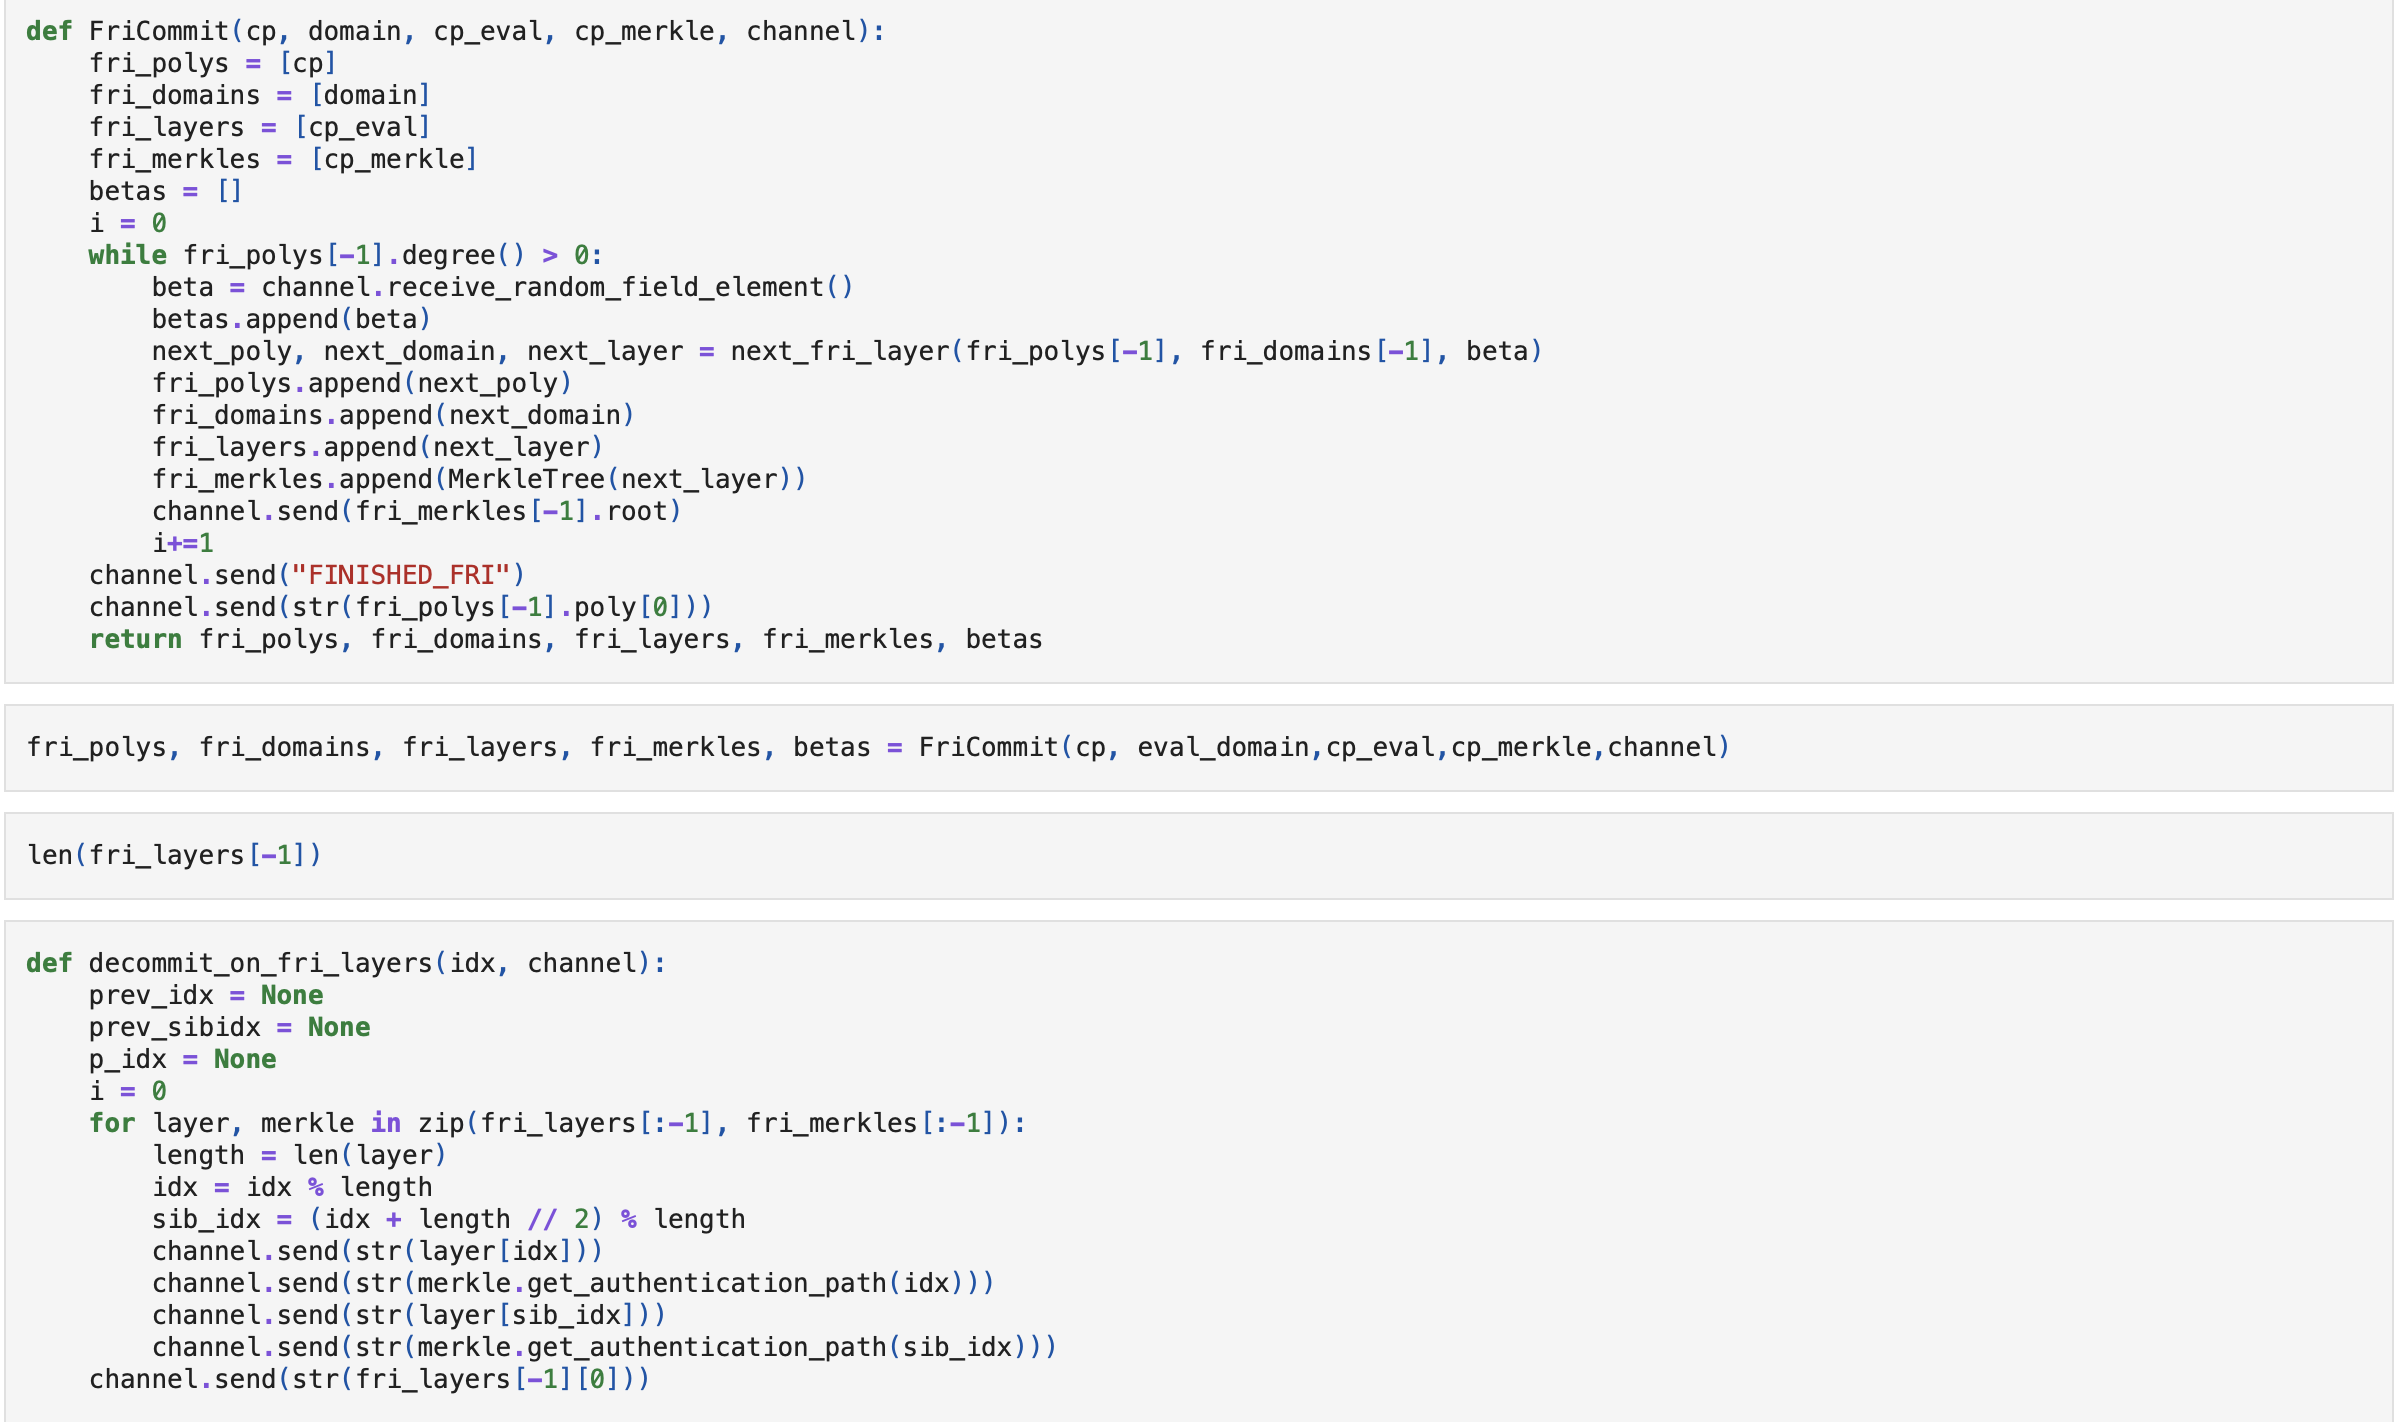
\includegraphics[width=0.8\textwidth]{12.png}
\end{figure}
\end{frame}
\begin{frame}
\frametitle{Annexe: Code}
\begin{figure}[h!]
  \centering
  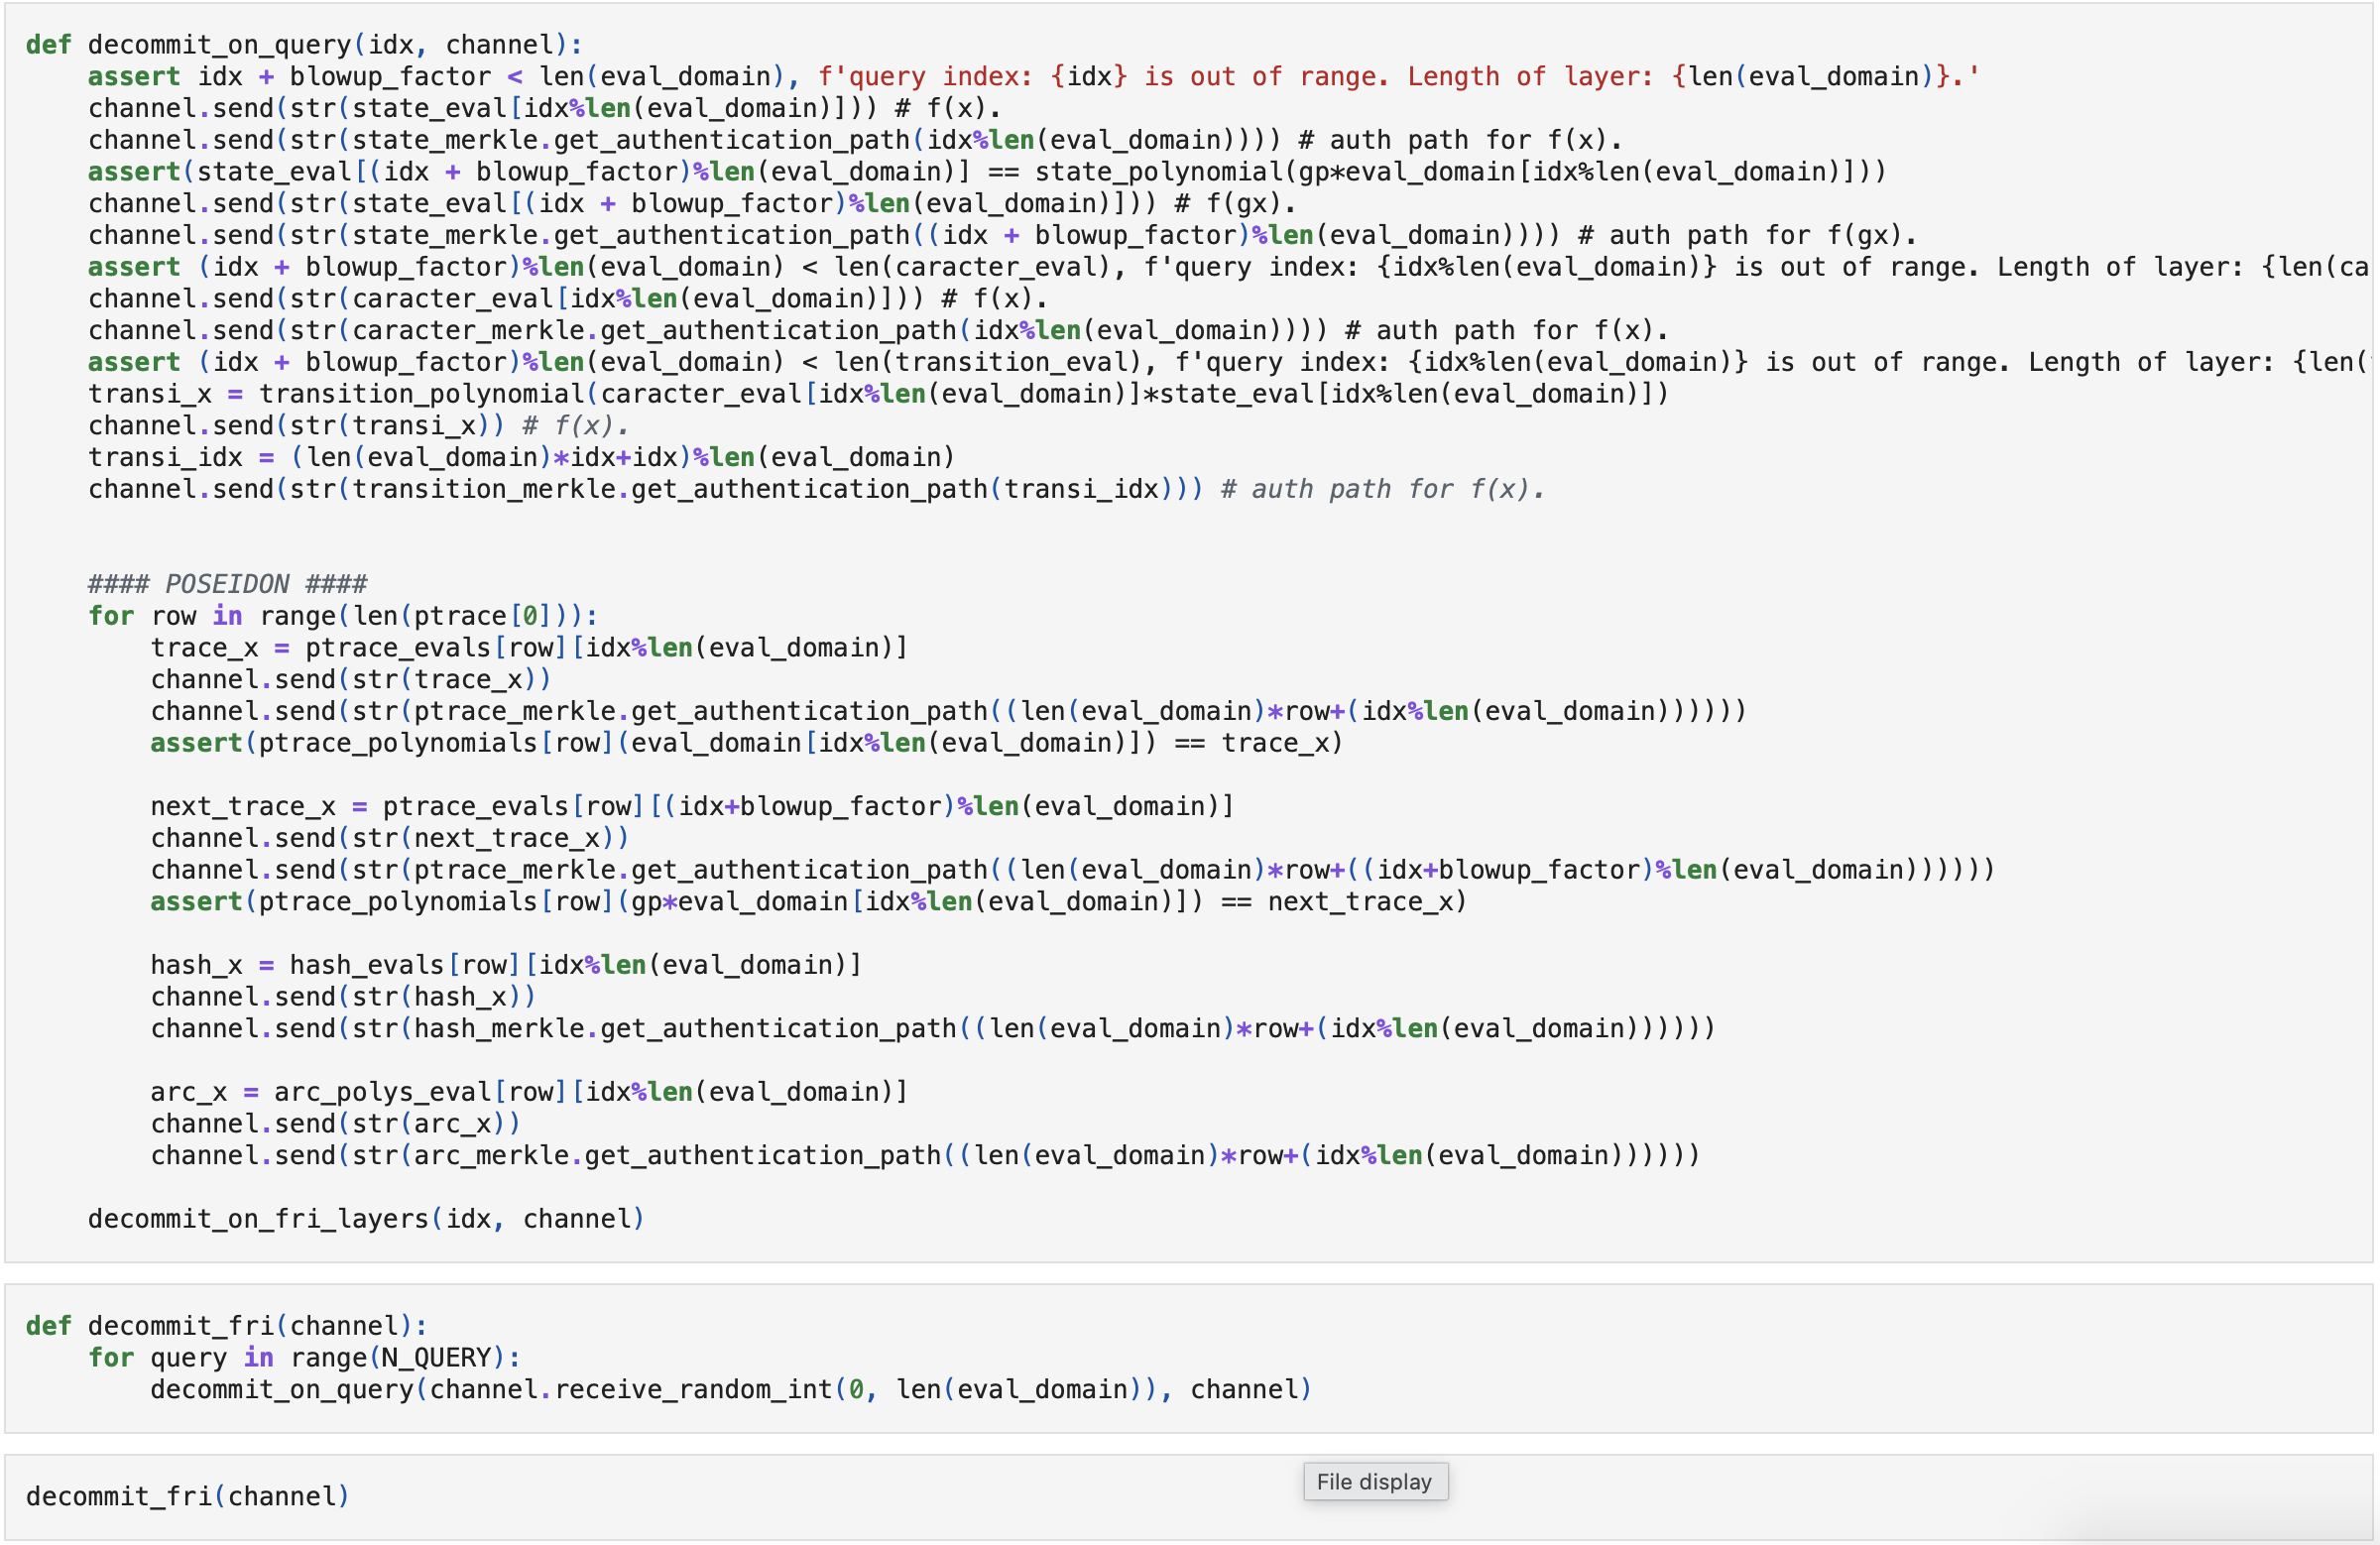
\includegraphics[width=0.8\textwidth]{13.png}
\end{figure}
\end{frame}
\begin{frame}
\frametitle{Annexe: Code}
\begin{figure}[h!]
  \centering
  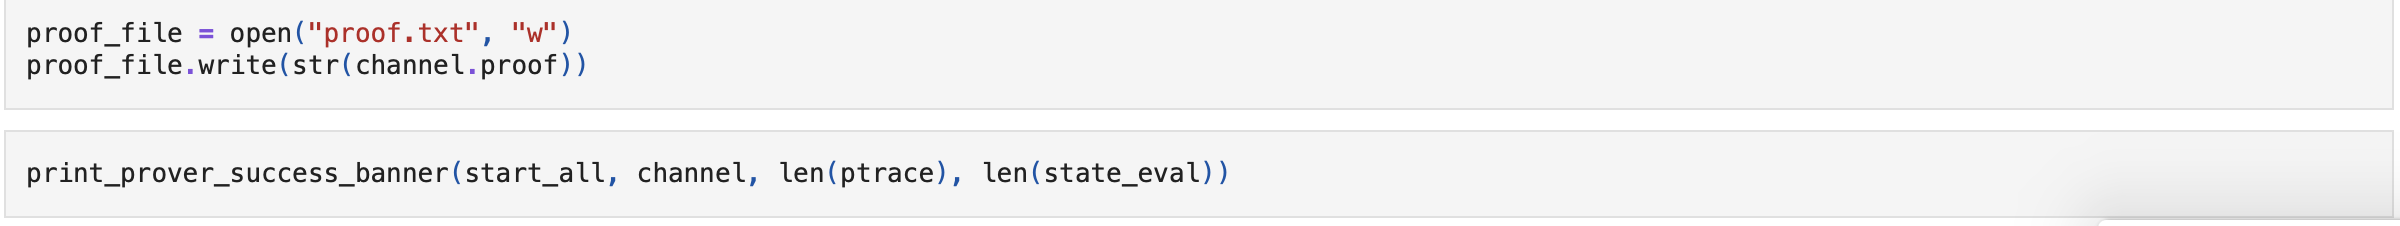
\includegraphics[width=0.8\textwidth]{14.png}
\end{figure}
\end{frame}
\begin{frame}
\frametitle{Annexe: Code}
\begin{figure}[h!]
  \centering
  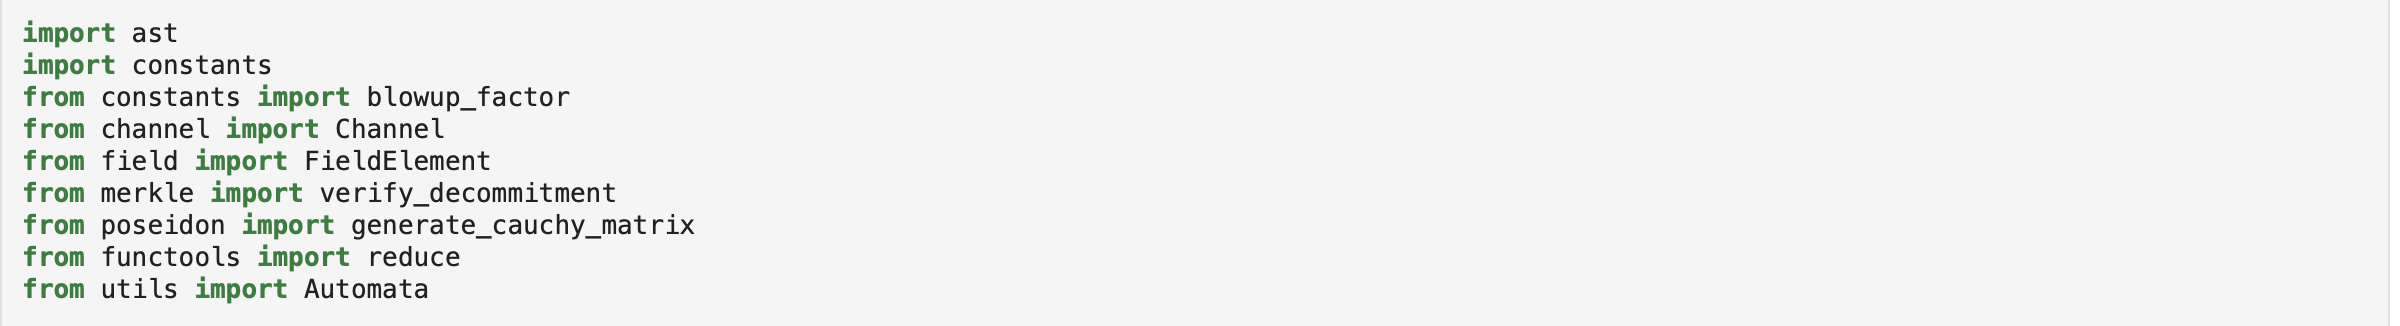
\includegraphics[width=0.8\textwidth]{15.png}
\end{figure}
\end{frame}
\begin{frame}
\frametitle{Annexe: Code}
\begin{figure}[h!]
  \centering
  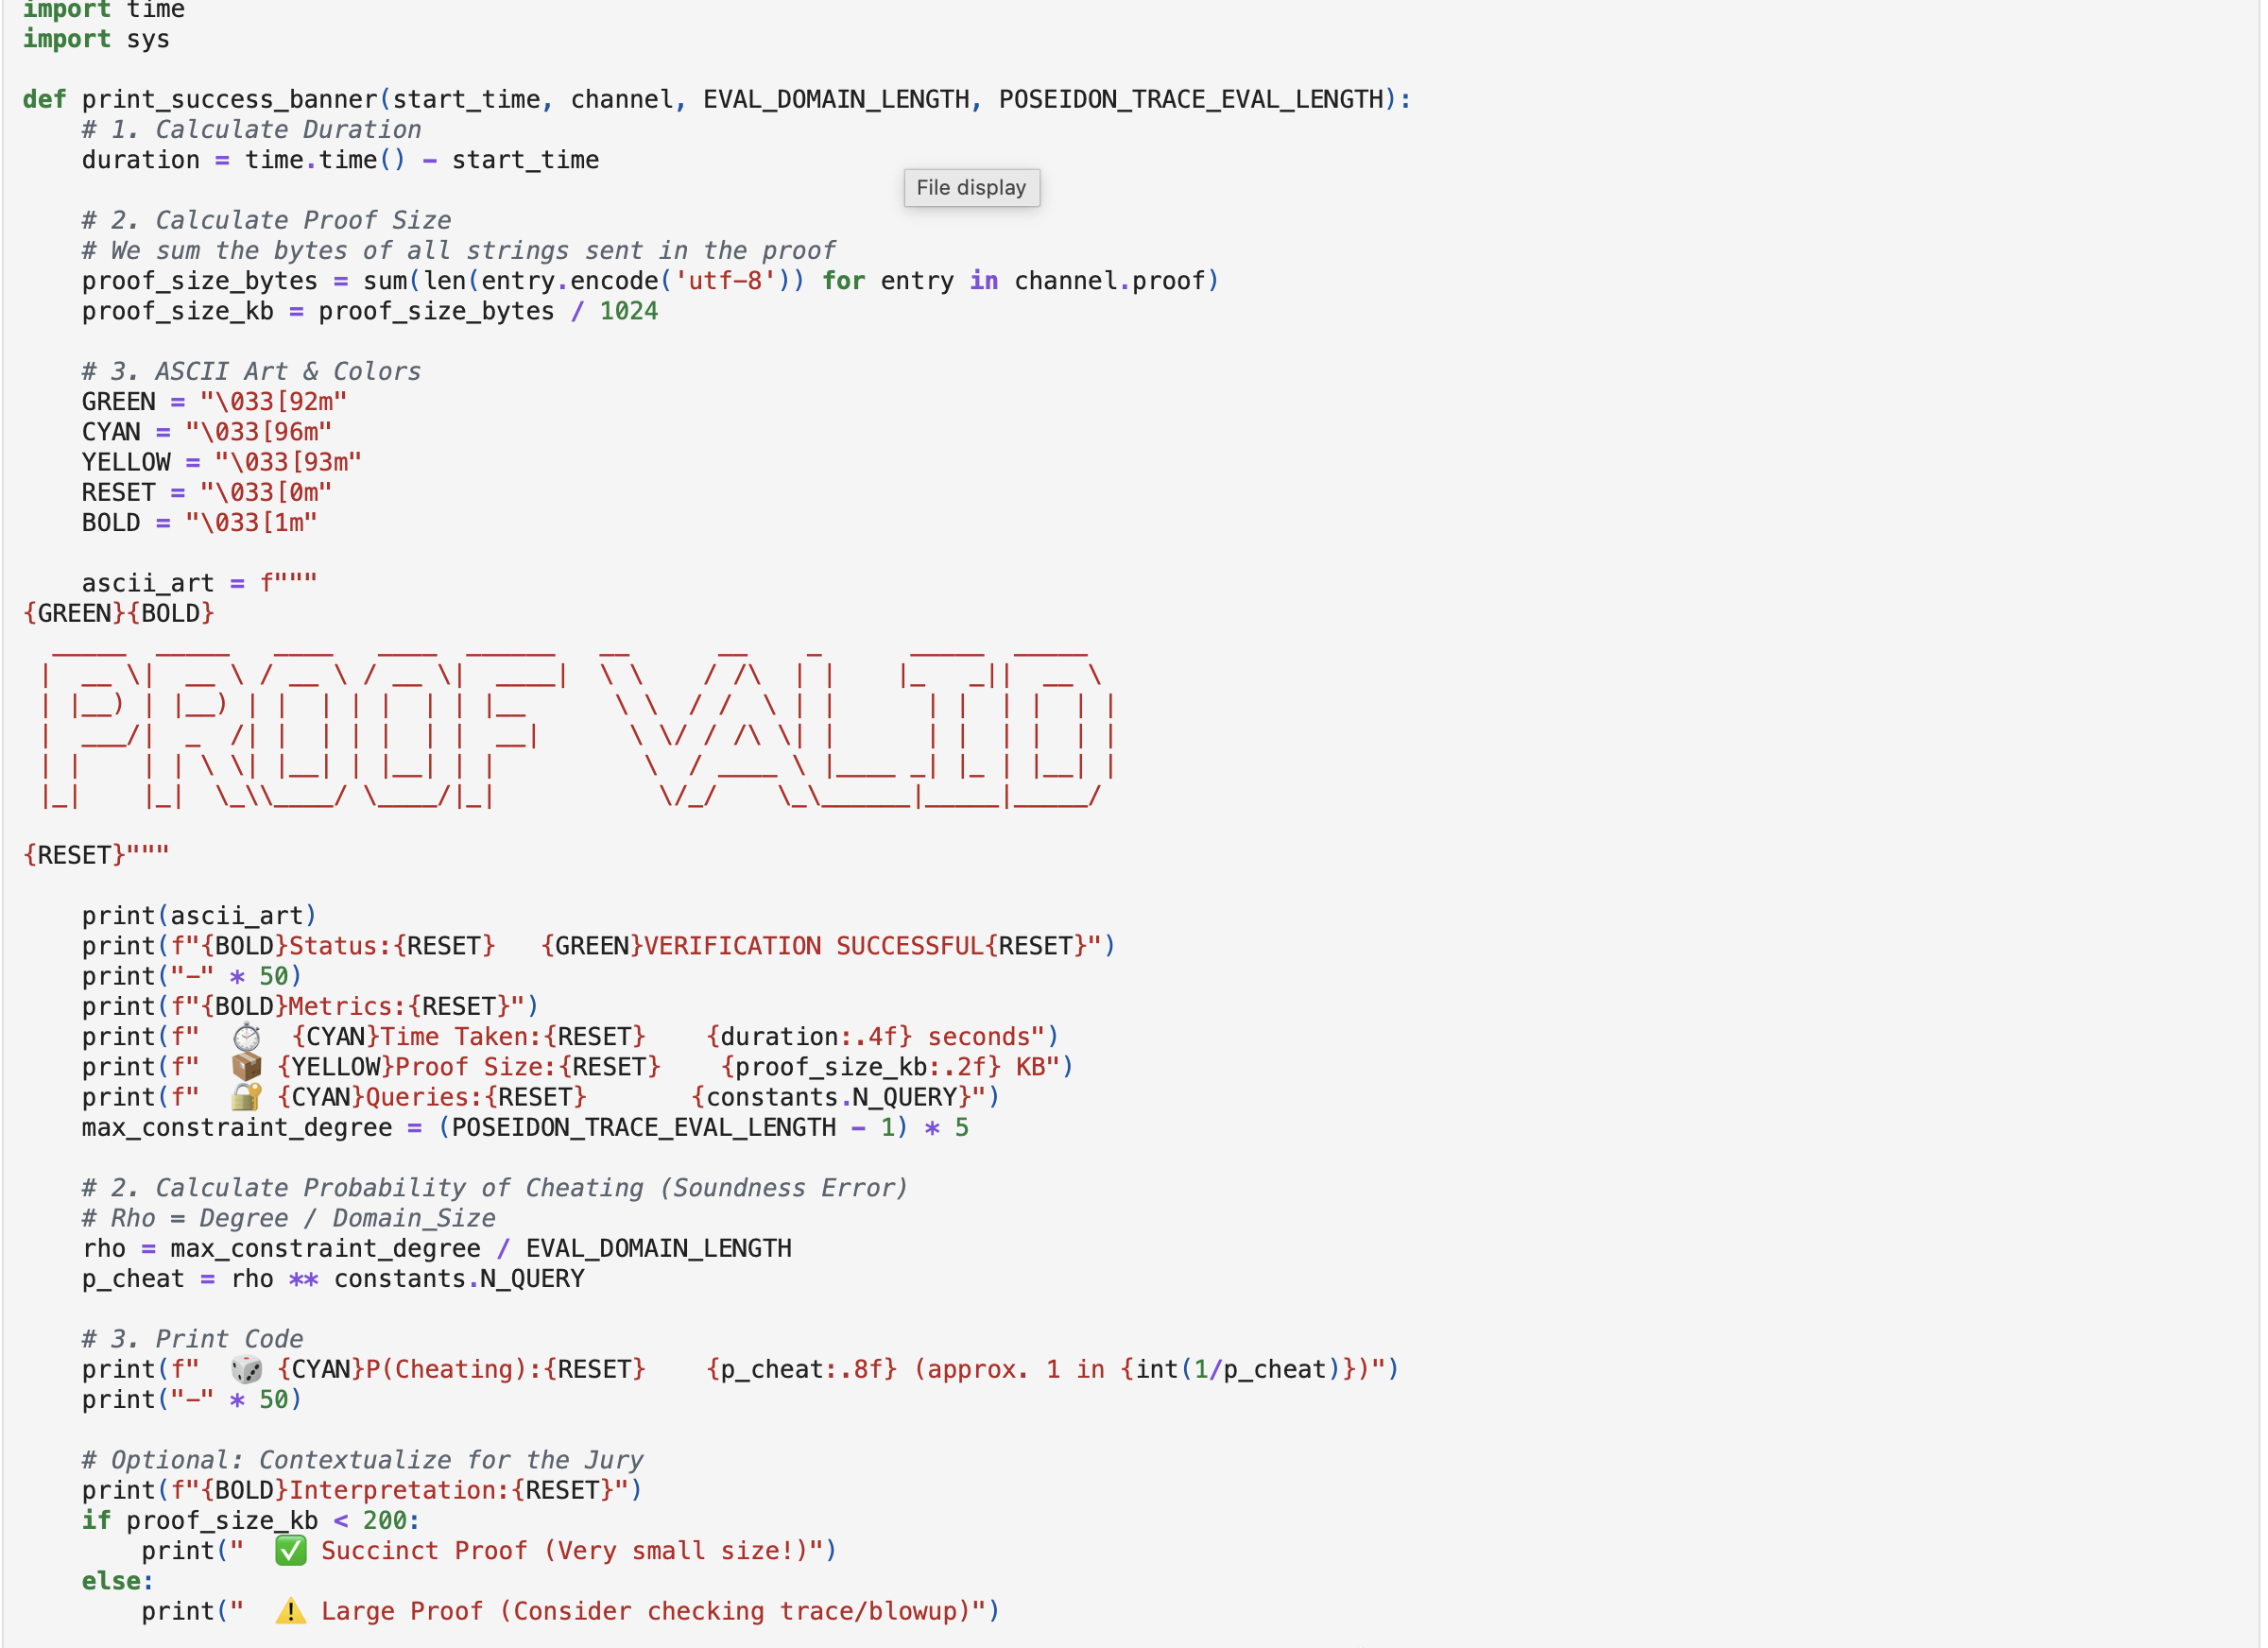
\includegraphics[width=0.8\textwidth]{16.png}
\end{figure}
\end{frame}
\begin{frame}
\frametitle{Annexe: Code}
\begin{figure}[h!]
  \centering
  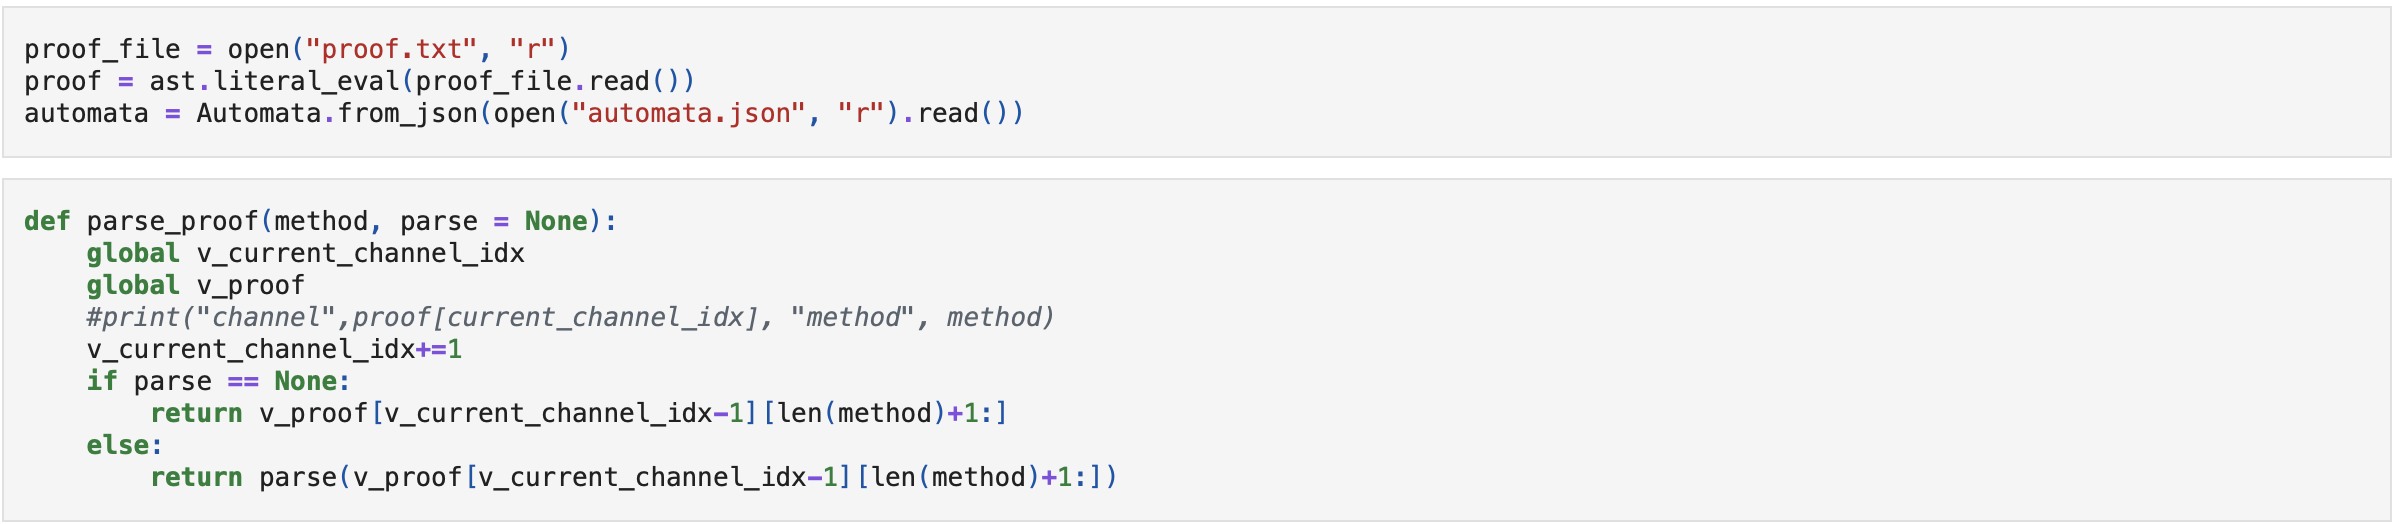
\includegraphics[width=0.8\textwidth]{17.png}
\end{figure}
\end{frame}
\begin{frame}
\frametitle{Annexe: Code}
\begin{figure}[h!]
  \centering
  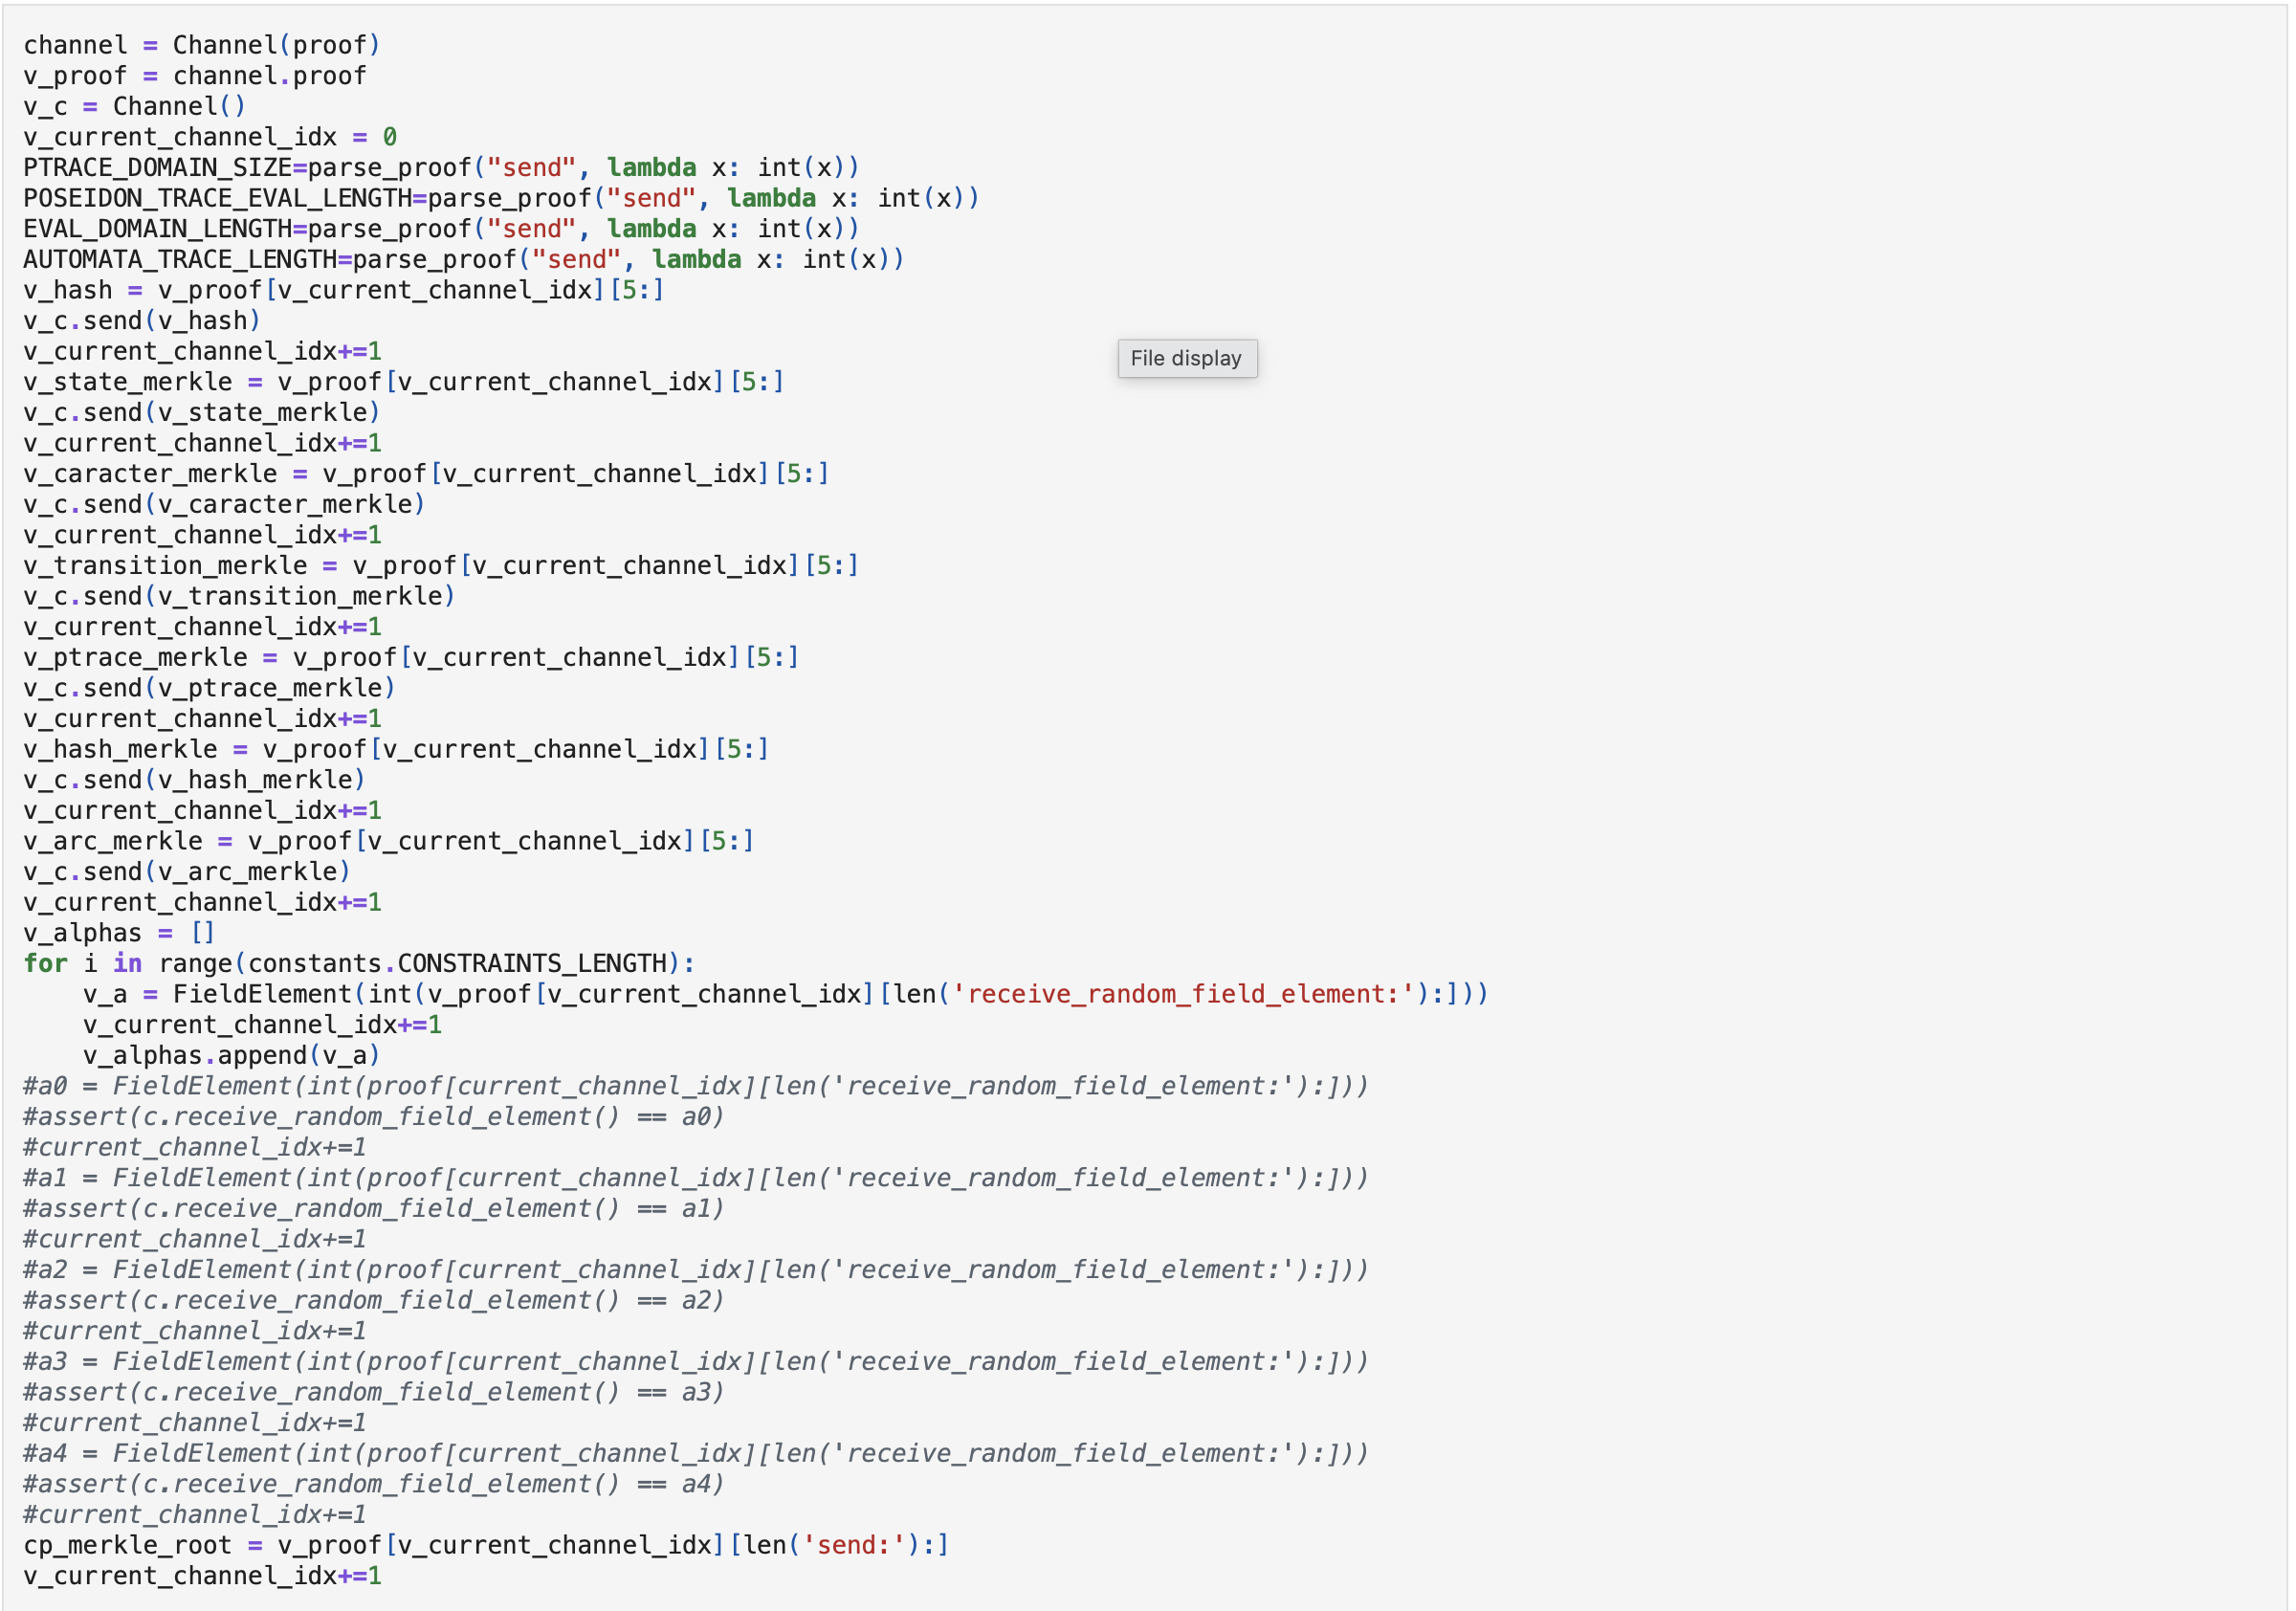
\includegraphics[width=0.8\textwidth]{18.png}
\end{figure}
\end{frame}
\begin{frame}
\frametitle{Annexe: Code}
\begin{figure}[h!]
  \centering
  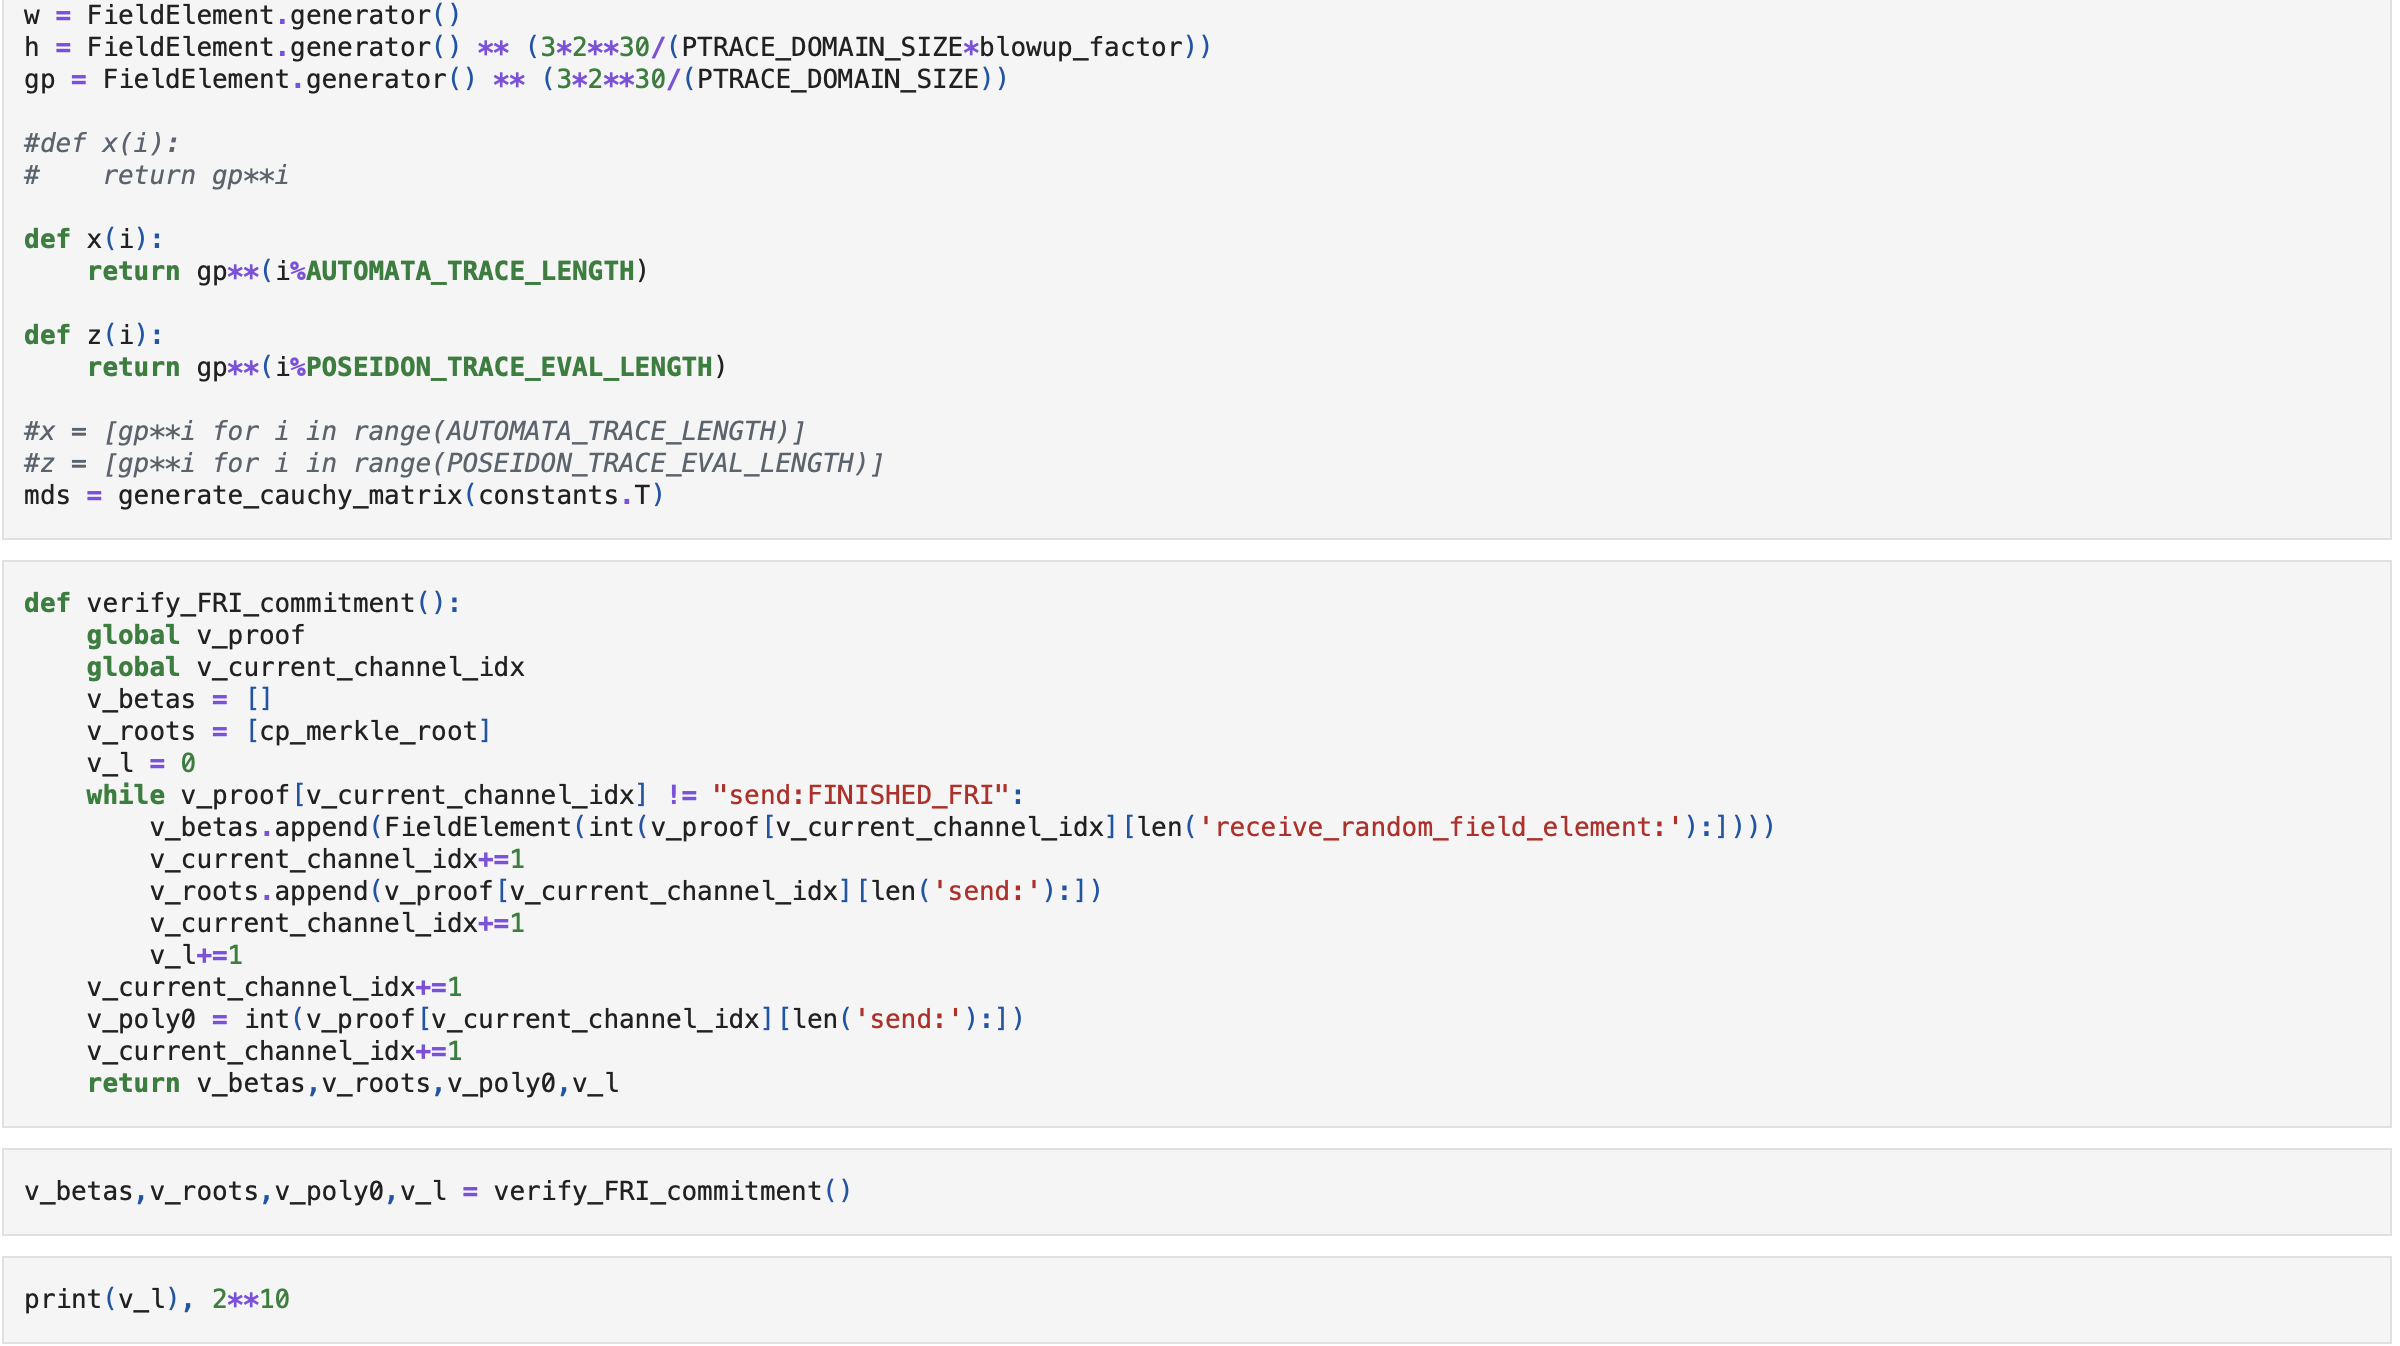
\includegraphics[width=0.8\textwidth]{19.png}
\end{figure}
\end{frame}
\begin{frame}
\frametitle{Annexe: Code}
\begin{figure}[h!]
  \centering
  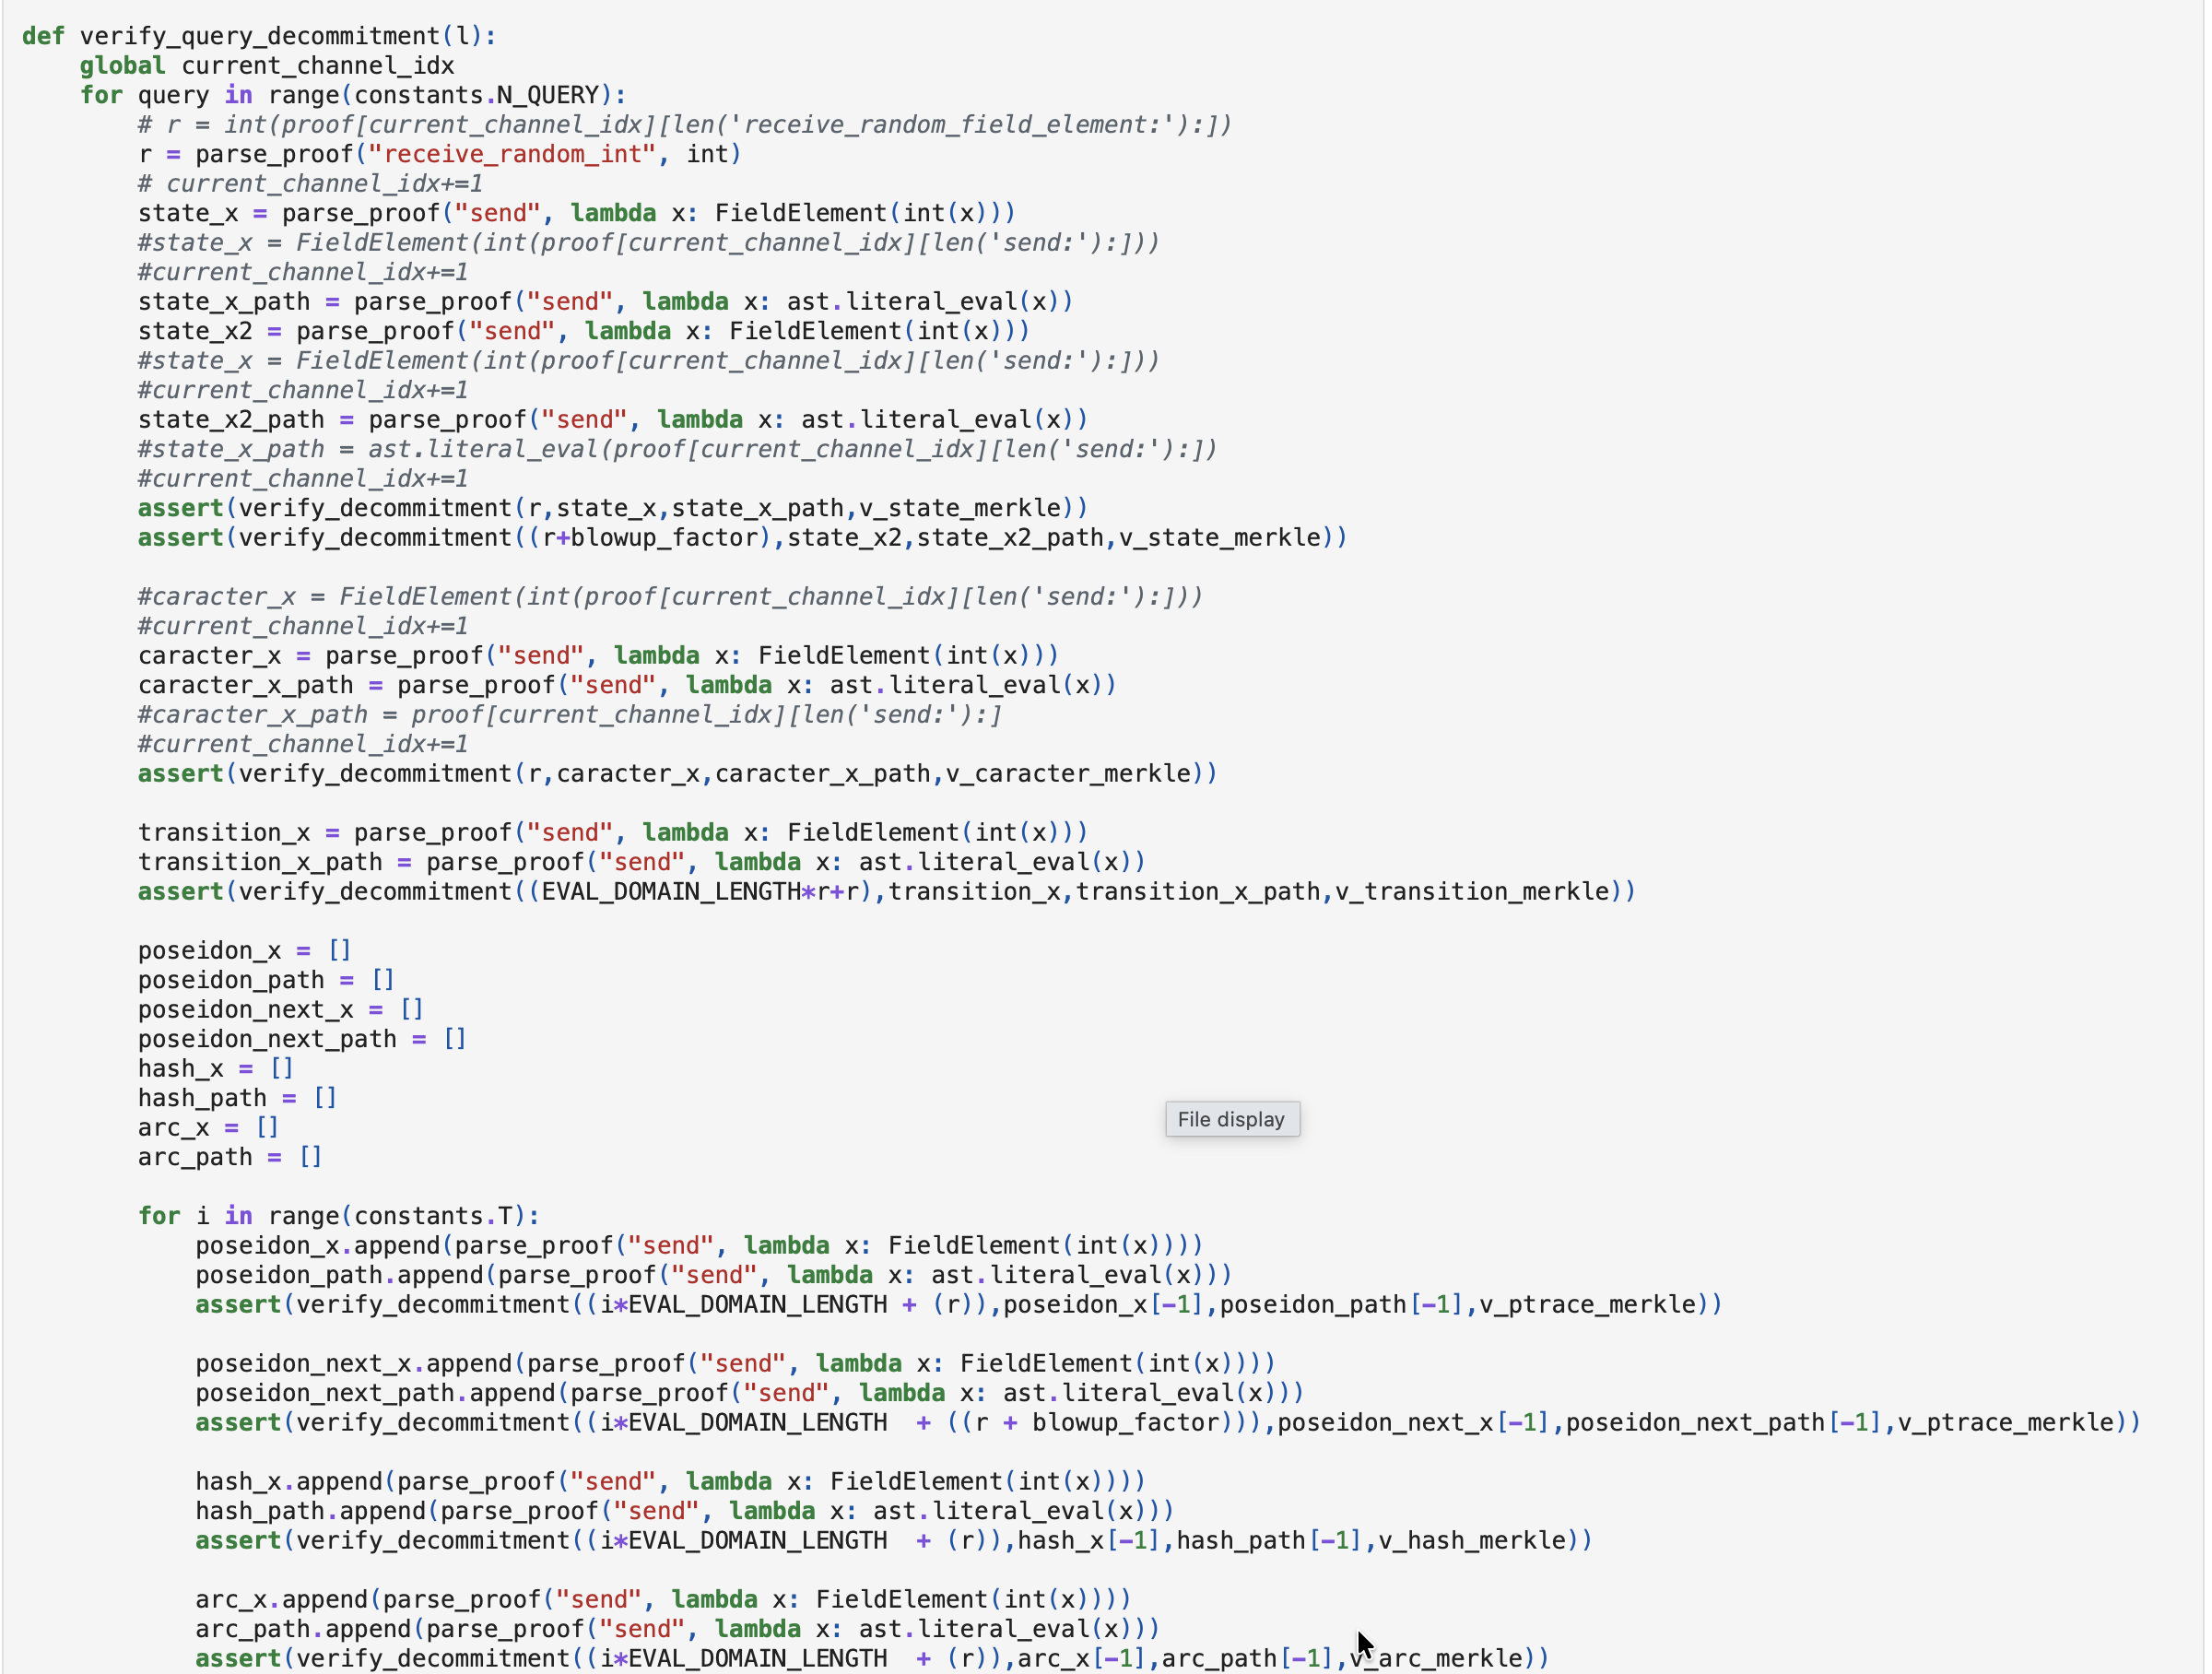
\includegraphics[width=0.8\textwidth]{20.png}
\end{figure}
\end{frame}
\begin{frame}
\frametitle{Annexe: Code}
\begin{figure}[h!]
  \centering
  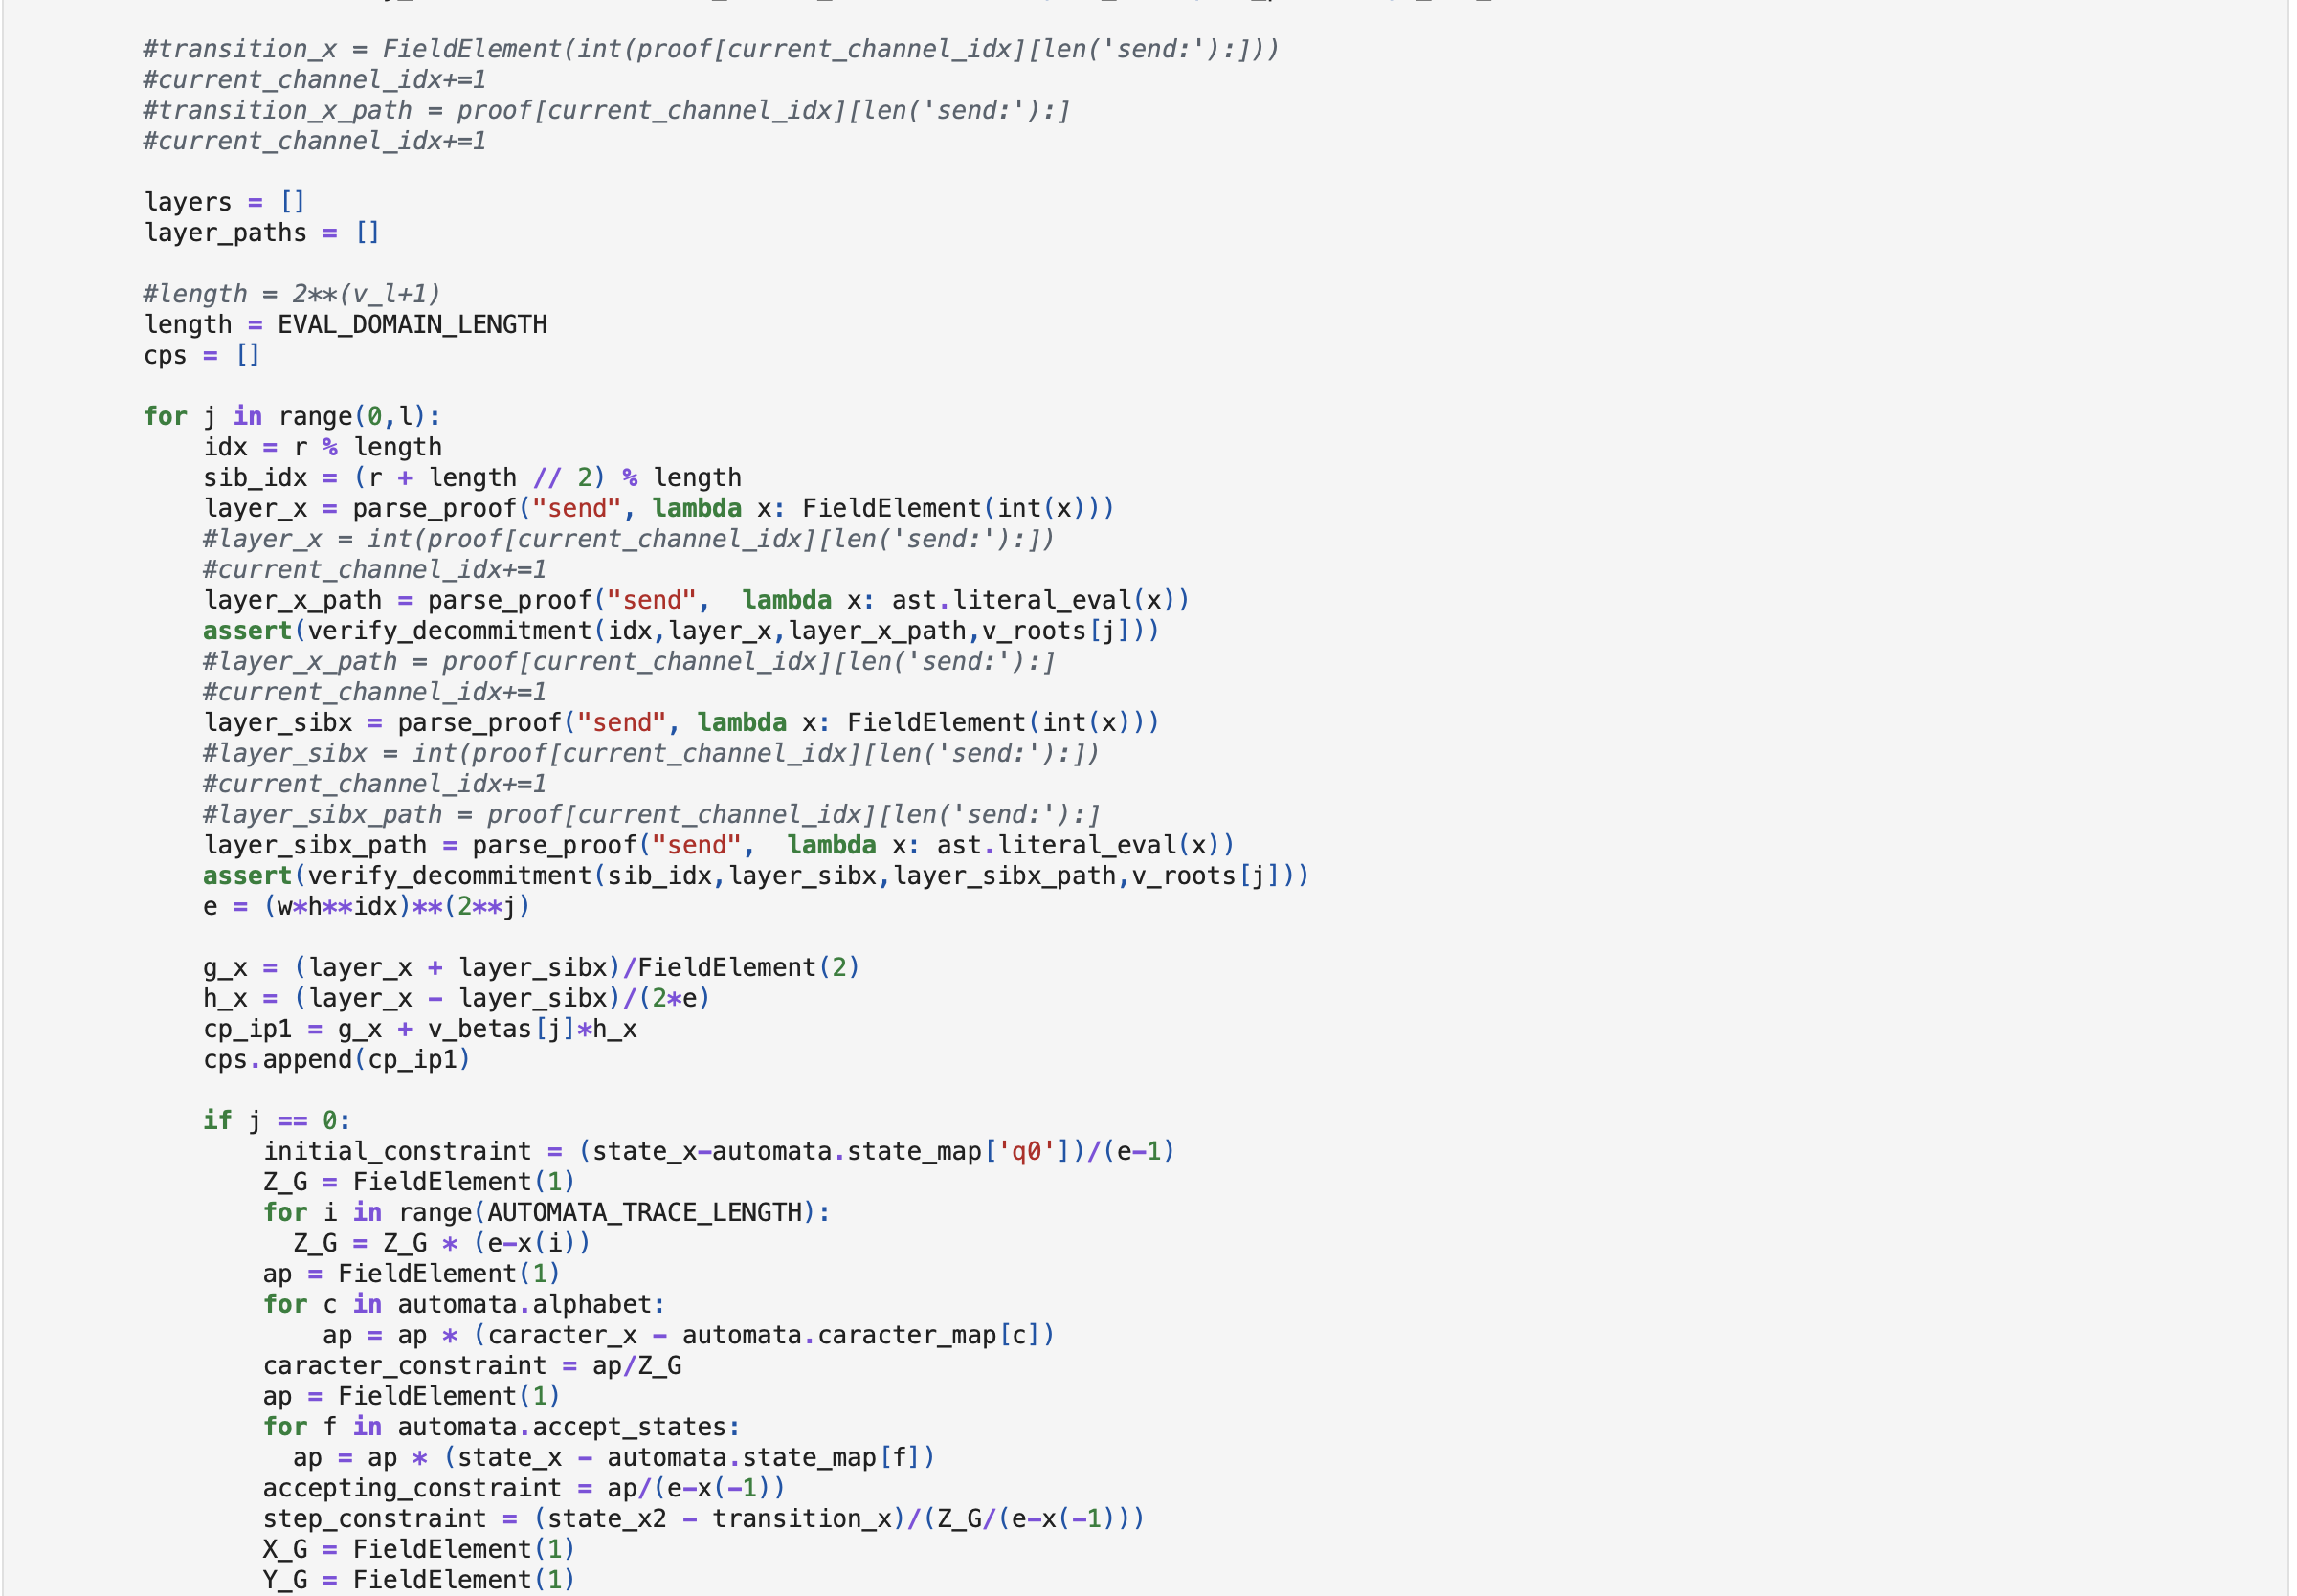
\includegraphics[width=0.8\textwidth]{21.png}
\end{figure}
\end{frame}
\begin{frame}
\frametitle{Annexe: Code}
\begin{figure}[h!]
  \centering
  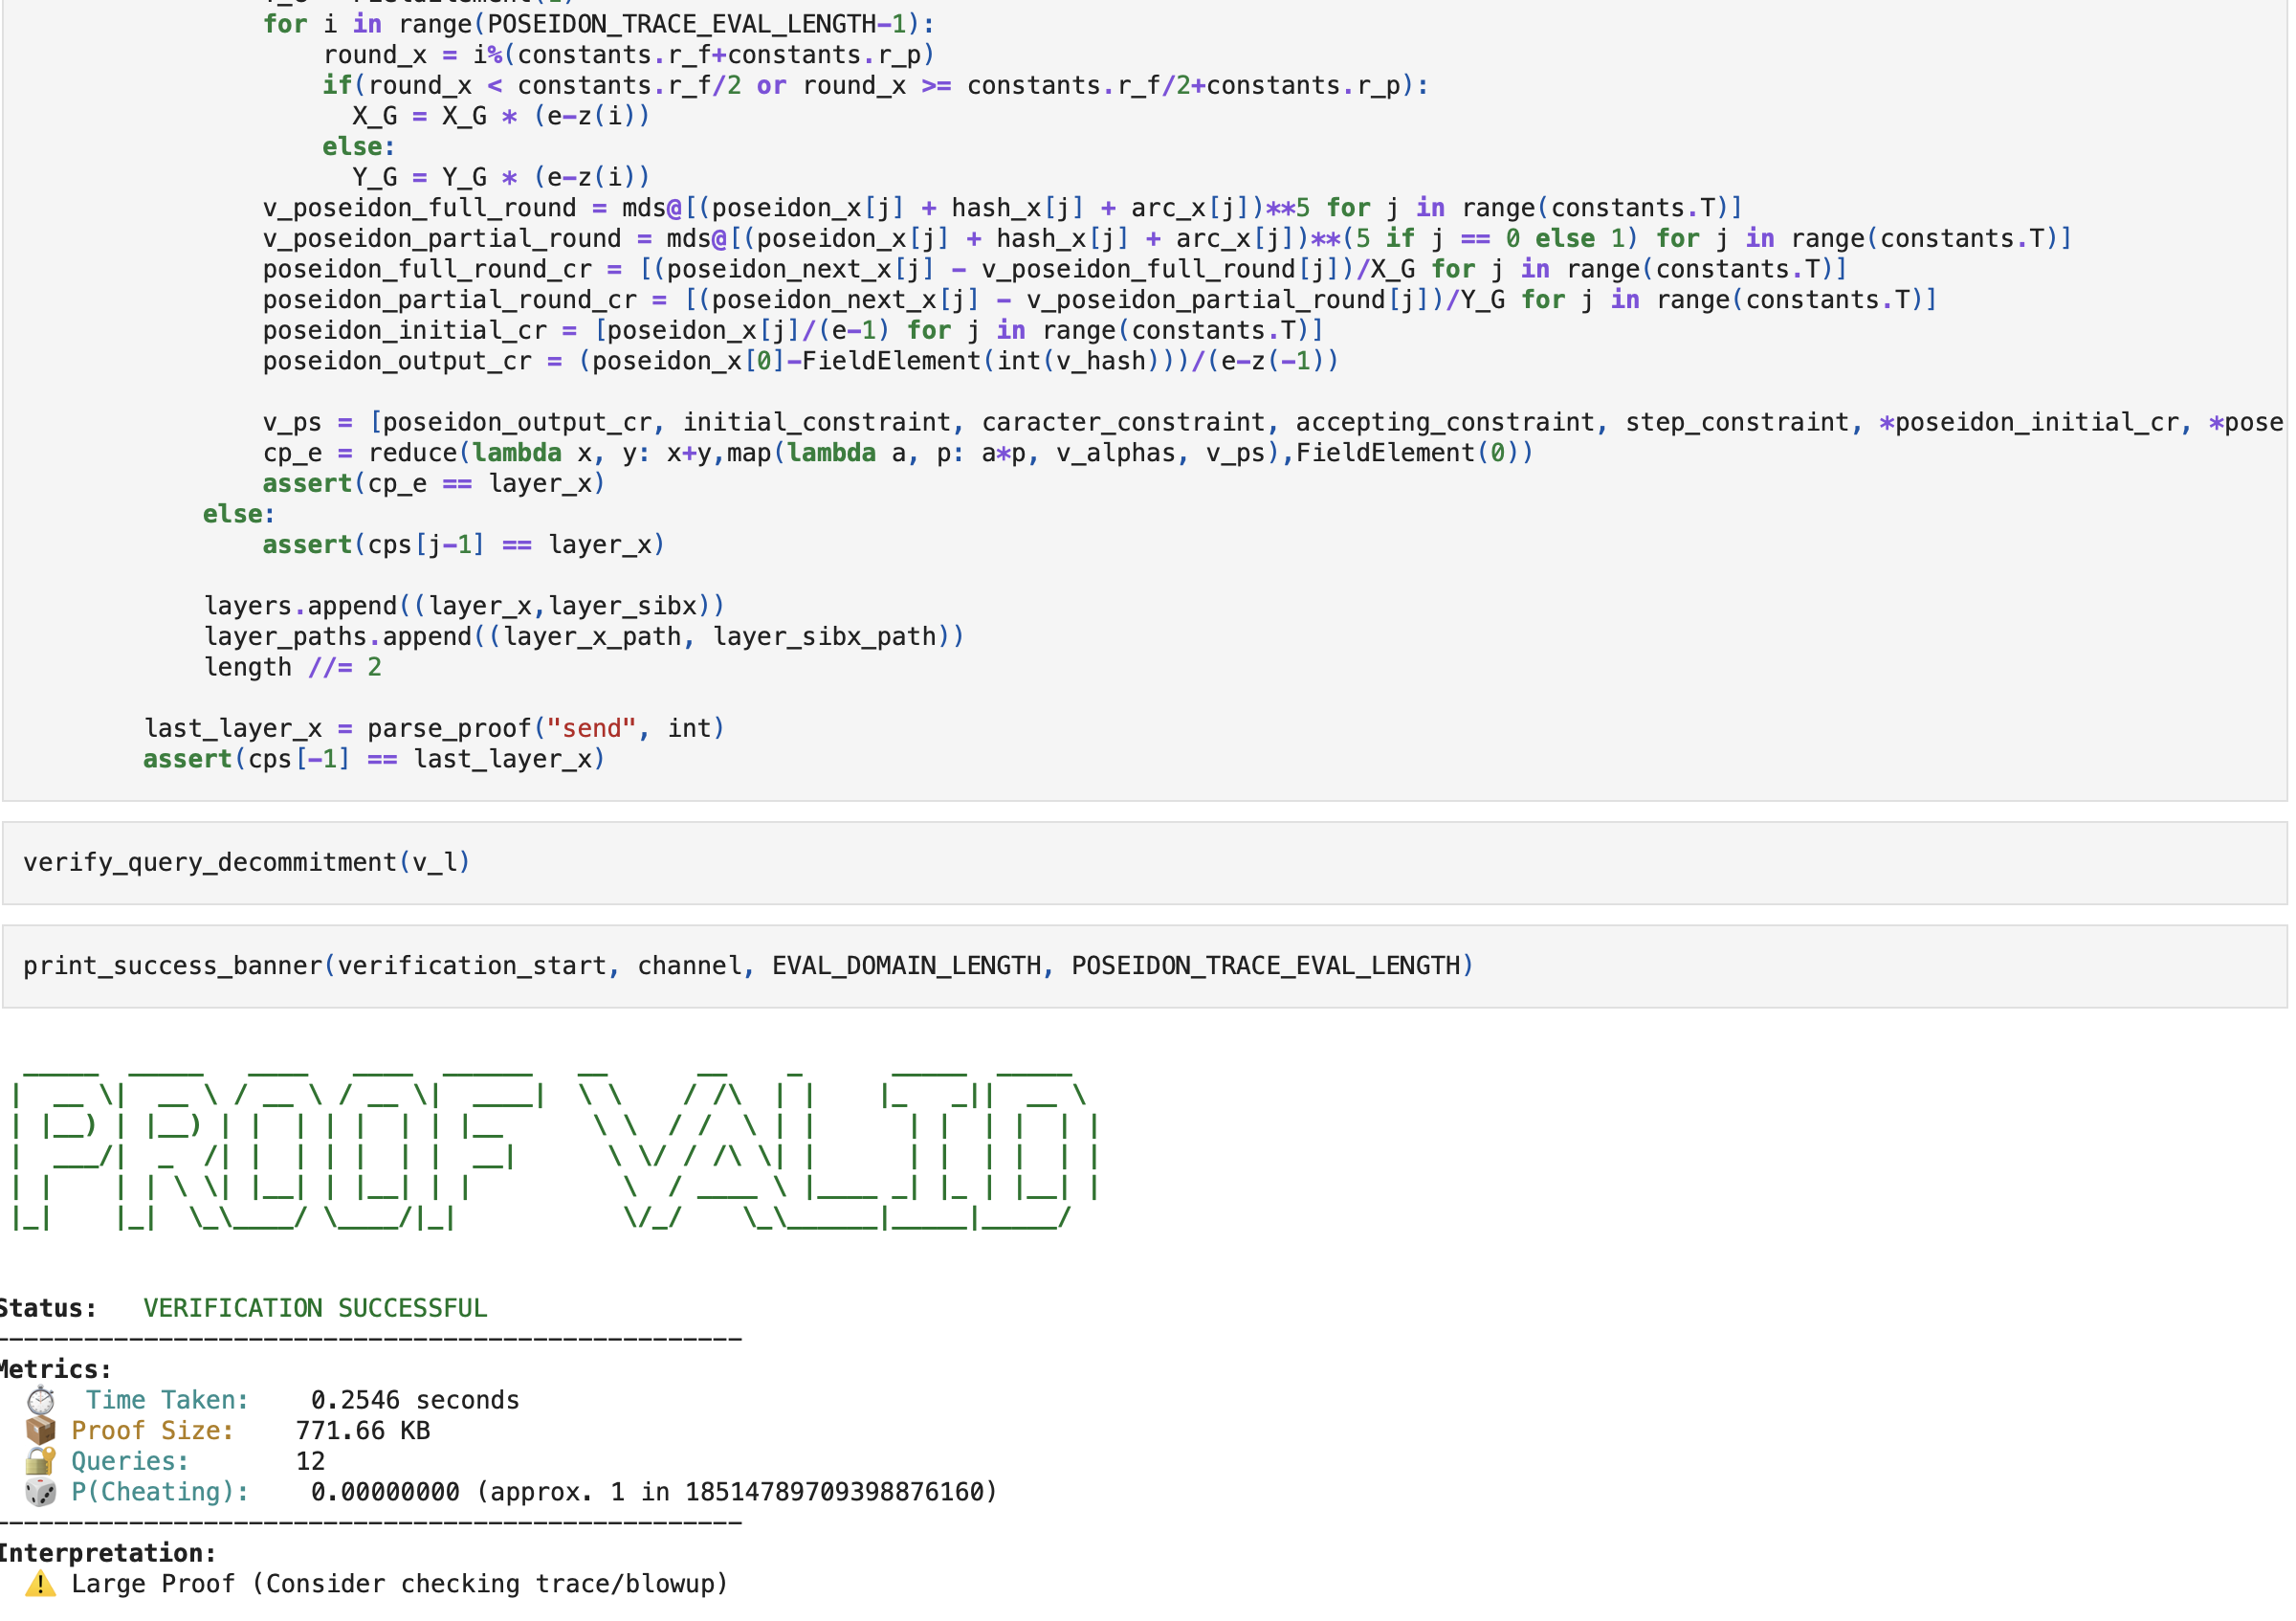
\includegraphics[width=0.8\textwidth]{22.png}
\end{figure}
\end{frame}
\end{document}
